%\documentclass[11pt, color=none]{elegantbook}
%\documentclass{[11pt]{book}}
\documentclass{kumikoNotes}


\setcounter{tocdepth}{2}
\title{\Huge{Smooth Manifolds}}
%\subtitle{}

\author{Kumiko}
\date{2023 spring}
%\version{4.3}
%\bioinfo{Bio}{Information}

%\logo{logo-blue.png}

% modify the color in the middle of titlepage

\begin{document}
% ============= summation, product =============



\newcommand{\Sum}[2]{\sum_{#1}^{#2}}
\newcommand{\SumInf}[1]{\sum_{#1}^{\infty}}
\newcommand{\Prod}[2]{\prod_{#1}^{#2}}

\newcommand{\suminfty}[2]{\sum_{#1 = #2}^{\infty}} %inf sum
\newcommand{\sumfin}[3]{\sum_{#1 = #2}^{#3}} %\sumfin{i}{0}{N}
\newcommand{\integrate}[4]{\int_{#1}^{#2} #3 ~d#4}

\newcommand{\oProd}[2]{\bigotimes_{#1}^{#2}} % product sigma-algebra

\newcommand{\cdTimes}{\times \cdots \times} % x ... x
\newcommand{\cdOtimes}{\otimes \cdots \otimes}
\newcommand{\cdWedge}{\wedge \cdots \otimes}

% ============= set & topological operations =============
\newcommand{\union}[2]{\cup_{#1}^{#2}}
\newcommand{\intersect}[2]{\cap_{#1}^{#2}}
\newcommand{\bigunion}[2]{\bigcup_{#1}^{#2}}
\newcommand{\bigintersect}[2]{\bigcap_{#1}^{#2}}
\newcommand{\bCup}[2]{\bigcup_{#1}^{#2}}
\newcommand{\bCap}[2]{\bigcap_{#1}^{#2}}

\newcommand{\cl}[1]{\overline{#1}} % closure of a set

% ============ Greek =================
\renewcommand{\a}{\alpha}
\renewcommand{\b}{\beta}
\renewcommand{\d}{\delta}
\newcommand{\eps}{\varepsilon}
\newcommand{\lam}{\lambda}
\newcommand{\Lam}{\Lambda}
\newcommand{\s}{\sigma}
\newcommand{\omg}{\omega}
\newcommand{\Omg}{\Omega}
\newcommand{\Ga}{\Gamma}
\newcommand{\ga}{\gamma}
%\newcommand{\th}{\theta}
\newcommand{\vphi}{\varphi}
\newcommand{\phe}{\varphi}
\newcommand{\cta}{\theta}


% ============ mathbb ================
\newcommand{\E}{\mathbb{E}}
\newcommand{\F}{\mathbb{F}}
\renewcommand{\P}{\mathbb{P}}
\newcommand{\Q}{\mathbb{Q}}
\newcommand{\R}{\mathbb{R}}
\newcommand{\C}{\mathbb{C}}
\newcommand{\N}{\mathbb{N}}
\newcommand{\Z}{\mathbb{Z}}
\renewcommand{\S}{\mathbb{S}}

\newcommand{\T}{\mathbb{T}}
\newcommand{\bbT}{\mathbb{T}}
\newcommand{\D}{\mathbb{D}}
\newcommand{\B}{\mathbb{B}}
\renewcommand{\H}{\mathbb{H}}

% ============ calligraphy =============
\newcommand{\Cal}[1]{\mathcal{#1}}
\newcommand{\calA}{\mathcal{A}}
\newcommand{\calB}{\mathcal{B}}
\newcommand{\calC}{\mathcal{C}}
\newcommand{\calD}{\mathcal{D}}
\newcommand{\calE}{\mathcal{E}}
\newcommand{\calF}{\mathcal{F}}
\newcommand{\calG}{\mathcal{G}}
\newcommand{\calH}{\mathcal{H}}
\newcommand{\calI}{\mathcal{I}}
\newcommand{\calJ}{\mathcal{J}}

\newcommand{\calL}{\mathcal{L}}
\newcommand{\calM}{\mathcal{M}}
\newcommand{\calN}{\mathcal{N}}
\newcommand{\calO}{\mathcal{O}}
\newcommand{\calP}{\mathcal{P}}
\newcommand{\calQ}{\mathcal{Q}}
\newcommand{\calR}{\mathcal{R}}
\newcommand{\calS}{\mathcal{S}}
\newcommand{\calT}{\mathcal{T}} % topology

\newcommand{\calU}{\mathcal{U}}
\newcommand{\calV}{\mathcal{V}}
\newcommand{\calX}{\mathcal{X}}
\newcommand{\calY}{\mathcal{Y}}

\newcommand{\frakX}{\mathfrak{X}}

% ============ category theory: sans-serif ================
\newcommand{\sfC}{\mathsf{C}}
\newcommand{\sfD}{\mathsf{D}}
\newcommand{\sfSet}{\mathsf{Set}}
\newcommand{\sfTop}{\mathsf{Top}}
\newcommand{\sfMan}{\mathsf{Man}}
\newcommand{\sfDiff}{\mathsf{Diff}}
\newcommand{\sfVec}{\mathsf{Vec}}
\newcommand{\sfGrp}{\mathsf{Grp}}
\newcommand{\sfAb}{\mathsf{Ab}}
\newcommand{\sfRng}{\mathsf{Rng}}
\newcommand{\sfCRng}{\mathsf{CRng}}

\newcommand{\Ob}{\mathrm{Ob}}
\newcommand{\Hom}{\mathrm{Hom}}



% ============= braces ==============
\newcommand{\curlBrace}[1]{\left\{#1\right\}}
\newcommand{\Brace}[1]{\left(#1\right)}
\newcommand{\net}[1]{\left\langle #1 \right\rangle} % inner product
\newcommand{\Abs}[1]{\left|#1\right|} % absolute value
\newcommand{\Lnorm}[2]{\norm{#1}_{L^{#2}}} % L^p norm
\renewcommand{\hat}{\widehat}
\newcommand{\br}[1]{\left(#1\right)}
\newcommand{\cBr}[1]{\left\{#1\right\}}

% ============= colors ==============
\newcommand{\red}[1]{\textcolor{red}{#1}}
\newcommand{\cyan}[1]{\textcolor{cyan}{#1}}
\newcommand{\NvBlue}[1]{\textcolor{NavyBlue}{#1}}
\newcommand{\OrangeRed}[1]{\textcolor{OrangeRed}{#1}}
\newcommand{\RedOrange}[1]{\textcolor{RedOrange}{#1}}

% http://tug.ctan.org/info/symbols/comprehensive/symbols-a4.pdf

% ============== math terminology =============
\newcommand{\Salg}{$\sigma$-algebra} % sigma- algebra

% ============== other notations ==============
\newcommand{\inv}[1]{#1^{-1}}
\newcommand{\Lim}[2]{\lim_{#1 \to #2}}
\newcommand{\osc}{\mathrm{osc}} % oscillation
\newcommand{\supp}{\mathrm{supp~}} % support of a function
%\newcommand{\op}{\mathrm{op}} % operator norm subscript
\newcommand{\sgn}{\mathrm{sgn~}}
\newcommand{\Span}{\mathrm{span~}}
%\newcommand{\osc}{\mathrm{osc}}
\newcommand{\sign}{\mathrm{sign}}
\newcommand{\range}{\mathrm{range}}
\newcommand{\Null}{\mathrm{null~}}
\newcommand{\codim}{\mathrm{codim~}}
\newcommand{\id}{\mathrm{id}}

\newcommand{\Aut}{\mathrm{Aut}}
\newcommand{\Sym}{\mathrm{Sym}~}
\newcommand{\Alt}{\mathrm{Alt}}
\newcommand{\GL}{\mathrm{GL}}

% ============== special functions =============
% indicator/characteristic function
\newcommand{\Char}[1]{\chi_{#1}}
\newcommand{\Lap}{\Delta}

% ============== calculus notation ==================
% Lebesgue integral on a set
\newcommand{\Lint}[1]{\int_{#1}}



% ============== Fourier Analysis ==============
\newcommand{\Fourierint}[1]{\frac{1}{2\pi}\int_{-\pi}^{\pi} #1 e^{-inx}~dx}
\newcommand{\FourierSeries}{\sum_{n=-\infty}^{\infty}a_n e^{inx}}
\newcommand{\FourierParSum}[1]{\sum_{n=-#1}^{#1}a_n e^{inx}}
\newcommand{\circleExp}[2]{e^{2\pi i #1 / #2}}
% #1: step; #2: partition
\newcommand{\intRd}{\int_{\R^d}}
\newcommand{\intR}{\int_{\R}}
\newcommand{\FourierBase}[1]{e^{-2\pi i #1}} % e^{2\pi i x \xi}
\newcommand{\FourierBasePos}[1]{e^{2\pi i #1}}

\newcommand{\intpi}{\int_{-\pi}^{\pi}}
\newcommand{\intT}{\int_{\mathbb{T}}}

% ============== manifolds examples ==============
\newcommand{\RP}{\mathbb{RP}}   % real projective spaces
\newcommand{\Gr}{\mathrm{Gr}}   % Grassman manifolds

% ============= topology ===============
\newcommand{\Int}{\mathrm{Int~}}  % interior


% ============= tangent vecotrs ===============
\newcommand{\dvBase}[2]{\pdv{}{#1}\bigg|_{#2}}
% basis of tangent space, #1 coordinate, #2 point 

% ============= linear algebra ================
% list of vectors
\newcommand{\List}[2]{#1_{1}, \cdots, #1_{#2}}



%\newtheorem{theorem}{Theorem}[section]
\newtheorem{proposition}{Proposition}[section]
\newtheorem{corollary}{Corollary}[section]
%\newtheorem{lemma}[Lemma]{theorem}

\theoremstyle{remark}
\newtheorem*{remark}{Remark}

\theoremstyle{definition}
\newtheorem{definition}{Definition}[section]

\theoremstyle{lemma}
\newtheorem{lemma}{Lemma}[section]

\newcounter{example}[chapter]
\newenvironment{example}[1][]{\refstepcounter{example}\par\medskip
   \noindent \textsc{Example~\theexample} #1. }{\medskip}

\newcounter{exercise}[chapter]
\newenvironment{exercise}[1][]{\refstepcounter{exercise}\par\medskip
   \noindent \textsc{Exercise~\theexercise} #1. }{\medskip}



\maketitle

\frontmatter
\tableofcontents

\mainmatter

\chapter{Manifolds and Smoothness}
    \section{Topological Manifolds}
\subsection{Elements of a Manifold}
We start with the most basic type of manifolds: topological manifolds, and then equip them smooth structures.
\begin{definition}
    Suppose $M$ is a topological space. We say that $M$ is a \textbf{topological manifold of dimension} $n$ if it has the following properties:
    \begin{itemize}
    \item $M$ is a Hausdorff space.
    \item $M$ is second-countable.
    \item $M$ is \textbf{locally Euclidean of dimension }$n$: 
    each point of $M$ has a neighborhood that is homeomorphic to an open subset of $\R^n$. 
    \end{itemize}
\end{definition}
``Locally Euclidean of dimension $n$" means that for each point $p \in M$ we can find an open neighborhood $U$ of $p$ and an open set $\hat{U} \subset \R^n$, and a homeomorphism $\phe: U \to \hat{U}$. There are equivalent definitions of ``locally Euclidean".
\begin{exercise}
    Show that equivalent definitions of manifolds are obtained if instead of allowing $U$ to be homeomorphic to any open subset of $\mathbb{R}^n$, we require it to be homeomorphic to an open ball in $\mathbb{R}^n$, or to $\mathbb{R}^n$ itself. 
\end{exercise}

\begin{definition}[chart]
    Let $M$ be a topological $n$-manifold. A \textbf{coordinate chart} (or chart) on $M$ is a pair $(U, \phe)$, where $U$ is an open subset of $M$ and $\phe:U \to \phe(U)$ is a homeomorphism.
\end{definition}
Given a chart $(U,\phe)$, we call $U$ a \textbf{coordinate domain} of each of its points. If in adition $\phe(U)$ is an open ball in $\R^n$. then $U$ is called a \textbf{coordinate ball}. The map $\phe$ is called a \textbf{(local) coordinate map}, and the component functions $x^1, \cdots, x^n$ in $\phe(p) = (x^1(p), \cdots, x^n(p))$ are called \textbf{local coordinates} on $U$. 

\begin{example}\label{1-sphere}
    Consider $1$-sphere $\S^1$, a topological subspace of $\R^2$, we show it is locally Euclidean.  
    Denote 
    $$U_i^+ = \{(x^1, x^2) \in \R^2: x^i > 0\}, \quad 
      U_i^- = \{(x^1, x^2) \in \R^2: x^i < 0\}. $$
    Let $f: \B^1 \to \R$ be the continuous function
    $$f(u) = \sqrt{1-|u|^2}.$$
    Then $U_i^+ \cap S^1$ is the graph of the function
    $$x^1 = f(0, x^2) = \sqrt{1-|x_2|^2}, \quad 
      x^2 = f(x_1, 0) = \sqrt{1-|x_1|^2}. $$
    (the unit circle is given by the equation $(x^1)^2 + (x^2)^2 = 1$)
    Similarly, $U_i^- \cap S^1$ is the graph of 
    $$x^1 = -f(0, x^2) = -\sqrt{1-|x_2|^2}, \quad 
      x^2 = -f(x_1, 0) = -\sqrt{1-|x_1|^2}. $$
    Thus, each $U_i^{\pm} \cap S^1$ is locally Euclidean of dimension $2$ since each point of $\S^1$ is in the domain of at least one of these charts. 
\end{example}
\subsection{Topological Properties of Manifolds}
\subsubsection*{Compactness}

\begin{lemma}
    Every topological manifold has a countable basis of precompact coordinate balls. 
\end{lemma}
\begin{proof}
    Let $M$ be a topological $n$-manifold, then $M$ admits a trivial covering 
    $M = \bigcup \{U: (U,\phe) \text{ is a chart}\}$. Since $M$ is second countable, there is a countable subcover, say, $M = \bCup{i=1}{\infty}U_i$, where $(U_i,\phe_i)$ is a chart. 
    For each $i$ let $\calB_i$ be the set of all rational balls $B_r(x)$ such that $B_{r'}(x) \subset \phe_i(U_i)$ for some $r'>r$, that is, 
    $$\calB_i = \{B_r(x) \subset \R^n: x \in \Q^n, r \in \Q, \exists r'>r: B_{r'}(x) \subset \phe_i(U_i) \}. $$
    Because $\phe$ is a homeomorphism and $\calB_i$ is a basis for $\phi_i(U_i)$, 
    $\phe^{-1}(\calB_i)$ is a basis for $U_i$, hence $\calB = \bCup{i=1}{\infty}\phe_i^{-1}(\calB_i)$ is a countable basis for $M$. 

    Now we show each basis element is precompact. Let $B_r(x) \in \calB_i$, then $\cl{B_r(x)} \subset \phe_i(U_i)$. As a continuous image of a compact set, 
    $\phe_i^{-1}(\cl{B_r(x)})$ is compact in $M$. Since $M$ is Hausdorff, $\phe_i^{-1}(\cl{B_r(x)})$ is closed, so 
    $$\cl{\phe_i^{-1}(B_r(x))} \subset \phe_i^{-1}(\cl{B_r(x)}). $$
    Thus $\phe_i^{-1}(\cl{B_r(x)})$ is precompact. \qed 
\end{proof}


\subsubsection*{Local compactness and paracompactness}
\begin{proposition}
    Every topolocial manifold is locally compact.
\end{proposition}
\begin{proof}
    This is because every topological manifold has a countable basis of precompact sets. \qed 
\end{proof}
\begin{definition}
    Let $M$ be a topological space.
    \begin{itemize}
    \item A collection $\calX$ of subsets of $M$ is said to be \textbf{locally finite} if each point of $M$ has a neighborhood that intersects at most finitely many of the sets in $\calX$. 
    \item Given a cover $\calU$ of $M$, another cover $\calV$ is called a \textbf{refinement} of $\calU$ if for each $V \in \calV$ there exists some $U \in \calU$ such that $V \subset U$.
    \item We say that $M$ is \textbf{paracompact} if every open cover of $M$ admits an open, locally finite refinement. 
    \end{itemize}
\end{definition}
\begin{lemma}
    Every topological manifold $M$ can be exhausted by compact sets:
    there is a sequence of compact sets $\{K_j\}$ such that 
    $K_j \subset \Int K_{j+1}$ for all $j$ and $M=\bCup{j=1}{\infty}K_j$. 
\end{lemma}
\begin{proof}
    $M$ has a countable basis $\calB = \{U_i\}$, where each $U_i$ is precompact. Define $K_1, \cdots, K_n$ as follows:
    \begin{enumerate}
    \item $K_1 = \cl{U_1}$.
    \item Assume $K_1, \cdots, K_n$ have been defined, then $K_n \subset \bCup{i=1}{\infty}U_i$, hence there is a finite subcover $\bCup{i=1}{N}U_i \supset K_n$. Let $K_{n+1} = \bCup{i=1}{N}\cl{U_i} \cup \cl{U_{n+1}}$, 
    then clearly $\bCup{j=1}{\infty} \supset \bCup{i=1}{\infty}U_n = M$. 
    \end{enumerate}
    \qed 
\end{proof}
\begin{theorem}
    Given a topological manifold $M$, an open cover $\calX$, and a basis $\calB$, there is a countable locally finite refinement of $\calX$, consisting of elements of $\calB$.
\end{theorem}
\begin{proof}
    Let $\{K_j\}$ be a compact exhaustion of $M$, define 
    $\hat{K_j} = K_{j+1} \setminus \Int K_j, O_j = \Int K_{j+2} \setminus K_{j-1}$. Then
    \begin{itemize}
        \item $\hat{K_j}$ is compact,
        \item $\hat{K_j} \subset O_j$, 
        \item $O_j \cap O_l \neq \varnothing \iff |j-l| \leq 2$. 
    \end{itemize}
    For $x \in \hat{K_j}$ there exists $U_x \in \calX$ such that $U_x \ni x$, 
    then there is a basis element $B_x \in \calB$ with 
    $x \in B_x \subset U_x \cap O_j$, then $\hat{K_j} \subset \bigcup_{x \in \hat{K_i}} B_x, $
    so there is a finite subcover $\calY_j$ of $\hat{K_j}$. 
    Clearly $\bCup{j=1}{\infty}\hat{K_j} = M$, so $\calY := \bCup{k=1}{\infty}\calY_j$ is a countable refinement of $\calX$. Hence $\calY$ is locally finite. 
\end{proof}

\subsubsection*{Connectedness}
In a topological manifold, connectedness is equivalent to path-connectedness. 
Recall that a topological space $X$ is 
\begin{itemize}
    \item \textbf{connected} if there do not exist two disjoint, nonempty, open subsets $U,V$ of $X$ such that $U \cup V = X$,
    \item \textbf{path-connected} if every pair of points in $X$ can be joined by a path (continuous image of an interval) in $X$, 
    \item \textbf{locally path-connected} if for every $x \in X$ and open set $U \ni x$ there is a path-connected open set $V$ such that $x \in V \subset U$. 
\end{itemize}
A maximal connected subset of $X$ is called a \textbf{component} (or \textbf{connected component}) of $X$.
\begin{proposition}[properties of connected spaces]
    Let $X,Y$ be topological spaces.
    \begin{enumerate}
    \item If $F:X \to Y$ is continuous and $X$ is connected, then $F(X)$ is connected. 
    \item A union of connected subspaces of $X$ with a point in common is connected. 
    \item The components of $X$ are disjoint nonempty closed subsets whose union is $X$. 
    \item If $S$ is a subset of $X$ that is both open and closed, then $S$ is a union of components of $X$. 
    \end{enumerate}
\end{proposition}
\begin{proof}
    
\end{proof}
\begin{proposition}[properties of locally path-connected spaces]\label{LeeA43}
    Let $X$ be a locally path-connected topological space.
    \begin{enumerate}
    \item The components of $X$ are open in $X$. 
    \item The path components of $X$ are equal to its components. 
    \item $X$ is connected if and only if it is path-connected.
    \item Every open subset of $X$ is locally path-connected. 
    \end{enumerate}
\end{proposition}
\begin{proof}
    \begin{enumerate}
    \item Let $C$ be a component of $X$, and let $x \in C$, then $x$ has a path-connected neighborhood basis, thus it is a connected neighborhood basis. Any open set in this basis must be contained in $C$, as $C$ is a maximal connected subsets. This shows that $C$ is open. 
    \item We show that $C$ is a path component of $X$ iff $C$ is a component of $X$. Suppose $C$ is a path component, then $C$ itself is connected

    \item 
    \end{enumerate}
\end{proof}
\begin{proposition}
    Let $M$ be a topological manifold.
    \begin{enumerate}
        \item $M$ is locally path-connected.
        \item $M$ is connected $\iff$ $M$ is path-connected. 
        \item The connected components of $M$ are the same as its path components. 
        \item $M$ has countably many components, each of which is open and a connected topological manifold. 
    \end{enumerate}
\end{proposition}
\begin{proof}
    Since $M$ is locally Euclidean and $\R^n$ is locally path-connected, $M$ is locally path-connected. (2) and (3) comes from Proposition \ref{LeeA43}. 
    To prove (4), note that each component is open in $M$, so the collection of components is an open cover of $M$. Since $M$ is second countable, this cover has a countable subcover. Since the components are disjoint, this cover must be countable. 

\end{proof}


\subsection{Quotient Topology and Projective Spaces}
%If $X$ is a topological space, $Y$ is a set, $\pi: X \to Y$ is a surjective map,
%the \textbf{quotient topology on $Y$ determined by $\pi$} is defined by 
%declaring 
%\begin{center}
%    $U \subset Y$ to be open if and only if $\pi^{-1}(U)$ is open in $X$.
%\end{center}
%If $X$ and $Y$ are topological spaces, a map $\pi: X \to Y$ is called a \textbf{quotient map} if it is surjective and continuous and $Y$ has the quotient topology determined by $\pi$. 

%If $\pi:X \to Y$ is a map, a subset $U \subset X$ is said to be \textbf{saturated }with respect to $\pi$ if $U = \pi^{-1}(\pi(U))$. Observe that $U$ is saturated if and only if it is a union of fibers. 

%\begin{theorem}[characteristic property]
%    If $B$ is a topological space, a map $F:Y \to B$ is continuous if and only if $F \circ \pi: X \to B$ is continuous. 
%\end{theorem}

%\begin{theorem}
%    If $U \subset X$ is a saturated open or closed set, then $\pi|_U: U \to \pi(U)$ is a quotient map. 
%\end{theorem}

%\begin{example}
%    The $n$-dimensional \textbf{real projective space}, denoted by $\RP^n$, is defined as the set of $1$-dimensional linear subspaces of $\R^{n+1}$. 
%    For each $x \in \R^{n+1} \setminus \{0\}$, define the map 
%    \begin{align*}
%        \pi: \R^{n+1} \setminus \{0\} &\to \RP^n \\
%        \pi(x) &= [x] ~(\text{the line spanned by }x)
%    \end{align*}
%\end{example}

% Loring Tu
%\subsubsection*{Quotient map}
Let $\sim$ be an equivalence relation on the set $X$. We denote the set of equivalence classes by $X /\sim$ and call this set the \textit{quotient} of $X$ by the equivalence relation $\sim$. There is a natural \textit{projection map} 
\begin{align*}
    \pi:X &\to X / \sim,  \\
    x &\mapsto [x].
\end{align*}
We call a set $U$ in $X / \sim$ \textit{open} if and only if $\pi^{-1}(U)$ is open in $X$. Clearly $\varnothing$ and $X / \sim$ are open. Since pre-image commutes with unions and intersections, the collection of open sets in $X / \sim$ is closed under arbitrary union and finite intersection, hence is a topology. 
\begin{definition}
    The collection $\{U \subset X / \sim: \pi^{-1}(U) \text{ is open in }X\}$ is called the \textbf{quotient topology} on $X / \sim$. With this topology, $X / \sim$ is called the \textbf{quotient space} of $X$ by the equivalence relation $\sim$. 
\end{definition}
\begin{exercise}
    With the quotient topology, the projection map $\pi:X \to X / \sim$ is continuous.
\end{exercise}
\begin{proof}
    Let $U$ be an open set in $X / \sim$, then by definition $\pi^{-1}(U)$ is open in $X$, so $\pi$ is continuous. \qed 
\end{proof}
Let $Y$ be another topological space, and let $f:X \to Y$ be constant on each equivalence class. It induces a map $\cl{f}:X / \sim \to Y$ by 
$$\cl{f}([x]) = f(x), \quad x \in X. $$
We can draw a commutative diagram
\begin{center}
    \begin{tikzcd}
    X \arrow[rd, "\pi"] \arrow[r, "f"] & Y \\
                                       & X/\sim \arrow[u, "\cl{f}"]
    \end{tikzcd}
\end{center}
\begin{proposition}[characteristic property]
    The induced map $\cl{f}:X / \sim \to Y$ is continuous if and only if the map $f:X \to Y$ is continuous. 
\end{proposition}
\begin{proof}
    Suppose $\cl{f}$ is continuous, then since $\pi$ is continuous, so is $f = \cl{f} \circ \pi$. On the other hand, suppose $f$ is continuous. Let $V$
    be an open set in $Y$, then $f^{-1}(V) = \pi^{-1}(\cl{f}^{-1}(V))$ is open in $X$. By the definition of quotient topology, $\cl{f}^{-1}(V)$ is open in $X/\sim$, hence $\cl{f}$ is continuous. \qed 
\end{proof}
If $A$ is a subspace of a topological space $X$, we define a relation $\sim$ on $X$ by declaring $x \sim x$ for all $x \in X$ and $x \sim y$ for all $x,y \in A$. We say that the quotient space $X/\sim$ is obtained from $S$ by identifying $A$ to a point. 
\begin{example}
    Let $I=[0,1]$ and $I/\sim$ be the quotient space obtained from $I$ by identifying the two points $\{0,1\}$ to a point. The function $f:I \to S^1, f(x) = e^{2\pi ix}$ assumes the same value at $0$ and $1$, and so induces a function $\cl{f}:I/\sim \to S^1$.
\end{example}
\begin{proposition}
    The function $\cl{f}:I/\sim \to S^1$ is a homeomorphism. 
\end{proposition}
\begin{proof}
    Since $f$ is continuous, $\cl{f}$ is also continuous. $\cl{f}$ is a bijection because $\cl{f}(0)=\cl{f}(1)=e^{i0}$ (we identify $0$ and $1$ in $I$), and $\cl{f}$ is clearly a bijection on $[0,1] \setminus \{0,1\}$. 
    The quotient $I/\sim$ is compact as the continuous image of $I$ under the projection map. Thus, $\cl{f}$ is a continuous bijection from the compact space $I/\sim$ to the Hausdorff space $S^1$, hence $\cl{f}$ is a homeomorphism. \qed 
\end{proof}

The Hausdorff property is of vital importance in the theory of manifolds. 
\begin{proposition}
    If the quotient space $X/\sim$ is Hausdorff, then the equivalence class $[p]$ of any point $p$ in $X$ is closed in $X$. 
\end{proposition}
\begin{proof}
    Let $\pi:X \to X/\sim$ be the projection map and let $X/\sim$ be Hausdorff, then for any $p \in X$, $\{\pi(p)\}$ is closed in $X/\sim$. Since $\pi$ is contiunous, $\pi^{-1}(\{\pi(p)\}) = [p]$ is closed in $X$. \qed 
\end{proof}
\subsubsection*{Open equivalence relations}
Now we derive conditions under which a quotient space is Hausdorff or second countable. 
\begin{definition}
    An equivalence relation $\sim$ on a topological space $X$ is said to be \textbf{open} if the projection $\pi:X \to X/\sim$ is open. 
\end{definition}
\begin{proposition}
    Let $\sim$ be an equivalence relation on $X$. Then $\sim$ is open if and only if for every open set $U \subset X$, the set
    $$\pi^{-1}(\pi(U)) = \bigcup_{x\in U} [x]$$
    is open. 
\end{proposition}
\begin{proof}
    Suppose $\sim$ is open, then $\pi(U)$ is open. Since $\pi$ is continuous, $\pi^{-1}(\pi(U))$ is open. Conversely, let $U$ be open in $X$. Then 
    $$\pi(U) = \pi\br{\bigcup_{x\in U} [x]} $$
    % WTS \pi(U) is open
    
\end{proof}
\begin{example} % Tu example 7.7
    The projection map to a quotient space is in general not open. 
    Let $\sim$ be the equivalence relation on the real line $\R$ that identifies the two points $1, -1$, and let $\pi:\R \to \R/\sim$ be the projection map. 
    Let $V = (-2,0)$, then 
    $$\pi^{-1}(\pi(V)) = (-2,0) \cup \{1\}, $$
    which is not open in $\R$. Thus, $\pi(V)$ is not open in the quotient space, so $\pi:\R \to \R/\sim$ is not an open map. 
\end{example}
\begin{definition}
    Given an equivalence relation $\sim$ on $X$, the set 
    $$R = \{(x,y) \in X \times X: x \sim y\}$$
    is called the \textbf{graph} of the equivalence relation $\sim$. 
\end{definition}
\begin{theorem}
    Suppose $\sim$ is an open equivalence relation on $X$. Then the quotient space $X/\sim$ is Hausdorff if and only if the graph $R$ of the equivalence relation is closed in $X \times X$. 
\end{theorem}
\begin{proof}
    ($\Longrightarrow$) Suppose $X/\sim$ is Hausdorff, we will show that $X \times X \setminus R$ is open. Let $(x,y) \in X \times X \setminus R$, then $x$ is not equivalent to $y$, hence $[x] \neq [y]$ in $X/\sim$.
    Since $X/\sim$ is Hausdorff, there exist disjoint open sets $\Tilde{U}, \Tilde{V} \subset X/\sim$ with $[x] \in \Tilde{U}$ and $[y] \in \Tilde{V}$. Since $\Tilde{U} \cap \Tilde{V} = \varnothing$, no element in $U := \pi^{-1}(\Tilde{U})$ is equivalent to an element of $V:= \pi^{-1}(\Tilde{V})$. Thus $U \times V$ is open and $U \times V \cap R = \varnothing$, so $(x,y) \in U \times V \subset X \times X \setminus R. $ \\
    ($\Longleftarrow$) Suppose $R$ is closed in $X \times X$ and $[x] \neq [y]$ in $X/\sim$. Then $x \nsim y$. Thus $(x,y) \in X \times X \setminus R$. Since $X \times X \setminus R$ is open, there exists an open set $U \times V$ such that $(x,y) \in U \times V \subset X \times X \setminus R$. Thus no element of $U$ is equivalent to an element of $V$, so $\pi(U) \cap \pi(V) = \varnothing$. Since $\pi$ is an open map, $\pi(U)$ and $\pi(V)$ are open in $X/\sim$. Clearly $[x] \in \pi(U)$ and $[y] \in \pi(V)$, hence $X/\sim$ is Hausdorff. \qed  
\end{proof}
\begin{theorem}
    Let $\sim$ be an open equivalence relation on a space $X$ with projection $\pi:X\to X/\sim$. If $\calB = \{B_\a\}$ is a basis for $X$, then its image $\{\pi(B_\a)\}$ under $\pi$ is a basis for $X/\sim$.
\end{theorem}
\begin{proof}
    Let $W$ be an open set in $X/\sim$, we want to find an element $\pi(B_\a) \subset W$. 
    Let $[x] \in W$, then $x \in \pi^{-1}(W)$. Since $\pi^{-1}(W)$ is open, there is a basis element $B_\a$ such that $x \in B_\a \subset \pi^{-1}(W)$. Then $[x]=\pi(x) \in \pi(B_\a) \subset W$. \qed 
\end{proof}
\begin{corollary}
    If $\sim$ is an open equivalence relation on a second countable space $X$, then the quotient space $X/\sim$ is second countable. 
\end{corollary}

\subsubsection*{Real projective spaces}
Define an equivalence relation on $\R^{n+1} \setminus \{0\}$ by 
\begin{center}
    $x \sim y$ iff $y=tx$ for some $t \in \R \setminus \{0\}$.
\end{center}
\begin{definition}[real projective spaces]
    The \textbf{real projective space} $\RP^n$ is the quotient space of $\R^{n+1} \setminus \{0\}$ by the above equivalence relation. We denote the equivalence class of a point $(a_0, \cdots, a_n) \in \R^{n+1}\setminus \{0\}$ by $[a_0, \cdots, a_n]$ and let 
    $\pi: \R^{n+1}\setminus \{0\} \to \RP^n$ be the projection. 
    We call $[a_0, \cdots, a_n]$ the \textbf{homogeneous coordinates} on $\RP^n$. 
\end{definition}

We define an equivalence relation $\sim$ on $S^n$ by identifying the antipodal points:
\begin{center}
    $x \sim y$ iff $x=\pm y, \quad x,y \in S^n$.
\end{center}
We then have a bijection $\RP^n \leftrightarrow S^n / \sim$.
\begin{exercise}
    Prove that the map
    \begin{align*}
        f:\R^{n+1} \setminus \{0\} &\to S^n \\
        f(x) &= \frac{x}{|x|}
    \end{align*}
    induces a homeomorphism $\cl{f}: \RP^n \to S^n / \sim $. \\
    (Hint: Find an inverse map $\cl{g}: S^n / \sim \to \RP^n$ and show that $\cl{f}$ and $\cl{g}$ are continuous.)
\end{exercise}
\begin{proof}
    Consider the diagram 
    \begin{center}
        \begin{tikzcd}
        \R^{n+1}\setminus \{0\} \arrow[d, "\pi_1"{swap}] 
        & S^n \arrow[l, "f^{-1}"{swap}] \arrow[ld, "\pi_1 \circ f^{-1}"] 
              \arrow[d, "\pi_2"] \\
        \RP^n 
        & S^{n}/\sim \arrow[l, "\cl{g}"]
        \end{tikzcd}
    \end{center}
    Clearly $\pi_1 \circ f^{-1}$ is continuous, hence the induced map 
    $\cl{\pi_1 \circ f^{-1}}: S^n/\sim \to \RP^n$ is continuous, and we denote it $\cl{g}$. Moreover, $\RP^n = (\R^{n+1} \setminus \{0\}) / \sim $, and by another diagram
    \begin{center}
        \begin{tikzcd}
        \R^{n+1} \setminus \{0\} \arrow[r, "f"] \arrow[d, "\pi_1"] 
                                 \arrow[rd, "\pi_2 \circ f"]
        & S^n \arrow[d, "\pi_2"] 
        \\
        \RP^n \arrow[r, "\cl{f}"]
        & S^{n}/\sim 
        \end{tikzcd}
    \end{center}
we have obtain the continuous induced map $\cl{f}:=\cl{\pi_2 \circ f}$.
From the diagrams we also have 
\begin{align*}
    &\cl{f} = \pi_2 \circ f \circ \pi_1^{-1}, \\
    &\cl{g} = \pi_1 \circ f^{-1} \circ \pi_2^{-1},
\end{align*}
hence 
\begin{align*}
    \cl{f} \circ \cl{g} &= \pi_2 \circ f \circ \pi_1^{-1} \circ \pi_1 \circ f^{-1} \circ \pi_2^{-1} = \id_{S^n/\sim}, \\
    \cl{g} \circ \cl{f} &= \pi_1 \circ f^{-1} \circ \pi_2^{-1} \circ \pi_2 \circ f \circ \pi_1^{-1} = \id_{\RP^n}.
\end{align*}
Therefore $\cl{f}$ is a continuous bijection, with its inverse $\cl{g}$ also being continuous. \qed 
\end{proof}

\begin{proposition}
    The equivalence relation $\sim$ on $\R^{n+1}\setminus \{0\}$ in the definition of $\RP^n$ is an open equivalence relation. 
\end{proposition}
\begin{proof}
    Let $U \subset \R^{n+1}\setminus \{0\}$ be open, then $\pi(U)$ is open in $\RP^n$ if and only if $\pi^{-1}(\pi(U))$ is open in $\R^{n+1} \setminus \{0\}$. 
\end{proof}

 \begin{proposition}
     $\RP^n$ is second countable and Hausdorff.
 \end{proposition}
 \begin{proof}
     Since $\sim$ is an open equivalence relation on the second countable space $\R^{n+1}$, $\RP^n = X / \sim$ is second countable. 

     Let $S = \R^{n+1} \setminus \{0\}$ and let 
     $$R = \{(x,y) \in S \times S: y=tx \text{ for some }t \in \R \setminus \{0\} \}. $$
     Viewed as column vectors, $[x~y]$ is an $(n+1) \times 2$ matrix, and $R$ can be identified as the set of matrices $[x~y]$ in $S \times S$ of $\rank \leq 1$. Then the matrix 
     $\begin{pmatrix}
     x_1 & tx_1 \\
     x_2 & tx_2 \\
     \vdots & \vdots \\
     x_{n+1} & tx_{n+1} \end{pmatrix}$
     has all $2 \times 2$ minors equal to $0$.
     
 \end{proof}
    \section{Smooth Structures}
\subsection{Smooth Functions Between Euclidean Spaces}
If $U$ and $V$ are open subsets of $\R^n$ and $\R^m$, a function $F:U \to V$ is called \textbf{smooth} (or $C^\infty$, or infinitely differentiable) if each of its component functions has continuous partial derivatives of all orders. If in addition $F$ is bijective and has a smooth inverse map, it is called a \textbf{diffeomorphism}.
\begin{theorem}[inverse function theorem]
    Suppose $U,V$ are open subsets of $\R^n$, and $F:U \to V$ is a smooth function. If $DF(a)$ is invertible at some point $a \in U$, then there exist connected neighborhoods $U_0 \subset U$ of $a$ and $V_0 \subset V$ of $F(a)$ such that $F|_{U_0}: U_0 \to V_0$ is a diffeomorphism. 
\end{theorem}


\subsection{Smooth Structures on Manifolds}
Let $M$ be a topological $n$-manifold. If $(U, \phe), (V, \psi)$ are two charts such that $U \cap V \neq \varnothing$, the composite map $\psi \circ \phe^{-1}: \phe(U \cap V) \to \psi(U \cap V)$ is called the \textbf{transition map} from $\phe$ to $\psi$. 
Two charts $(U,\phe), (V, \psi)$ are said to be \textbf{smoothly compatible} if either $U \cap V = \varnothing$ or $\psi \circ \phe^{-1}$ is a diffeomorphism. 

Temporarily denote the smooth compatibility of $(U,\phe), (V,\psi)$ by $(U,\phe) \sim (V,\psi)$. Then 
\begin{itemize}
    \item clearly $(U,\phe) \sim (V,\psi)$.  
    \item If $(U,\phe) \sim (V,\psi)$, then $(\psi \circ \phe^{-1})^{-1} = \phe \circ \psi^{-1}$ is still a diffeomorphism, hence $(V, \psi) \sim (U, \phe)$.
    \item Let $(U,\phe) \sim (V,\psi)$ and $(V,\psi) \sim (W,\cta)$, then 
    $\phe \circ \psi^{-1}$ and $\psi \circ \cta^{-1}$ are diffeomorphisms, \\ hence $(\phe \circ \psi^{-1}) \circ (\psi \circ \cta^{-1}) = \phe \circ \cta^{-1}$ is a diffeomorphism, thus $(U,\phe) \sim (W,\cta)$. 
\end{itemize}
We conclude that $\sim$ is an equivalence relation. 
\begin{definition}[atlas]
    We define an \textbf{atlas} for $M$ to be a collection of charts whose domains cover $M$. An atlas $\calA$ is called a \textbf{smooth atlas} if any two charts in $\calA$ are smoothly compatible with each other. 
\end{definition}
\begin{definition}[smooth structure]
    Let $M$ be a topological manifold.
    A smooth atlas $\calA$ on $M$ is \textbf{maximal} if it is not properly contained in any larger smooth atlas. \\
    A \textbf{smooth structure} on $M$ is a maximal smooth atlas. 
\end{definition}

\begin{definition}[smooth manifold]
    A \textbf{smooth manifold} is a pair $(M, \calA)$, where $M$ is a topological manifold and $\calA$ is a smooth structure on $M$. 
\end{definition}

\begin{proposition}[smooth compatibility]
    Let $M$ be a topological manifold.
    \begin{enumerate}
    \item Every smooth atlas $\calA$ for $M$ is contained in a unique maximal smooth atlas, called the \textbf{smooth structure determined by $\calA$}.
    \item Two smooth atlases for $M$ determine the same smooth structure if and only if their union is a smooth atlas. 
    \end{enumerate}
\end{proposition}
\begin{proof}
\begin{enumerate}
    \item Let $\calA$ be a smooth atlas for $M$, and let $\cl{\calA}$ be the set of all charts that are smoothly compatible with every chart in $\calA$. Then clearly $\calA \subset \cl{\calA}$. 
    We need to show that for any $(U,\phe), (V,\psi) \in \cl{\calA}$, the map $\psi \circ \phe^{-1}: \phe(U \cap V) \to \psi(U \cap V)$ is smooth. \\
    Let $x = \phe(p) \in \phe(U \cap V)$ be arbitrary. Since the domains of the charts in $\calA$ cover $M$, there exists a chart $(W, \cta) \in \calA$ such that $p \in W$. Because every chart in $\cl{\calA}$ is smoothly compatible with $(W, \cta)$, the maps $\cta \circ \inv{\phe}$ and $\psi \circ \inv{\cta}$ are smooth. Since $p \in U \cap V \cap W$, it follows that $\psi \circ \inv{\phe} = (\psi \circ \inv{\cta}) \circ (\psi \circ \inv{\cta})$ is smooth on a neighborhood of $x$. Thus $\psi \circ \inv{\phe}$ is smooth in a neighborhood of each point in $\phe(U \cap V)$. Therefore $\cl{\calA}$ is a smooth atlas. If $\cl{\calA}$ is properly contained in a larger smooth atlas $\calE$, then there is a smooth chart $(U, \phe) \in \calE \setminus \cl{\calA}$ which is not compatible with a chart $(V,\psi) \in \calA$. But $\calA \subset \cl{\calA} \subset \calE$ implies $(U, \phe)$ is compatible with $(V,\psi)$, a contradiction. This shows the maximality of $\cl{\calA}$. 
    If $\calB$ is any other maximal smooth atlas containing $\calA$, each of its charts is smoothly compatible with each chart in $\calA$, so $\calB \subset \cl{\calA}$. Since $\calB$ is maximal, $\calB = \cl{\calA}$. 
    \item Let $\calA, \calB$ be smooth atlases for $M$. \\
    ($\Longrightarrow$): Suppose they determine the same smooth structure, then $\calA$ and $\calB$ are contained in a unique maximal smooth atlas $\cl{\calM}$.
    By the construction in (1), every chart in $\cl{\calM}$ is compatible with every chart in $\calA \cup \calB$. 
    
    To show $\calA \cup \calB$ is a smooth atlas, we need to show that for any $(U,\phe), (V,\psi) \in \calA \cup \calB$, the map $\psi \circ \inv{\phe}: \phe(U \cap V) \to \psi(U \cap V)$ is smooth. If $(U,\phe), (V,\psi) \in \calA$ or $(U,\phe), (V,\psi) \in \calB$, then this is the same as part (1). We may assume $(U,\phe) \in \calA$ and $(V,\psi) \in \calB$. 
    If $\calA \cap \calB = \varnothing$, then $U \cap V = \varnothing$, so by definition they are smoothly compatible, implying that $\calA \cup \calB$ is a smooth atlas. Now suppose $\calA \cap \calB \neq \varnothing$ and $U \cap V \neq \varnothing$. Let $x = \phe(p) \in \phe(U \cap V)$ be arbitrary, then there exists a chart $(W,\cta) \in \calA$ with $p \in W$. Because every chart in $\cl{\calM} \supset \calA \cup \calB$ is smoothly compatible with $(W,\cta)$, the maps $\cta \circ \phe^{-1}$ and $\psi \circ \cta^{-1}$ are smooth. The following is the same as part (1). \\
    ($\Longleftrightarrow$): Suppose $\calA$ and $\calB$ determine different smooth structures $\cl{\calA}$ and $\cl{\calB}$, then there is a smooth chart $(U,\phe) \in \cl{\calA}$ such that $(U,\phe) \notin \cl{\calB}$. Then $(U,\phe)$ is smoothly compatible with each $(A,\a) \in \calA$, and there exists $(V,\psi) \in \calB$ with which $(U,\phe)$ is not compatible. 
    Since smooth compatibility is an equivalence relation, $(A,\a)$ is not smoothly compatible with $(V,\psi)$, thus $\calA \cup \calB$ is not a smooth atlas. \qed 
    \end{enumerate}
\end{proof}


\subsection{Local Coordinate Representations}
If $M$ is a smooth manifold, any chart $(U,\phe)$ contained in the given maximal smooth atlas is called a \textbf{smooth chart}, and the coordinate map $\phe$ is called a \textbf{smooth coordinate map}. The domain of a smooth coordinate chart is called a \textbf{smooth coordinate domain} or \textbf{smooth coordinate neighborhood}.

If the image of a smooth coordinate domain under a smooth coordinate map is a ball in Euclidean space, the domain is called a \textbf{smooth coordinate ball}. A \textbf{smooth coordinate cube} is defined similarly. 
\begin{definition}
    We say a set $B \subset M$ is a \textbf{regular coordinate ball} if there is a smooth coordinate ball $B' \supset \cl{B}$ and a smooth coordinate map $\phe:B' \to \R^n$ such that for some positive real numbers $r > r'$:
    $$\phe(B) = B_r(0), \quad \phe(\cl{B}) = \cl{B}_r(0), \quad \phe(B') = B_{r'}(0). $$
\end{definition}
\begin{proposition}
    Every smooth manifold has a countable basis of regular coordinate balls. 
\end{proposition}
\section{Examples of Smooth Manifolds}
\begin{example}
    A topological manifold $M$ of dimension $0$ is just a countable discrete space. 
    For each $p \in M$ the only neighborhood of $p$ that is homeomorphic to an open subset of $\R^0$ is $\{p\}$ itself, and there is exactly one coordinate map $\phe: \{p\} \to \R^0$. 
\end{example}
\begin{example}[~(Euclidean spaces)]
    $\R^n$ is a smooth $n$-manifold with the smooth structure determined by the atlas consisting of the single chart $(\R^n, \id_{\R^n})$. We call this the \textbf{standard smooth structure} on $\R^n$ and the resulting coordinate map \textbf{standard coordinates}. 
\end{example}
\begin{example}[~(another smooth structure on $\R$)]
    Consider the homeomorphism $\psi: \R \to \R$ given by $\psi(x) = x^3$.
    The atlas consisting of the single chart $(\R,\psi)$ defines a smooth structure on $\R$. 
\end{example}
\begin{example}[~(finite-dimensional vector space)]
    Let $V$ be a finite-dimensional real vector space. Any norm on $V$ determines a topology. With this topology, $V$ is a topological $n$-manifold, and has a natural smooth structure defined as follows. Each basis $e_1, \cdots, e_n$ of $V$ defines a basis isomorphism $E: \R^n \to V$ by 
    $$E(x) = \Sum{i=1}{n}x^i e_i. $$
    This map is clearly a homeomorphism, so $(V, E^{-1})$ is a chart. 
    If $\Tilde{e}_1, \cdots, \Tilde{e}_n$ is any other basis and $\Tilde{E}(x) = \Sum{j=1}{n}x^j \Tilde{e}_j$ is the corresponding isomorphism, then there is an invertible matrix $(A_i^j)$ such that $e_i = \Sum{j=1}{n}A_i^j \Tilde{e}_j$ for each $i$. 

    The transition map between the two charts is given by $\Tilde{E}^{-1} \circ E(x) = \Tilde{x}$, where $\Tilde{x} = (\Tilde{x}^1, \cdots, \Tilde{x}^n)$ is determined by
    $$\Sum{j=1}{n}\Tilde{x}^j \Tilde{e}_j = \Sum{i=1}{n}x^i E_i = \Sum{i=1}{n} x^i \Sum{j=1}{n}A_i^j \Tilde{e}_j.$$
    It follows that $\Tilde{x}^j = \Sum{j=1}{n}A_i^j \Tilde{e}_j$, thus $\Tilde{E}^{-1} \circ E$ is an invertible linear map and hence a diffeomorphism, so any two such charts are smoothly compatible. The collection of all such charts thus defines a smooth structure. 
\end{example}

\begin{example}[~(graphs of continuous functions)]
% f:R^2 \to R 最简单的二元函数 参数曲面
    Let $U \subset \R^n$ be an open set, let $f:U \to \R^k$ be a continuous function. The \textbf{graph} of $f$ is the subset of $\R^n \times \R^k$ is defined by 
    $$\Ga(f) = \{(x,y) \in \R^n \times \R^k: y = f(x)\}$$
    with the subspace topology. 
    Let $\pi_1: \R^n \times \R^k \to \R^n$ be the projection onto the first factor, and let $\phe = \pi_1|_{\Ga(f)}$:
    $$\phe(x,y) = x, \quad (x,y) \in \Ga(f). $$
    Then
    \begin{itemize}
        \item $\phe$ is continuous, 
        \item $\phe$ is a homeomorphism since $\phe^{-1}(x) = (x,f(x))$. 
    \end{itemize}
    Thus $\Ga(f)$ is homeomorphic to $\phe(\Ga(f)) = U \subset \R^n$, 
    so $\Ga(f)$ is a topological manifold of dimension $n$. \\
    $(\Ga(f), \phe)$ is a global coordinate chart, called \textbf{graph coordinates}. 

    In summary, the graph of a continuous function is a topological manifold. 
\end{example}
\subsection*{Spheres}
\begin{example}[~(spheres)]
    For each $n \in \N$, the unit $n$-sphere $\S^n$ is Hausdorff and second countable since it is a topological subspace of $\R^{n+1}$. We want to show $\S^n$ is locally Euclidean. For each $i=1, \cdots, n+1$, let
    $$U_i^+ = \{(x_1, \cdots, x_{n+1}) \in \R^{n+1}: x_i > 0 \}, $$
    $$U_i^- = \{(x_1, \cdots, x_{n+1}) \in \R^{n+1}: x_i < 0 \}. $$
    Let $f: \B^n \to \R$ be the continuous function (Notice: $\B^n \subset \R^n$)
    $$f(u) = \sqrt{1-|u|^2}. $$
    The equation of the sphere is given by (temporarily using subscripts) 
    $$x_1^2 + \cdots + x_{n+1}^2=1, $$
    hence 
    $$x_i^2 = 1-x_1^2-\cdots-x_{i-1}^2-x_{i+1}^2-\cdots-x_{n+1}^2, $$
    thus 
    $$x_1^2 + \cdots + x_{i-1}^2 + x_{i+1}^2 + x_{n+1}^2 \leq 1 
    \quad (\text{so that }(x_1, \cdots, x_{i-1}, x_{i+1}, \cdots, x_{n+1}) \in \B^n) $$ 
    and $$x^i = \pm \sqrt{1-x_1^2-\cdots-x_{i-1}^2-x_{i+1}^2-\cdots-x_{n+1}^2} = \pm f((x^1, \cdots, x^{i-1}, x^{i+1}, \dots, x^{n+1})). $$
    Therefore $U_i^+ \cap \S^n$ is the graph of the function\footnote{think $U_i^\pm \cap \S^n$ of north and south hemisphere}
    $$x^i = f(x^1, \cdots, \hat{x^i}, \cdots, x^{n+1}), $$
    where $(x^1, \cdots, \hat{x^i}, \cdots, x^{n+1}):=
    (x^1, \cdots, x^{i-1}, x^{i+1}, \dots, x^{n+1})$. 
    Similarly, $U_i^- \cap \S^n$ is the graph of 
    $$x^i = -f(x^1, \cdots, \hat{x^i}, \cdots, x^{n+1}). $$
    Thus, each $U_i^\pm \cap \S^n$ is locally Euclidean of dimension $n$. The maps $\phe_i^\pm: U_i^\pm \cap \S^n \to \B^n$ given by 
    $$\phe_i^\pm(x^1, \cdots, x^{n+1}) = (x^1, \cdots, \hat{x^i}, \cdots, x^{n+1})$$
    are graph coordinates for $\S^n$. Since each point of $\S^n$ is in the domain of at least one of these $2n+2$ charts, $\S^n$ is a topological $n$-manifold (See Example \ref{1-sphere} for the case $n=1$).
    
\end{example}
\subsection*{Real Projective Spaces}
$\RP^n$ is the quotient space of $\R^{n+1} \setminus \{0\}$ under the equivalence relation
\begin{center}
    $x \sim y$ iff $y=tx$ for some $t \in \R \setminus \{0\}$.
\end{center}
The equivalence class of a point $(a_0, \cdots, a_n) \in \R^{n+1} \setminus \{0\}$ is denoted by $[a_0, \cdots, a_n]$, called the homogeneous coordinates on $\RP^n$. 

%Let $[a_0, \cdots, a_n]$ be the homogeneous coordinates on $\RP^n$. 
In $\R^3$, if $a_0 = 0$, then $[a_0, a_1, a_2]$ is the $x$-axis. In fact, the condition $a_0 \neq 0$ is independent of the choice of a representative for $[a_0, \cdots, a_n]$.

We may define 
$$U_0 = \{[a_0,\cdots,a_n] \in \RP^n : a_0 \neq 0 \}.$$
Similarly, for each $i = 1, \cdots, n$ let 
$$U_i = \{[a_0, \cdots, a_n] \in \RP^n: a_i \neq 0\}. $$
Define 
\begin{align*}
    \phi_0:U_0 &\to \R^n \\
    [a_0, \cdots, a_n] &\mapsto \br{\frac{a_1}{a_0}, \cdots, \frac{a_n}{a_0}}.
\end{align*}
This map has a continuous inverse
$$(b_1, \cdots, b_n) \mapsto [1,b_1, \cdots, b_n]$$
and is therefore a homeomorphism. Similarly, there are homeomorphisms for each $i=1, \cdots, n$:
\begin{align*}
    \phi_0:U_i &\to \R^n \\
    [a_0, \cdots, a_n] &\mapsto \br{\frac{a_1}{a_i}, \cdots, \frac{a_{i-1}}{a_i}, \frac{a_{i+1}}{a_i}, \cdots, \frac{a_n}{a_i}} = \br{\frac{a_1}{a_i}, \hat{\frac{a_i}{a_i}}, \cdots, \frac{a_n}{a_i}}.
\end{align*}
This shows $\RP^n$ is locally Euclidean with the $(U_i,\phi_i)$ as charts. 


\subsection*{Grassman manifolds}
\begin{example}[~(Grassman manifolds)]
    Let $V$ be a real vector space and $\dim V = d < \infty$, the \textbf{Grassmannian} 
    $\Gr_k(V)$ is the set of $k$-dimensional vector subspaces of $V$. 
\end{example}




\subsection*{The Einstein Summation Convention}
We often abbreviate expressions such as $\sum_i x^i e_i$ to $x^i e_i$. This is a rule called the \textbf{Einstein summation convention}. 

\section{Smooth Functions}
\subsection{Smooth Functions on Manifolds}
Suppose $M$ is a smooth $n$-manifold, $k \in \N^+$, $f:M \to \R^k$ is any function. \begin{definition}[smooth function]
    We say that $f$ is a \textbf{smooth function} if for every $p \in M$ there exists a smooth chart $(U, \phe)$ for $M$ whose domain contains $p$ and such that 
    \begin{center}
        $f \circ \phe^{-1}$ is smooth on $\phe(U) \subset \R^n$. 
    \end{center}
\end{definition}
\begin{exercise}
    Let $M$ be a smooth manifold with or without boundary. Show that pointwise multiplication turns $C^{\infty}(M)$ into a commutative ring and a commutative and associative algebra over $\mathbb{R}$. (See Appendix B, p. 624, for the definition of an algebra.)
\end{exercise}
\begin{proof}
    Let $f,g \in C^\infty(M)$, then clearly $(C^\infty(M), +)$ is an abelian group. Multiplicative associativity is obvious, so it remains to show $fg \in C^\infty(M)$. By definition, there are smooth charts near a point $(U, \phe), (V, \psi)$ near a point $p \in M$ such that 
    $f \circ \phe^{-1}$ is smooth on $\phe(U)$ and $g \circ \psi^{-1}$ is smooth on $\psi(V)$. 
\end{proof}
%\begin{exercise}
    %Let $U$ be an open submanifold of $\mathbb{R}^n$ with its standard smooth manifold structure. Show that a function $f: U \rightarrow \mathbb{R}^k$ is smooth in the sense just defined if and only if it is smooth in the sense of ordinary calculus. Do the same for an open submanifold with boundary in $\mathbb{H}^n$ (see Exercise 1.44).
%\end{exercise}
\begin{exercise}
    Let $M$ be a smooth manifold with or without boundary, and suppose $f: M \rightarrow \mathbb{R}^k$ is a smooth function. Show that $f \circ \varphi^{-1}: \varphi(U) \rightarrow \mathbb{R}^k$ is smooth for every smooth chart $(U, \varphi)$ for $M$.
\end{exercise}
\begin{proof}
    Recall that any two smooth charts are smoothly compatible. 
    Let $(U,\phe)$ be an arbitrary smooth chart and let $p \in U$. Then for this $p$ there exists a smooth chart $(V,\psi)$ such that $V \ni p$ and $f \circ \psi^{-1}$ is smooth on $\psi(U)$. Since $(U,\phe)$ is smoothly compatible with $(V,\psi)$, 
    $\psi \circ \phe^{-1}$ is a diffeomorphism. Now
    $$f \circ \phe^{-1} = (f \circ \psi^{-1}) \circ (\psi \circ \phe^{-1}) $$
    is smooth on $\phe(U)$, so $f$ is a smooth function. \qed 
\end{proof}

\begin{definition}[coordinate representation]
    Given a function $f:M \to \R^k$ and a chart $(U, \phe)$ for $M$, the function $\hat{f}: \phe(U) \to \R^k$ defined by $\hat{f}(x) = f \circ \phe^{-1}(x)$ is called the \textbf{coordinate representation} of $f$. 
\end{definition}
\begin{example}
    Consider $f(x,y)=x^2+y^2$ defined on $\R^2$. In polar coordinates on the set $U=\{(x,y):x>0\}$, it has the coordinate representation $\hat{f}(r,\cta) = r^2$.
\end{example}
\subsection{Smooth Maps Between Manifolds}
\begin{definition}[smooth map]
    Let $M,N$ be smooth manifolds, $F:M \to N$ be any map. 
    We say that $F$ is a \textbf{smooth map} if for every $p \in M$, there exists smooth charts $(U, \phe)$ containing $p$ and $(V, \psi)$ containing $F(p)$ such that 
    \begin{itemize}
        \item $F(U) \subset V$, and 
        \item $\psi \circ F \circ \phe^{-1}$ is smooth from $\phe(U)$ to $\psi(V)$. 
    \end{itemize}
\end{definition}
\begin{proposition}
    Every smooth map is continuous. 
\end{proposition}
\begin{proof}
    Let $M,N$ be smooth  manifolds and $F:M \to N$ be smooth. Let $p \in M$, then there are smooth charts $(U,\phe)$ containing $p$ and $(V,\psi)$ containing $F(p)$ such that $F(U) \subset V$ and 
    $\psi \circ F \circ \phe^{-1}: \phe(U) \to \psi(V)$ 
    is a smooth function, hence is continuous. Then 
    $$F|_U = \psi^{-1} \circ (\psi \circ F \circ \phe^{-1}) \circ \phe: U \to V$$
    is continuous in a neighborhood of $p$. Since $p$ is arbitrary, $F$ is continuous on $M$. \qed 
\end{proof}


\begin{proposition}
    Let $M$ and $N$ be smooth manifolds and let $F:M \to N$ be a map. 
    \begin{enumerate}
    \item If every $p \in M$ has a neighborhood $U$ such that $F|_U$ is smooth, then $F$ is smooth. 
    \item If $F$ is smooth, then its restriction to every open subset is smooth. 
    \end{enumerate}
\end{proposition}
\begin{proof}
    \begin{enumerate}
    \item Let $p \in M$, then there are smooth charts $(U,\phe)$ containing $p$ and $(V,\psi)$ containing $F|_U(p)$ such that $F|_U(U) \subset V$ and 
    $\psi \circ F|_U \circ \phe^{-1}: \phe(U) \to \psi(V)$ 
    is a smooth function. It is obvious that $F|_U(U) = F(U)$, so all $F|_U$'s appeared in the above expressions can be substituted by $F$, thus $F$ is smooth. 
    \item Let $W$ be an open set in $M$. 
    %Then it suffices to show that for every $p \in W$ there exists smooth charts $(U_p, \phe_p)$ and $(V_p, \psi_p)$ such that $F|_U(U_p) \subset V_p$ and $\psi_p \circ F|_U \circ \phe^{-1}$ is smooth from $\phe(U)$ to $\psi(V)$. 
    By the smoothness of $F$, for every $p \in W$ there exists smooth charts $(U_p, \phe_p)$ and $(V_p, \psi_p)$ such that $F(U_p) \subset V_p$ and $\psi_p \circ F \circ \phe^{-1}$ is smooth from $\phe(U)$ to $\psi(V)$.
    By considering the set $W \cap U_p$ it is easy to see that $F|_W$ is smooth. 
    % 如何从任意跨到存
    \end{enumerate} \qed 
\end{proof}
\begin{theorem}[gluing lemma]
    Let $M,N$ be smooth manifolds and $\{U_\a\}_{\a \in A}$ be an open cover of $M$. Suppose for each $\a$ we are given a smooth map $F_\a:U_\a \to N$ such that 
    $$F_\a|_{U_\a \cap U_\b} = F_\b|_{U_\a \cap U_\b}~\forall \a, \b.$$
    Then there exists a unique smooth map $F:M \to N$ such that 
    $$F|_{U_\a} = F_\a~\forall \a \in A. $$
\end{theorem}

A smooth map $F:M \to N$ induces a smooth structure on $N$.
\begin{theorem}
    Let $\{(U, \phe)\}$ be a smooth structure on $M$, then 
    $\{(F(U), \}$ is a smooth structure on $N$. 
\end{theorem}


\subsection{Diffeomorphisms}
\begin{definition}
    If $M,N$ are smooth manifolds, a \textbf{diffeomorphism} from $M$ to $N$ is a smooth bijective map $F:M \to N$ that has a smooth inverse. We say that $M$ and $N$ are \textbf{diffeomorphic} if there exists a diffeomorphism between them. 
\end{definition}
\begin{example}
    Let $F: \B^n \to \R^n$ and $G: \R^n \to \B^n$ be
    $$F(x) = \frac{x}{\sqrt{1-|x|^2}}, \quad G(y) = \frac{y}{\sqrt{1+|y|^2}}. $$
    Then $F,G$ are diffeomorphisms. 
\end{example}
\begin{proof}
    First we compute $F \circ G$ and $G \circ F$. 
    $$(F \circ G)(y) = F(G(y)) = \frac{G(y)}{\sqrt{1-|G(y)|^2}}, $$
    where $$1-|G(y)|^2 = 1-\frac{|y|^2}{1+|y|^2} = \frac{1}{1+|y|^2},$$
    hence $$(F \circ G)(y) = \frac{y}{\sqrt{1+|y|^2}} / \frac{1}{\sqrt{1+|y|^2}} = y. $$ Similarly, $$(G \circ F) (x) = x. $$
    Now consider each component $F_i(x) = \frac{x_i}{\sqrt{1-|x|^2}}$, then $F_i$ is smooth by elementary calculus. Hence $\B^n$ is diffeomorphic to $\R^n$. \qed 
\end{proof}
\begin{example}
    If $M$ is a smooth manifold and $(U,\phe)$ is a smooth coordinate chart on $M$, then $\phe:U \to \phe(U) \subset \R^n$ is a diffeomorphism.   
\end{example}
\begin{proof}
    Since $\phe \circ \phe^{-1} = \id$ is clearly smooth, $\phe$ is a smooth map. To see $\phe^{-1}$ is smooth, we view $\phe^{-1}$ as a map between manifolds $\R^n$ and $M$. Choose a smooth chart $(\phe(U), \phe^{-1})$ on $\R$, then $\phe^{-1} \circ (\phe^{-1})^{-1} = \id$ is clearly smooth, completing the proof.   
\end{proof}

\begin{proposition}[properties of diffeomorphisms]
Let $M,N,P$ be manifolds. 
    \begin{enumerate}
        \item If $F: M \to N, G: N \to P$ are diffeomorphisms, then $G \circ F:M \to P$ is a diffeomorphism. 
        \item If $F, G$ are diffeomorphisms from $M$ to $N$, 
        then the Cartesian product $F \times G$ is a diffeomorphism. 
        \item ``Diffeomorphic" is an equivalence relation on the class of all smooth manifolds. 
    \end{enumerate}
\end{proposition}
\begin{proof}
    \begin{enumerate}
    \item Let $p \in M$. Since $F$ is smooth, there are smooth charts $(U, \phe)$ on $M$ and $(V_F, \psi)$ on $N$ such that $p \in U, F(U) \subset V_F$ and $\psi \circ F \circ \phe^{-1}:\phe(U) \to \psi(V_F)$ is a smooth function. 
    Since $G$ is smooth, $G|_{F(U)}$ is smooth, so there are smooth charts $(F(U), \psi)$ on $N$ and $(W, \xi)$ on $P$ such that 
    \begin{itemize}
        \item $F(p) \in F(U), (G \circ F) (p) \in G(F(U)) \subset W$, 
        \item $\xi \circ G \circ \psi^{-1}$ is a smooth function. 
    \end{itemize}
    Then 
    $$\xi \circ G \circ \psi^{-1} \circ \psi \circ F \circ \phe^{-1} 
      = \xi \circ (G \circ F) \circ \phe^{-1} : \phe(U) \to \xi(W) $$
    is a smooth function, hence $G \circ F$ is a diffeomorphism. 
    \begin{figure}[h]
        \centering
        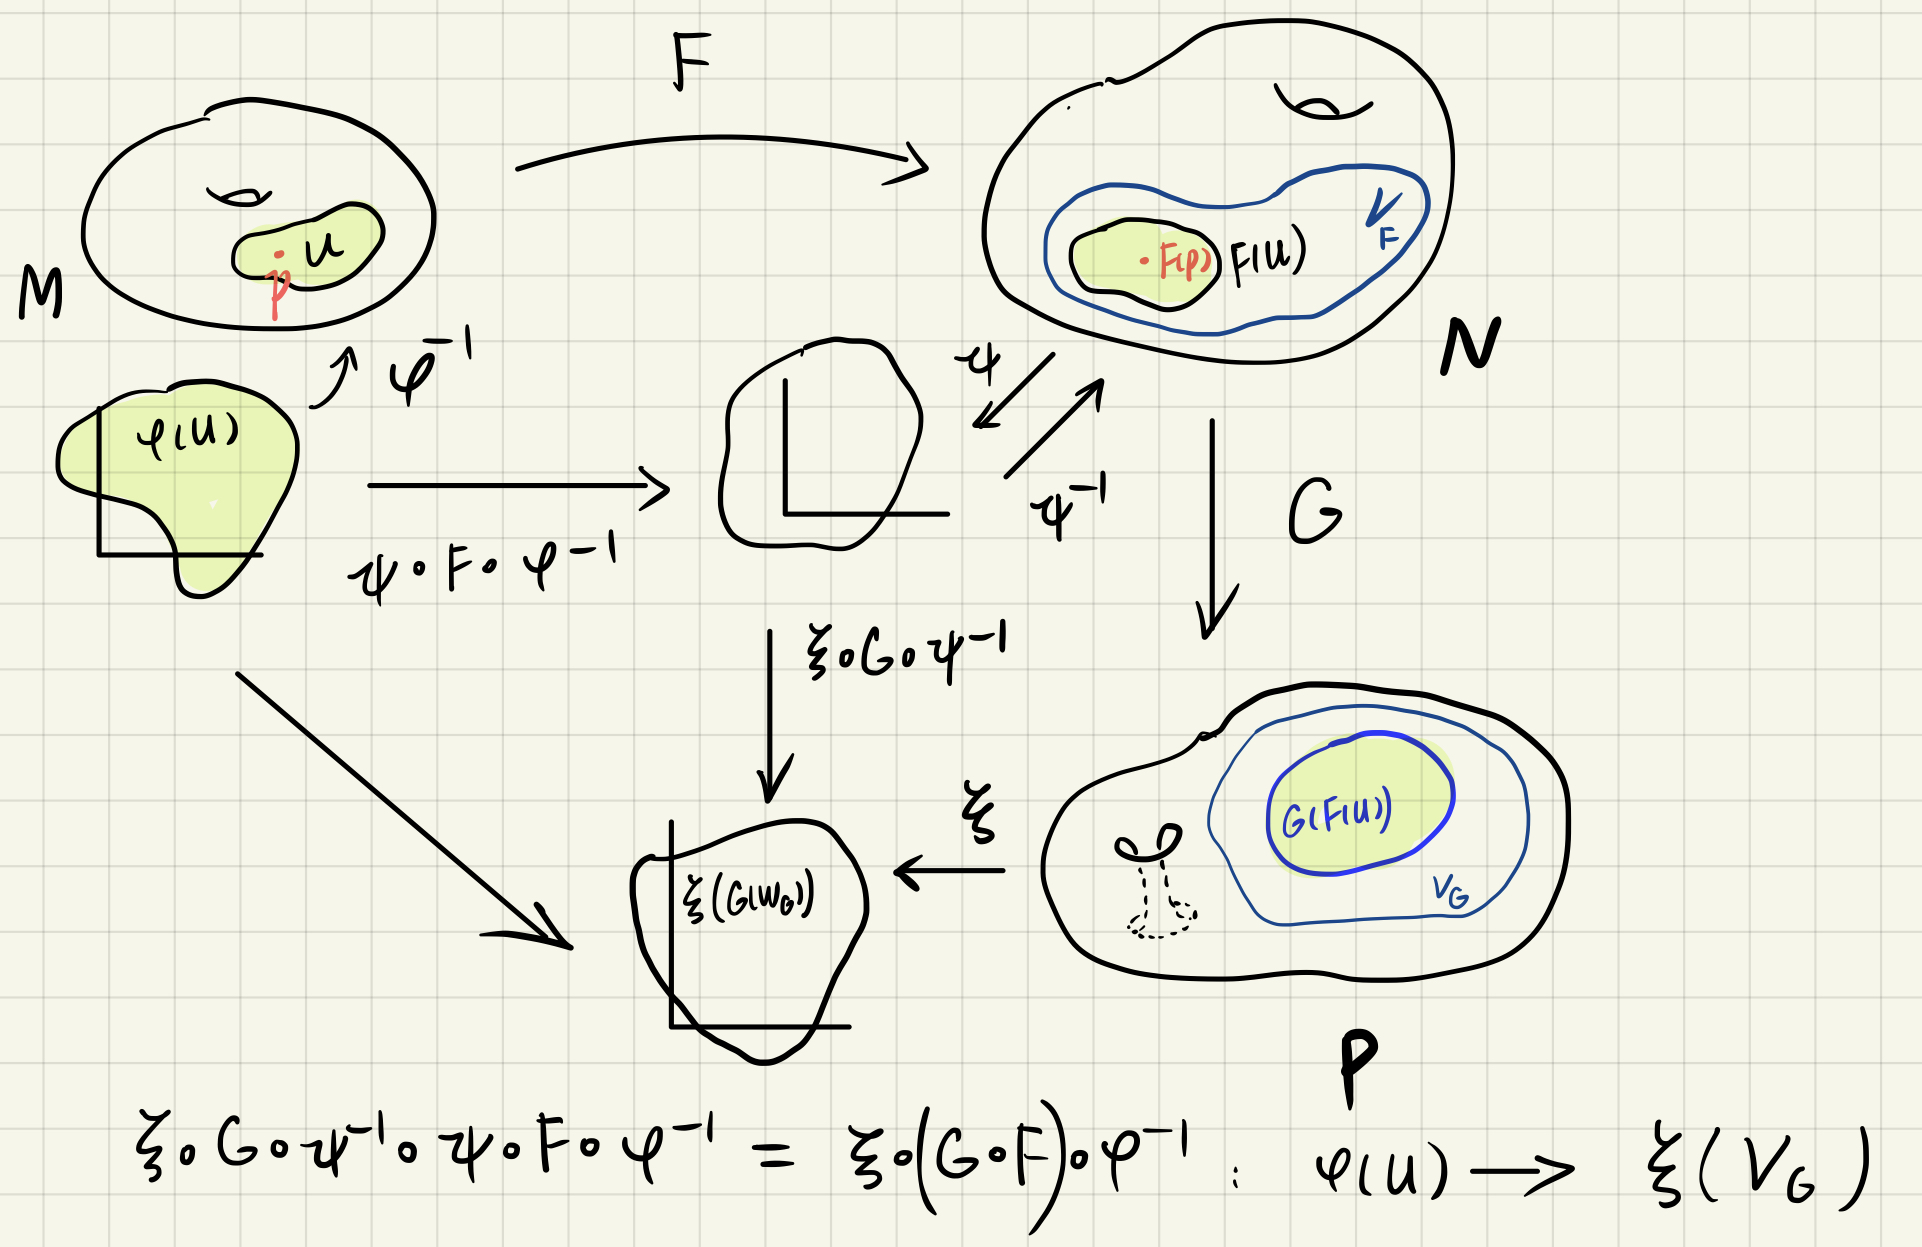
\includegraphics[scale=0.2]{figure/Lee2.15.jpeg}
    \end{figure}
    
    \item Let $p \in M$, then there are smooth charts $(U_F, \phe_F), (U_G, \phe_G)$ and $(V_F, \psi_F), (V_G, \psi_G)$ such that 
    \begin{itemize}
        \item $p \in U_f, p \in U_G$ and $F(p) \in V_F, G(p) \in V_G$,
        \item $\psi_F \circ F \circ \phe_F^{-1}$ and $\psi_G \circ G \circ \phe_G^{-1}$ are smooth functions. 
    \end{itemize}
    % 什么是product of diffeomorphisms???
    \item Let $M, N, P$ be smooth manifolds. 
    \begin{itemize}
        \item $M$ is clearly diffeomorphic with $M$ via the identity map. 
        \item If $F:M \to N$ is a diffeomorphism, so is $F^{-1}: N \to M$. 
        \item Suppose $M \simeq N$ and $N \simeq P$. Since composition of diffeomorphisms is a diffeomorphism, $M \simeq P$.
    \end{itemize}
    \end{enumerate} \qed 
\end{proof}

\section{Partitions of Unity}
\begin{lemma}
    The function $f:\R \to \R$ given by 
    $$f(t) = \begin{cases}
    e^{-1/t}, &t > 0, \\
    0,        &t \leq 0, \end{cases}$$
    is smooth. 
\end{lemma}
\begin{proof}
    This is a calculus exercise. \qed 
\end{proof}
\begin{lemma}
    For any $0 < r_1 < r_2$ there is a smooth functions $h: \R^n \to \R$, where 
    \begin{enumerate}
    \item $H = 1$ on $\cl{B_{r_1}(0)}$;
    \item $0<H<1$ on $B_{r_2}(0) \setminus \cl{B_{r_1}(0)}$;
    \item $H = 0$ on $\R^n \setminus B_{r_2}(0)$.
    \end{enumerate}
    Using the notation in Urysohn's lemma, we can write 
    $$\cl{B_{r_1}(0)} \prec h \prec B_{r_2}(0). $$
\end{lemma}
\begin{proof}
    Let  $$f(t) = \begin{cases}
    e^{-1/t}, &t > 0, \\
    0,        &t \leq 0, \end{cases}$$
    and define 
    $$ H(x) = \frac{f(r_2 - |x|)}{f(r_2 - |x|) + f(|x| - r_1)}. $$
    Then
    \begin{enumerate}
    \item If $x \in \cl{B_{r_1}(0)}$, then $0 \leq |x| \leq r_1 < r_2$, so
    $f(|x|-r_1) = 0$, hence $H(x) = f(r_2-|x|) / f(r_2-|x|) = 1$.
    \item Let $x \in B_{r_2}(0) \setminus \cl{B_{r_1}(0)}$, then $r_1 < |x| < r_2$, so $f(r_2 - |x|) > 0$ and $f(|x|-r_1) > 0$, hence $0 < H(x) < 1$.
    \item If $x \in \R^n \setminus B_{r_2}(0)$, then $|x| \geq r_2$, so $f(r_2 - |x|) = 0$.
    \end{enumerate}
    Therefore $H$ is as desired. \qed 
\end{proof}

\begin{definition}
    Let $M$ be a topological space, $\calX=(X_\a)_{\a \in A}$ be an open cover of $M$. A \textbf{partition of unity} subordinate to $\calX$ is a family $\{\psi_\a\}_{\a \in A}$ of continuous functions $\psi_\a:M \to \R$ with the following properties:
    \begin{enumerate}
    \item $0 \leq \psi_\a(x) \leq 1 ~\forall \a \in A$ and $\forall x \in M$.
    \item $\supp (\psi_\a) \subset X_\a$ for each $\a \in A$. 
    \item $\{\supp (\psi_\a)\}_{\a \in A}$ is locally finite.
    \item $\sum_{\a \in A} \psi_\a(x) = 1$ for all $x \in M$. 
    \end{enumerate}
    If $M$ is a smooth manifold and each $\psi_\a$ is smooth, then $\{\psi_\a\}_{\a \in A}$ is called a smooth partition of unity. 
\end{definition}

\begin{theorem}\label{Lee2.23}
    Suppose $M$ is a smooth manifold and $\calX = (X_\a)_{\a \in A}$ is an open cover of $M$. Then there exists a smooth partition of unity subordinate to $\calX$. 
\end{theorem}

If $M$ is a topological space, $A \subset M$ is a closed set, $U \supset A$ is open, a continuous function $\psi:M \to \R$ is called a \textbf{bump function} for $A$ supported in $U$ if $\psi = 1$ on $A$, $\supp \psi \subset U$, and $0 \leq \psi \leq 1$. Analysts use the notation $A \prec f \prec U$ to describe the above properties. 
\begin{proposition}\label{Lee2.25}
    Let $M$ be a smooth manifold. For any closed $A \subset M$ and any open $U \supset A$, there exists a smooth bump function for $A$ supported in $U$. 
\end{proposition}
\begin{proof}
    Let $U_0 = U$ and $U_1 = M \setminus A$, and let $\{\psi_0, \psi_1\}$ be a smooth partition of unity subordinate to the open cover $\{U_0, U_1\}$. Since $\psi_0 = 0$ on $A$, it follows that $\psi_0 = \sum_i \psi_i = 1$ there, the function $\psi_0$ has the desired properties. \qed 
\end{proof}
\begin{lemma}[extension lemma]
    Suppose $M$ is a smooth manifold, $A \subset M$ is closed, $f:A \to \R^k$ is a smooth function. Then for any open $U \supset A$, there is a smooth function $\Tilde{f}:M \to \R^k$ such that $\Tilde{f}|_A = f$ and $\supp \Tilde{f} \subset U$. 
\end{lemma}

% input in smoothness.tex

\section{Manifolds with Boundary}
We define the \textbf{closed $n$-dimensional upper half-space} $\H^n = \{(x^1, \cdots, x^n) \in \R^n: x^n \geq 0\}$. When $n>0$, the interior and boundary of $\H^n$ are given by 
\begin{align*}
    \Int \H^n &= \{(x^1, \cdots, x^n) \in \R^n: x^n > 0\},       \\
    \partial \H^n &= \{(x^1, \cdots, x^n) \in \R^n: x^n = 0\}.
\end{align*}
In the $n=0$ case, $\H^0 = \R^0 = \{0\}$, so $\Int H^0 = \R^0$ and $\partial \H^0 = \varnothing$. 
    %% input in smoothness.tex

\section{Manifolds with Boundary}
We define the \textbf{closed $n$-dimensional upper half-space} $\H^n = \{(x^1, \cdots, x^n) \in \R^n: x^n \geq 0\}$. When $n>0$, the interior and boundary of $\H^n$ are given by 
\begin{align*}
    \Int \H^n &= \{(x^1, \cdots, x^n) \in \R^n: x^n > 0\},       \\
    \partial \H^n &= \{(x^1, \cdots, x^n) \in \R^n: x^n = 0\}.
\end{align*}
In the $n=0$ case, $\H^0 = \R^0 = \{0\}$, so $\Int H^0 = \R^0$ and $\partial \H^0 = \varnothing$. 

\chapter{Tangent Spaces}
    \section{Tangent Vectors}
\subsection{Geometric Tangent Vectors}
In $\R^n$, we always identify a \textbf{point} with a \textbf{vector}, expressed by the coordinates $(x^1,\cdots,x^n)$. However, when come to tangent vectors, it is convenient to think of a point as a location, and think of a vector as have magnitude and direction. 

Let us begin with a prototype definition of tangent vectors in Euclidean space. 
Given a point $a \in \R^n$, define the \textbf{geometric tangent space} to $\R^n$ at $a$, denoted by $\R_a^n$, to be the set 
$$\{(a,v): v \in \R^n\} = \{a\} \times \R^n. $$
A \textbf{geometric tangent vector} in $\R^n$ is an element of $\R_a^n$ for some $a \in \R^n$. We abbreviate $(a,v)$ as $v_a$ and think of $v_a$ as the vector $v$ with its initial point at $a$. These definitions will serve as prototypes of tangent spaces on a manifold. So far they are of no practical uses because there is nothing to ``tangent" $\R^n$! \\
\begin{remark}
    We can regard a geometric tangent vector as a special type of vector which is not unique up to translation. Two \textit{vectors} are identical if they have the same direction and magnitude, but two \textit{geometric tangent vectors} are distinct even if 
    \begin{itemize}
    \item their initial points are different, and
    \item they have the same direction and magnitude.
    \end{itemize}
\end{remark}

\begin{example}[~(directional derivatives)]
    Any geometric tangent vector $v_a \in \R_a^n$ yields a map 
    \begin{align*}
    &D_v|_a: C^\infty(\R^n) \to \R \\
    &D_v|_a f = D_v f(a) = \dv{}{t}\bigg|_{t=0} f(a+tv).
    \end{align*}
    This operation is linear over $\R$ and satisfies the Leibniz's rule:
    $$D_v|_a(fg) = f(a)D_v|_a g + g(a) D_v |_a f. $$
    If $v_a = v^i e_i|_a$ in terms of the standard basis, then by the chain rule we have 
    \begin{align*}
    D_v|_a f &= \dv{}{t}\bigg|_{t=0} f(a_1+t v^1, \cdots, a_n+t v^n) 
    = v^i {\pdv{f}{x^i}}(a), 
    \end{align*}
    where we are using the summation convention.
\end{example}
\begin{definition}
    If $a$ is a point of $\R^n$, a map $w: C^\infty(\R^n) \to \R$ is called a \textbf{derivation} at $a$ if is linear over $\R$ and satsifies the \textbf{Leibniz's rule}:
    $$w(fg) = f(a) w(g) + g(a) w(f). $$
    Denote the set of all derivations of $C^\infty(\R^n)$ at $a$ by $T_a \R^n$.
\end{definition}
\begin{lemma}
    Let $a \in \R^n, w \in T_a \R^n$, and $f,g \in C^\infty(\R^n)$.
    \begin{enumerate}
    \item If $f$ is a constant function, then $wf = 0$.
    \item If $f(a) = g(a) = 0$, then $w(fg) = 0$.
    \end{enumerate}
\end{lemma}
\begin{proof}
    If $f_1=1$, then $wf_1 = w(f_1f_1) = f_1(a)wf_1 + (wf_1)f_1(a) = 2wf_1$, hence $wf_1 = 0$. If $f=c$, then by linearity $wf = w(cf_1) = cwf_1 = 0$. 
    If $f(a) = g(a) = 0$, then by the Leibniz's rule $w(fg) = 0$. \qed 
\end{proof}
\begin{proposition}[$\R_a^n \simeq T_a\R^n$]
    Let $a \in \R^n$.
    \begin{enumerate}
    \item For each gemoetric tangent vector $v_a \in \R_a^n$, the map
    \begin{align*}
    &D_v|_a: C^\infty(\R^n) \to \R \\
    &D_v|_a f = D_v f(a) = \dv{}{t}\bigg|_{t=0} f(a+tv).
    \end{align*}
    is a derivation at $a$. 
    \item The map $v_a \mapsto D_v|_a$ is an isomorphism from $\R_a^n$ to $T_a\R^n$.
    \item The $n$ partial derivative operators 
    $$\pdv{}{x^1}\bigg|_a, \cdots, \pdv{}{x^n}\bigg|_a$$
    form a basis for $T_a \R^n$. 
    \end{enumerate}
\end{proposition}
\begin{proof}
    The directional derivative operator is the same as the differentiation in calculus, so $\D_v|_a$ is clearly a derivation. Now we show that $\R_a^n \simeq T_a \R^n$. Write $u = u^i e_i|_a, v = v^i e_i|_a$ in terms of the standard basis, then 
    $$D_{u+v}|_a(f) = (u^i+v^i){\pdv{f}{x^i}}(a) = u^i{\pdv{f}{x^i}}(a) + v^i{\pdv{f}{x^i}}(a) = D_u|_a(f) + D_v|_a(f), $$
    and $D_u|_a(cf) = cD_u|_a(f)$ is easy to see. This shows the linearity. 

    Denote the map by $T: v_a \mapsto Tv_a = D_v|_a$. To see that $T$ is injective, suppose $Tv_a = D_v|_a = 0$, then take $f$ to be the $j$th coordinate function: $f(x^1, \cdots, x^j, \cdots, x^n) = x^j$, we obtain
    $$0 = D_v|_a(f) = v^i {\pdv{f}{x^i}}(f)\bigg| = v^j. $$
    Since this is true for each $j$, it follows that $v_a$ is the zero vector. 

    Now we show the surjectivity. Let $w \in T_a\R^n$ be arbitrary, and define $v = v^i e_i$, where the coefficients $v^1, \cdots, v^n$ are given by 
    $v^i = w(x^i)$. Here $x^i$ is the $i$th coordinate function: $(x^1,\cdots,x^i,\cdots,x^n) \mapsto x^i$. We will show that $w = D_v|_a$.
    Let $f$ be any smooth real-valued function on $\R^n$. By Taylor's theorem, we can write
    \begin{align*}
    f(x)=f(a) + \Sum{i=1}{n}{\pdv{f}{x^i}}(a)(x^i-a^i) + \Sum{i,j=1}{n}(x^i-a^i)(x^j-a^j)\int_0^1 (1-t){\pdv[2]{f}{x^i}{x^j}} (a+t(x-a))~dt.
    \end{align*}
    Each term in the last sum is a product of two smooth functions of $x$ that vanish at $x=a$. Thus 
    \begin{align*}
    wf &= w(f(a)) + \Sum{i=1}{n} w\br{{\pdv{f}{x^i}}(a)(x^i-a^i)} \\
    &= 0 + \Sum{i=1}{n} {\pdv{f}{x^i}}(a)(w(x^i)-w(a^i)) \\
    &= \Sum{i=1}{n} {\pdv{f}{x^i}}(a)v^i = D_v|_a f. 
    \end{align*} \qed 
\end{proof}  

\subsection{Tangent Vectors on Manifolds}
\begin{definition}
    Let $M$ be a smooth manifold, and let $p \in M$. A linear map $v:C^\infty(M) \to \R$ is called a \textbf{derivation} at $p$ if it satisfies
    $$v(fg) = f(p)vg + g(p)vf \quad \forall f,g \in C^\infty(M). $$
    Denote the set of all derivations of $C^\infty(M)$ at $p$ by $T_p M$, which is a vector space called the \textbf{tangent space} to $M$ at $p$. 
    An element of $T_p M$ is called a tangent vector at $p$.
\end{definition}
\begin{lemma}
    Suppose $M$ is a smooth manifold, $p \in M, v \in T_pM$, and $f,g \in C^\infty(M)$. 
    \begin{enumerate}
    \item If $f$ is a constant function, then $vf = 0$.
    \item If $f(p) = g(p) = 0$, then $v(fg) = 0$.
    \end{enumerate}
\end{lemma}
\begin{proof}
    First let $f_1 = 1$, then $vf_1 = v(f_1 f_1) = f_1(p)vf_1 + (vf_1) f_1(p) 
    = 2vf_1$, hence $vf_1 = 0$. 
    If $f=c$, then by linearity $vf = v(cf_1) = c (vf_1) = 0$. The second assertion is obvious by the Leibniz's rule. \qed     
\end{proof}

\section{The Differential of a Smooth Map}
\begin{definition}
    If $M,N$ are smooth manifolds and $F:M \to N$ is a smooth map, for each $p \in M$ we define a map 
    \begin{align*}
    dF_p: T_pM &\to T_{F(p)}N, \\
    v &\mapsto dF_p(v),
    \end{align*}
    called the \textbf{differential} of $F$ at $p$.
    Given $v \in T_p M$, we let $dF_p(v)$ be the derivation at $F(p)$ that acts on $f \in C^\infty(N)$ by the rule
\begin{equation}
    dF_p(v)(f) = v(f \circ F). 
\end{equation}
\end{definition}
If $f \in C^\infty(N)$, then $f \circ F \in C^\infty(M)$, so $v(f \circ F)$ makes sense. The operator $dF_p(v): C^\infty(N) \to \R$ is linear since
\begin{itemize}
    \item $dF_p(v)(f+g) = v((f+g)\circ F) = v(f \circ F + g \circ F) = v(f \circ F) + v(g \circ F)$. 
    \item $dF_p(v)(cf) = v((cf) \circ F) = v(c(f\circ F)) = cv(f \circ F)$.
\end{itemize}
And $dF_p(v)$ is a derivation at $F(p)$ because 
\begin{align*}
    dF_p(v)(fg)
    &= v((fg) \circ F) = v((f\circ F)(g\circ F)) \\
    &= (f \circ F)(p) v(g \circ F) + (g \circ F)(p) v(f \circ F) \\
    &= f(F(p)) dF_p(v)(g) + g(F(p)) dF_p(v)(f). 
\end{align*}
\begin{proposition}[properties of differentials]
    Let $M,N,P$ be smooth manifolds, let $F:M \to N$ and $G:N \to P$ be smooth maps, and let $p \in M$.
    \begin{enumerate}
    \item $dF_p: T_pM \to T_{F(p)}N$ is linear.
    \item $d(G \circ F)_p = d G_{F(p)} \circ dF_p: T_p M \to T_{G \circ F(p)}P$.
    \item $d(\id_M)_p = \id_{T_pM}: T_pM \to T_pM$.
    \item If $F$ is a diffeomorphism, then $dF_p: T_pM \to T_{F(p)}N$ is an isomorphism, and $(dF_p)^{-1} = d(F^{-1})_{F(p)}$.
    \end{enumerate}
\end{proposition}
\begin{proof}
    \begin{enumerate}
    \item Let $u,v \in T_pM$ and $f \in C^\infty(N)$ be arbitrary, then 
    \begin{align*}
        dF_p(u+v)(f) = (u+v)(f \circ F) = u(f \circ F) + v(f \circ F)
        = dF_p(u)(f) + dF_p(v)(f).
    \end{align*}
    Because $f$ is arbitrary, we have $dF_p(u+v) = dF_p(u) + dF_p(v)$. Let $c$ be a scalar, then $dF_p(cu)(f) = (cu)(f \circ F) = c dF_p(u)(f)$. Therefore $dF_p$ is linear. 
    \item Let $v \in T_pM$ and $f \in C^\infty(P)$. Let $w = dF_p(v)$, and recall that 
    $dF_p:T_pM \to T_{F(p)}N$, hence $w \in T_{F(p)}N$, and 
    $dG_{F(p)}N \to T_{G(F(p))}P$. Start with
    $$(dG_{F(p)} \circ dF_p)(v) = dG_{F(p)}(dF_p(v))=dG_{F(p)}(w), $$ and then plug $f$ in the right side, 
    \begin{align*}
    dG_{F(p)}(w)(f) &= w(f \circ G) = v(f \circ G \circ F)
    = d(G \circ F)_p(v)(f). 
    \end{align*}


    
    \item Let $v \in T_pM$ and $f \in C^\infty(M)$, then 
    $$d(\id_M)_p(v)(f) = v(f \circ \id_M) = v(f), $$
    hence $d(\id_M)_p(v) = v$, implying that $d(\id_M)_p = \id_{T_pM}: T_pM \to T_pM$.
    \item First, 
    \begin{align*}
    (dF^{-1}_{F(p)} \circ dF_p)(v)(f) 
    &= dF^{-1}_{F(p)}(dF_p(v))(f) \\
    &= dF_p(v) (f \circ F^{-1}) \\
    &= v(f \circ F^{-1} \circ F) = v(f).  
    \end{align*}
    On the other hand, 
    \begin{align*}
    (dF_p \circ dF^{-1}_{F(p)})(w)(g) 
    &= dF_p(dF^{-1}_{F(p)}(w))(g) \\
    &= (dF^{-1}_{F(p)}(w))(g \circ F) \\
    &= w(g \circ F \circ F^{-1}) = w(g). 
    \end{align*}
    Therefore, $dF_p$ is invertible, and $(dF_p)^{-1}=dF^{-1}_{F(p)}$. 
    \end{enumerate} \qed 
\end{proof}
\begin{proposition}\label{Lee3.8}
    Let $M$ be a smooth manifold, $p \in M$, and $v \in T_pM$. If $f,g \in C^\infty(M)$ agree on some neighborhood of $p$, then $vf = vg$.
\end{proposition}

\begin{proposition}[the tangent space to an open submanifold]\label{Lee3.9}
    Let $M$ be a smooth manifold, let $U \subset M$ be open, and let $\iota: U \hookrightarrow M$ be the inclusion map. For every $p \in U$, the differential $d\iota_p: T_pU \to T_pM$ is an isomorphism. 
\end{proposition}
\begin{proof}
    To show injectivity, let $v \in T_pU$ and $d\iota_p(v) = 0 \in T_pM$. Let $B$ be a neighborhood of $p$ such that $\cl{B} \subset U$. Let $f \in C^\infty(U)$ be arbitrary, then the extension lemma for smooth functions implies that there exists $\Tilde{f} \in C^\infty(M)$ such that $\Tilde{f} = f$ on $\cl{B}$. Then since $f=\Tilde{f}|_U$ in a neighborhood of $p$, Proposition (\ref{Lee3.8}) implies 
    $$vf=v(\Tilde{f}|_U) = v(\Tilde{f} \circ \iota) = d\iota(v)_p (\Tilde{f}) = 0.$$
    Since this holds for every $f \in C^\infty(U)$, it follows that $v=0$, so $d\iota_p$ is injective. 

    On the other hand, suppose $w \in T_pM$ is arbitrary. Define an operator $v:C^\infty(U) \to \R$ by $vf = w\Tilde{f}$, where $\Tilde{f}$ is any smooth function on $M$ that agrees with $f$ on $\cl{B}$. By Proposition (\ref{Lee3.8}), $vf$ is independent of the choice of $\Tilde{f}$, so $v$ is well defined, and it is a derivation of $C^\infty(U)$ at $p$ because $w$ is. For any $g \in C^\infty(M)$, 
    $$d\iota_p(v)(g) = v(g \circ \iota) = w(\widetilde{g \circ \iota}) = wg, $$
    where the last two equalities follow from the facts that $g \circ \iota, \widetilde{g \circ \iota}, g$ all agree on $B$. Therefore, $d\iota_p$ is surjective. \qed 
\end{proof}
\begin{proposition}[dimension of the tangent space]
    If $M$ is an $n$-dimensional smooth manifold, then for each $p \in M$, the tangent space $T_pM$ is an $n$-dimensional vector space. 
\end{proposition}
\begin{proof}
    Given $p \in M$, let $(U,\phe)$ be a smooth coordinate chart containing $p$. Since $\phe$ is a differomorphism from $U$ to $\phe(U)$, $d\phe_p$ is an isomorphism from $T_pU$ to $T_{\phe(p)}(\phe(U))$. By Proposition (\ref{Lee3.9}), $T_pM \simeq T_pU$ and $T_{\phe(p)}\phe(U) \simeq T_{\phe(p)}\R^n$, it follows that $$\dim T_p M = \dim T_{\phe(p)}\R^n = n. $$ \qed 
\end{proof}







    \section{Computations in Coordinates}
Suppose $M$ is a smooth manifold, and let $(U,\phe)$ be a smooth coordinate chart on $M$. Then $d\phe_p: T_pM \to T_{\phe(p)}\R^n$ is an isomorphism. Since the derivations 
$\pdv*{}{x^1}|_{\phe(p)}, \cdots, \pdv*{}{x^n}|_{\phe(p)}$ form a basis for $T_{\phe(p)}\R^n$, the preimages 
$$ (d\phe_p)^{-1}\br{\pdv{}{x^1}\bigg|_{\phe(p)}}, \cdots, (d\phe_p)^{-1}\br{\pdv{}{x^n}\bigg|_{\phe(p)}} $$
form a basis for $T_pM$. We use the notation 
We use another notation $\pdv*{}{x^i}|_p$ for these vectors:
\begin{equation}\label{tan_manifold_basis}
    \pdv{}{x^i}\bigg|_p = (d\phe_p)^{-1}\br{ {\pdv{}{x^i}}\bigg|_{\phe(p)} }
  = d(\phe^{-1})_{\phe(p)}\br{{\pdv{}{x^i}}\bigg|_{\phe(p)}}.
\end{equation}
Notice that $\pdv*{}{x^i}|_{\phe(p)}$ is a derivation in $T_{\phe(p)}\R^n$, 
hence $\pdv*{}{x^i}|_{p}$ acts on a function $f \in C^\infty(U)$ by 
\begin{equation}
    \pdv{}{x^i}\bigg|_p f = d(\phe^{-1})_{\phe(p)}\br{\pdv{}{x^i}\bigg|_{\phe(p)}f }
    = \pdv{}{x^i}\bigg|_{\phe(p)}(f \circ \phe^{-1}) 
    = {\pdv{\hat{f}}{x^i}}(\hat{p}),
\end{equation}
where $\hat{f} = f \circ \phe^{-1}$ is the coordinate representation of $f$, and $\hat{p} = \phe(p)$ is the coordinate representation of $p$. We summarize these in the following prosposition. 
\begin{definition}
    The vectors $\pdv*{}{x^i}|_p$ are called the \textbf{coordinate vectors} at $p$ associated with the given coordinate system. 
\end{definition}
\begin{proposition}
    Let $M$ be a smooth $n$-manifold, $p \in M$. Then $T_pM$ is an $n$-dimensional vector space, and for any smooth chart $(U, (x^i))$ containing $p$, the coordinate vectors $\pdv*{}{x^1}|_p, \cdots, \pdv*{}{x^n}|_p$ form a basis for $T_pM$. 
\end{proposition}
Thus, a tangent vector $v \in T_pM$ can be written uniquely as a linear combination $$v = v^i \pdv{}{x^i}\bigg|_p.$$
The ordered basis $(\pdv*{}{x^i}|_p)$ is called a \textbf{coordinate basis} for $T_pM$, and the numbers $v^1, \cdots, v^n$ are called the \textbf{components} of $v$ with respect to the coordinate basis. For each $j$, the components of $v$ are given by $v^j = v(x^j)$, where $x^j$ is the $j$th coordinate function. 

\subsection{The Differential in Coordinates}
Consider a smooth map $F:U \to V$, $U \subset \R^n, V \subset \R^m$ are open 
subsets. Let $(x^1, \cdots, x^n)$ denote the coordinates in $U$ and $(y^1, \cdots, y^m)$ denote those in $V$. 
$dF_p: T_p\R^n \to T_{F(p)}\R^m$ acts on a basis vector as follows:
\begin{align*}
    dF_p \br{\pdv{}{x^i}\bigg|_p}f
    &= \pdv{}{x^i}\bigg|_p (f \circ F) = \Sum{j=1}{m}{\pdv{f}{y^j}}(F(p)){\pdv{F^j}{x^i}}(p) \\
    &= \br{\Sum{j=1}{m}{\pdv{F^j}{x^i}}(p) \pdv{}{y_j}\bigg|_{F(p)} }f \\
    &= \br{{\pdv{F^j}{x^i}}(p) \pdv{}{y_j}\bigg|_{F(p)}} f.
    \quad (\text{Einstein summation})
\end{align*}
Since $f \in C^\infty(V)$ is arbitrary, we have 
\begin{equation}\label{Lee3.9}
    dF_p \br{\pdv{}{x^i}\bigg|_p} = {\pdv{F^j}{x^i}}(p) \pdv{}{y_j}\bigg|_{F(p)}.
\end{equation}
In terms of the coordinate bases, the matrix of the linear map $dF_p:T_p\R^n \to T_{F(p)}\R^m$:
$$ {\everymath{\displaystyle}
   \begin{pmatrix} 
    {\pdv{F^1}{x^1}}(p) & \cdots & {\pdv{F^1}{x^1}}(p) \\
    \vdots              & \ddots & \vdots              \\
    {\pdv{F^1}{x^1}}(p) & \cdots & {\pdv{F^1}{x^1}}(p) 
   \end{pmatrix}}. $$
This is non other than the Jacobian matrix of $F$ at $p$. In this case, $dF_p: T_p\R^n \to T_{F(p)}\R^m$ corresponds to the \textit{total derivative} $DF(p): \R^n \to \R^m$. 

Now we consider a smooth map $F:M \to N$ between smooth manifolds. Choosing smooth coordinate charts $(U,\phe)$ for $M$ containing $p$ and $(V,\psi)$ for $N$ containing $F(p)$, we obtain the coordinate representation $\hat{F} = \psi \circ F \circ \phe^{-1}$ from a subset of $\R^n$ to $\R^m$. 
Next, we will find the domain of $\hat{F}$. Let's draw a diagram:
\begin{center}
    \begin{tikzcd}
    M \arrow[r, "F"] & N \arrow[d, "\psi"]   \\
    \R^n \arrow[u, "\phe^{-1}"] \arrow[r, "\psi \circ F \circ \phe^{-1}"] & 
    \R^m 
    \end{tikzcd}
\end{center}
But the domain of $\phe$ is $U$ and the domain of $\psi$ is $V$, so we can be a bit more precise step by step:
\begin{center}
    \begin{tikzcd}
    U \arrow[r, "F"] & V \cap F(U) \arrow[d, "\psi"]   \\
    \R^n \arrow[u, "\phe^{-1}"] \arrow[r, "\psi \circ F \circ \phe^{-1}"] & 
    \R^m 
    \end{tikzcd}    
\end{center} 
$\psi$ should take values on $V \cap F(U)$, but this also affects the domain of $F$. Instead of starting from $U$, $F$ will map from $F^{-1}(V \cap F(U)) = F^{-1}(V) \cap U$. Thus the domain of the diffeomorphism $\phe^{-1}$ is $\phe(U \cap F^{-1}(V))$, and our ultimate diagram goes:
\begin{center}
    \begin{tikzcd}
    F^{-1}(V \cap F(U)) \arrow[r, "F"] & V \cap F(U) \arrow[d, "\psi"]   \\
    \phe(U \cap F^{-1}(V)) \arrow[u, "\phe^{-1}"] \arrow[r, "\psi \circ F \circ \phe^{-1}"] & 
    \psi(V \cap F(U))
    \end{tikzcd}    
\end{center} 
Using the formula \ref{tan_manifold_basis} and chain rule, we compute 
\begin{align*}
    dF_p\br{\pdv{}{x^i}\bigg|_p}
    &= dF_p \br{d(\phe^{-1})_{\hat{p}}\br{\pdv{}{x^i}\bigg|_{\hat{p}} } } \\
    &= dF_{\phe^{-1}(\hat{p})} d(\phe^{-1})_{\hat{p}} \br{\pdv{}{x^i}\bigg|_{\hat{p}} } \\
    &= d(F \circ \phe^{-1})_{\hat{p}} \br{\pdv{}{x^i}\bigg|_{\hat{p}} } 
     = d(\psi^{-1} \circ \hat{F})_{\hat{p}} \br{\pdv{}{x^i}\bigg|_{\hat{p}} } \\
    &= d(\psi^{-1})_{\hat{F}(\hat{p})}\br{d\hat{F}_{\hat{p}} \left(\pdv{}{x^i}\bigg|_{\hat{p}} \right) } \quad (\text{chain rule}) \\
    &= d(\psi^{-1})_{\hat{F}(\hat{p})} \br{  {\pdv{\hat{F}^j}{x^i}}(\hat{p}) \pdv{}{y^j}\bigg|_{\hat{F}(\hat{p})}  } \quad (\hat{F}(\hat{p}) = F(p)) \\
    &= (d\psi_{F(p)})^{-1} \br{  {\pdv{\hat{F}^j}}{x^i}(\hat{p}) \pdv{}{y^j}\bigg|_{\hat{F}(\hat{p})}  } \quad (\ref{tan_manifold_basis}) \\
    &= {\pdv{\hat{F}^j}{x^i}} (\hat{p}) \pdv{}{y^j} \bigg|_{F(p)}.
\end{align*}

\subsection{Change of Coordinates}
Let $(U,\phe), (V,\psi)$ be two smooth charts on $M$, and $p \in U \cap V$. Denote the coordinate functions of $\phe$ by $(x^i)$ and those of $\psi$ by $(\tilde{x}^i)$.
Any tangent vector at $p$ can be represented by either basis $\displaystyle{\br{\pdv{}{x^i}\bigg|_p}}$ or $\displaystyle{\br{\pdv{}{\tilde{x}^i}\bigg|_p}}$.

Write the transition map $\psi \circ \phe^{-1}: \phe(U \cap V) \to \psi(U \cap V)$ in the following notation:
%$$\psi \circ \phe^{-1}(x) = (\tilde{x}^1(x), \cdots, \tilde{x}^n(x)) \quad (x \in \phe(U \cap V)). $$
$$\psi \circ \phe^{-1}(x) = (y^1(x), \cdots, y^n(x)) \quad (x \in \phe(U \cap V)). $$
By (\ref{Lee3.9}), we have 
%\begin{align*}
    %d(\psi \circ \phe^{-1})_{\phe(p)}\br{ \pdv{}{x^i}\bigg|_{\phe(p)} }
    %&= \pdv{\Tilde{x}^j}{x^i}(\phe(p))\br{ \pdv{}{\tilde{x}^i}\bigg|_{\psi(p)} }.
%\end{align*}
\begin{align*}
    d(\psi \circ \phe^{-1})_{\phe(p)}\br{ \pdv{}{x^i}\bigg|_{\phe(p)} }
    &= {\pdv{\Tilde{x}^j}{x^i}} (\phe(p))  \pdv{}{y^i}\bigg|_{\psi(p)} .
\end{align*}
Using the definition of coordinate vectors, we obtain
\begin{align*}
    \br{\pdv{}{x^i}\bigg|_p}
    &= d(\phe^{-1})_{\phe(p)}\br{ \pdv{}{x^i}\bigg|_{\phe(p)} } \\
    &= d(\psi^{-1} \circ \psi \circ \phe^{-1})_{\phe(p)} \br{ \pdv{}{x^i}\bigg|_{\phe(p)} } \\
    &= d(\psi^{-1})_{(\psi \circ \phe^{-1})(\phe(p))} \circ d(\psi \circ \phe^{-1})_{\phe(p)} \br{ \pdv{}{x^i}\bigg|_{\phe(p)} } \\
    &= d(\psi^{-1})_{\psi(p)} \br{  {\pdv{y^j}{x^i}} (\phe(p)) \pdv{}{y^i}\bigg|_{\psi(p)}  } \\
    &= {\pdv{y^j}{x^i}}(\hat{p}) \pdv{}{\tilde{x}^j}\bigg|_p,
\end{align*}
where $\hat{p} = \phe(p)$.
Applying this to the components of a derivation $\displaystyle{v = v^i \pdv{}{x^i}\bigg|_p = \Tilde{v}^j\pdv{}{\Tilde{x}^j}\bigg|_p }$, by the above rule
$$\Tilde{v}^j = {\pdv{y^j}{x^i}}(\hat{p})v^i, $$
where $y^j$'s are the components of the transition map $\psi \circ \phe^{-1}$.
\begin{example} 
    The transition map between polar coordinates and standard coordinates in suitable open subsets of $\R^2$ is given by $(x,y) = (r\cos \cta, r\sin \cta)$. Let $p \in \R^2$ with polar coordinate represent being $(r,\cta) = (2, \pi/2)$, and $v \in T_p\R^2$ with polar coordinate represent being
    $$ v = 3 \dvBase{r}{p}-\dvBase{\cta}{p}. $$ 
    We find
    \begin{align*}
    &\dvBase{r}{p} = \pdv{(r\cos \cta)}{r}\bigg|_{(2,\pi/2)} \dvBase{x}{p} + 
                    \pdv{(r\sin \cta)}{r}\bigg|_{(2,\pi/2)} \dvBase{y}{p}
                  = \cos(\pi/2) \dvBase{x}{p} + \sin(\pi/2) \dvBase{y}{p} 
                  = \dvBase{y}{p}, \\
    &\dvBase{\cta}{p} = \pdv{(r\cos \cta)}{\cta}\bigg|_{(2,\pi/2)} \dvBase{x}{p} + 
                    \pdv{(r\sin \cta)}{\cta}\bigg|_{(2,\pi/2)} \dvBase{y}{p}
                  = -2\sin(\pi/2) \dvBase{x}{p} + 2\cos(\pi/2) -2\dvBase{x}{p} 
                  = \dvBase{y}{p},               
    \end{align*}
    thus $v$ has the coordinate representation in standard coodinates
    $$v = 3\dvBase{y}{p} + 2 \dvBase{x}{p}. $$
\end{example}
\begin{exercise}
    Let $(x,y)$ denote the standard coordinates on $\R^2$. Verify that $(\Tilde{x},\Tilde{y})$ are global smooth coordinates on $\R^2$, where 
    $$\Tilde{x} = x, \quad \Tilde{y} = y+x^3. $$
    Let $p = (0,1) \in \R^2$ (in standarad coordinates), and show that 
    $$ \dvBase{x}{p} \neq  \dvBase{\Tilde{x}}{p}. $$
\end{exercise}


    \section{The Tangent Bundle}
\begin{definition}
Given a smooth manifold $M$, we define the \textbf{tangent bundle} of $M$, denoted by $TM$, to be the disjoint union of the tangent spaces at all points of $M$:
$$ TM = \bigsqcup_{p \in M}T_pM. $$
\end{definition}
We often write an element of $TM$ as $(p,v)$, where $p \in M$ and $v \in T_pM$. The next proposition gives a smooth structure on $TM$, with the idea of divide-and-conquer: utilizing the smooth structure on $M$ and identifying $T_pM$ with $\R^n$. 
\begin{proposition}
    For any smooth $n$-manifold $M$, the tangent bundle $TM$ has a natural topology and smooth structure that make it into a $2n$-dimensional smooth manifold. With respect to this structure, the projection $\pi: TM \to M$ is smooth.
\end{proposition}
\begin{proof}
    Let $(U,\phe)$ be a smooth chart for $M$, then $\pi^{-1}(U)$ is an open subset of $TM$ consisting of all tangent vectors at each point of $U$. We construct a smooth structure on $TM$. Let $\phe = (x^1, \cdots, x^n)$ be the coordinate representation, and define
    $\widetilde{\phe}: \pi^{-1}(U) \to \R^{2n}$ by 
    $$ \widetilde{\phe}\br{v^i \pdv{}{x^i}\bigg|_p} = 
    (x^1(p), \cdots, x^n(p), v^1, \cdots, v^n) = (\phe(p), v), $$
    then $\{(\pi^{-1}(U), \widetilde{\phe}): (U,\phe) \text{ is a smooth chart for }M\}$ is a smooth structure on $TM$. \qed 
\end{proof}

    \section{Velocity Vectors of Curves}
% curve in manifolds
Every element in the tangent space is the velocity of some curve. This insight will be frequently used in Chapter \ref{curve and flow}: Integral Curves and Flows. 


\begin{definition}
    A \textit{curve} in $M$ is a continuous map $\ga:J \to M$, where $J$ is an interval. 
\end{definition}
Given a smooth curve $\ga: J \to M$ and $t_0 \in J$, we define the \textit{velocity} of $\ga$ at $t_0$ to be the vector
$$\ga'(t_0) = d\ga \br{\dv{}{t}\bigg|_{t_0} } \in T_{\ga(t_0)M }. $$
Here $d\ga: T_{t_0}J \to T_{\ga(t_0)}M$, and for any $f \in C^\infty(M)$, 
$$d\ga \br{\dv{}{t}\bigg|_{t_0} }(f) = \dv{}{t}\bigg|_{t_0}(f \circ \ga)(t) = (f \circ \ga)'(t_0). $$
Other common notations are
$$\dot{\ga}(t_0) = \dv{\ga}{t}(t_0) = \dv{\ga}{t}\bigg|_{t=t_0}. $$
$\ga'(t_0)$ is the derivation at $\ga(t_0)$ obtained by taking the derivative of a function along $\ga$. 

Let $(U,\phe)$ be a smooth chart with coordinate $(x^i)$. If $\ga(t_0) \in U$, we can write the coordinate representation of $\ga$ is 
$$ \widehat{\ga}(t) = (\ga^1(t), \cdots, \ga^n(t)) \in U \subset \R^n, $$ 
for $t$ sufficiently close to $t_0$. Then the coordinate formula for the differential yields
$$ \ga'(t_0) = {\dv{\widehat{\ga}^i}{t}}(t_0) \dvBase{x^i}{\ga(t_0)}. $$

Every tangent vector on a manifold is the velocity of some curve.
\begin{proposition}
    Suppose $M$ is a smooth manifold and $p \in M$. Every $v \in T_pM$ is the velocity of some smooth curve in $M$. 
\end{proposition}
\begin{proof}
    Let $(U,\phe)$ be a smooth chart centered at $p$, and write $v = v^i \pdv*{}{x^i}|_p$. For small $\eps > 0$ let $\ga:(-\eps,\eps) \to U$ be the curve whose coordinate representation is $\widehat{\ga}(t) = (tv^1, \cdots, tv^n) \in \R^n$. Hence $\ga(t) = \phe^{-1} \circ \widehat{\ga} (t) = \phe^{-1}(tv^1, \cdots, tv^n)$. Then $\ga$ is smooth and 
    \begin{itemize}
        \item $\ga(0) = \phe^{-1}(0) = p$, 
        \item $\displaystyle{ \ga'(0) = {\dv{\widehat{\ga}^i}{t}}(0) \dvBase{x^i}{\ga_0} = v^i \dvBase{x^i}{p} = v}$.    
    \end{itemize}
\end{proof}
\begin{proposition}[the velocity of a composite curve]
    Let $F:M \to N$ be a smooth map, and let $\ga:J \to M$ be a smooth curve. For any $t_0 \in J$, the velocity at $t=t_0$ of the curve $F \circ \ga:J \to N$ is given by $$(F \circ \ga)'(t_0) = dF(\ga'(t_0)). $$
\end{proposition}
Since every derivation $v \in T_p M$ is the velocity of some curve, we can compute $dF_p(v)$ by choosing a smooth curve $\ga$ whose initial tangent vector is $v$.
\begin{proposition}[computing differential using velocity]
    Suppose $F:M \to N$ is a smooth map, $p \in M$, $v \in T_pM$. Then 
    $$ dF_p(v) = (F \circ \ga)'(0), $$
    for any smooth curve $\ga:J \to M$ such that $0 \in J, \ga(0) = p, \ga'(0) = v$. 
\end{proposition}
    \section{Categories and Functors}
a \textbf{Category} $\sfC$ consists of the following things:
\begin{itemize}
    \item a class $\Ob(\sfC)$, whose elements are called \textbf{objects} of $\sfC$,
    \item a class $\Hom(\sfC)$, whose elements are called \textbf{morphisms} of $\sfC$,
    \item for each morphism $f \in \Hom(\sfC)$, two objects $X,Y \in \Ob(\sfC)$ called the \textbf{source} and \textbf{target} of $f$, respectively,
    \item for each triple $X,Y,Z \in \Ob(\sfC)$, a mapping called \textbf{composition}:
    $$\Hom_\sfC(X,Y) \times \Hom_\sfC(Y,Z) \to \Hom_\sfC(X,Z), $$
    written $(f,g) \mapsto g \circ f$. $\Hom_\sfC(X,Y)$ denotes the class of all morphisms with source $X$ and target $Y$.
\end{itemize}
The morphisms are required to satisfy the following axioms:
\begin{enumerate}
    \item \textit{Associativity}: $(f \circ g) \circ h = f \circ (g \circ h)$. 
    \item \textit{Existence of identities}: For each object $X \in \Ob(\sfC)$, there exists an \textbf{identity morphism} $\id_X \in \Hom_\sfC(X,X)$ such that 
    $\id_Y \circ f = f = f \circ \id_X$ for all $f \in \Hom_\sfC(X,Y)$. 
\end{enumerate}
    
\chapter{Submersions, Immersions, Embeddings}
    \section{Maps of Constant Rank}
Suppose $M,N$ are smooth manifolds. Given a smooth amp $F:M \to N$ and a point $p \in M$, we define the \textbf{rank} of $F$ at $p$ to be the rank of the linear map $dF_p:T_pM \to T_{F(p)}N$. If $F$ has the same rank $r$ at every point, we say that it has \textbf{constant rank}, and write $\rank F = r$. 
By the rank-nullity theorem, $\rank F \leq \min(\dim M, \dim N)$. If the rank of $dF_p$ is equal to this upper bound, we say that $F$ has \textbf{full rank} at $p$, and if $F$ has full rank everywhere, we say $F$ has full rank. 
\begin{definition}[submersion, immersion]
    A smooth map $F:M \to N$ is called a \textbf{smooth submersion} if its differential is surjective at each point (or equivalently, if $\rank F = \dim N$). It is called a \textbf{smooth immersion} if its differential is injective at each point (equivalently, $\rank F = \dim M$). 
\end{definition}

\begin{example}[~(open submanifolds)]
    Let $U$ be an open set in $\R^n$, then $U$ is a topological $n$-manifold, and the single chart $(U,\id_U)$ defines a smooth structure on $U$. 
    More generally, let $M$ be a smooth $n$-manifold and let $U \subset M$ be any open subset. Define an atlas on $U$ by 
    $$\calA_U = \{\text{smooth charts }(V,\phe)\text{ for }M\text{ such that }V \subset U\}.$$
    
    
\end{example}
\begin{example}[~(general linear group)]
    The general linear group $\mathrm{GL}(n,\R)=\{A \in \R^{n \times n}: \det A \neq 0 \}$. Show that it is an open subset of $\R^{n \times n}$, hence it is a smooth $n^2$-dimensional manifold.  
\end{example}
\begin{proof}
    
\end{proof}
\begin{example}[~(matrices of full rank)]
    Suppose $m<n$, and let $\calM_m(m \times n, \R)$ be the subset of $\calM(m \times n, \R)$ consisting of matrices of rank $m$. Prove that $\calM_m(m \times n, \R)$ is an open subset of $\calM(m \times n, \R)$, and therefore is a smooth $mn$-manifold. 
\end{example}

\begin{proposition}
    Suppose $F:M \to N$ is a smooth map and $p \in M$. If $dF_p$ is surjective, then $p$ has a neighborhood $U$ such that $F|_U$ is a submersion. 
    if $dF_p$ is injective, then $p$ has a neighborhood such that $F|_U$ is an immersion. 
\end{proposition}

\subsection{Local Diffeomorphisms}
A smooth map $F:M \to N$ is called a \textbf{local diffeomorphism} if every $p \in M$ has an open neighborhood $U$ where $F(U)$ is open and $F|_U:U \to F(U)$ is a diffeomorphism. 
\begin{example}
    The map $f:\R \to \S^1$ given by $f(t) = (\cos t, \sin t)$ is a local diffeomorphism. 
\end{example}
\begin{theorem}[inverse function theorem]
    Suppose $F:M \to N$ is a smooth map. If $p \in M$ and $dF_p$ is invertible, then there are connected open neighborhoods $U_0$ of $p$ and $V_0$ of $F(p)$ such that $F|_{U_0}: U_0 \to V_0$ is a diffeomorphism. 
\end{theorem}
\begin{proof}
    Since $dF_p$ is invertible, $n = \dim M = \dim N$. Fix charts $(U,\phe), (V,\psi)$ centered at $p$ and $F(p)$ with $F(U) \subset V$. Let 
    $$\hat{F}: \psi \circ F \circ \phe^{-1}: \phe(U) \to \psi(V), $$ then 
    $$ d\hat{F}_0 = d\psi_{F(p)} \circ dF_p \circ d(\phe^{-1})_0 $$ is invertible. By the classical inverse function theorem there exist connected open neighborhoods $\hat{U}_0 \subset \phe(U)$ and $\hat{V}_0 \subset \psi(V)$ such that 
    $\hat{F}|_{\hat{U}_0}: \hat{U}_0 \to \hat{V}_0$ is a diffeomorphism. Then letting $U_0 = \phe^{-1}(\hat{U}_0)$ and $V_0 = \psi^{-1}(\hat{U}_0)$ completes the proof. \qed 
\end{proof}


\subsection{The Rank Theorem}
\begin{theorem}
    Suppose $F:M \to N$ is a smooth map, $\dim M = m, \dim N = n$. If $F$ has constant rank $r$ (i.e., $\rank dF_p = r$ for all $p$). then for every $p \in M$ there exist smooth charts $(U,\phe), (V,\psi)$ of $M,N$ centered at $p, F(p)$ such that $F(U) \subset V$ and 
    $$\psi \circ F \circ \phe^{-1}(x^1, \cdots, x^m) = (x^1, \cdots, x^r, 0, \cdots, 0). $$
    In particular, 
    \begin{itemize}
    \item if $F$ is a smooth submersion, then $m \geq n$ and 
    $$\psi \circ F \circ \phe^{-1}(x^1, \cdots, x^m) = (x^1, \cdots, x^n). $$
    \item If $F$ is a smooth immersion, then $m \leq n$ and 
    $$\psi \circ F \circ \phe^{-1}(x^1, \cdots, x^m) = (x^1, \cdots, x^m, 0, \cdots, 0). $$
    \end{itemize}
\end{theorem}
\begin{proof}
    Linear algebra and inverse function theorem. 
\end{proof}



\begin{theorem}[global rank theorem]
    Let $F:M \to N$ be a smooth map of constant rank. 
    \begin{enumerate}
    \item If $F$ is surjective, then $F$ is a smooth submersion.
    \item If $F$ is injective, then $F$ is a smooth immersion. 
    \item If $F$ is bijective, then $F$ is a diffeomorphism. 
    \end{enumerate}
\end{theorem}


    \section{Topology Review}
\begin{theorem}[closed map lemma]
    
\end{theorem}


\section{Embeddings}
\subsection{Topological Embeddings}
An injective contniuous map that is a homeomorphism onto its image (in the subspace topology) is called a \textbf{topological embedding}. If $f:A \to X$ is such a map, we can think of $f(A)$ as a homeomorphic copy of $A$ inside $X$. 

\begin{exercise}
    Let $X$ be a topological space and let $S$ be a subspace of $X$. Show that the inclusion $\iota:S \to X$ is a topological embedding. 
\end{exercise}

\begin{proposition}
    A continuous injective map that is either open or closed is a topological embedding.
\end{proposition}

\begin{proposition}
    A surjective topological embeddings is a homeomorphism. 
\end{proposition}

\subsection{Smooth Embeddings}
A smooth map $F:M \to N$ is called a \textbf{smooth embedding} if 
\begin{enumerate}
    \item $F$ is an immersion, 
    \item $F$ is a topological embedding: $M$ is homeomorphic to $F(M) \subset N$ in the subspace topology.  
\end{enumerate}
\begin{example}

\end{example}
    


\chapter{Submanifolds and Sard's Theorem}
    \section{Embedded Submanifolds}
An embedded submanifold of $M$ is a subset $S \subset M$ which is a topological manifold (w.r.t. the subspace topology) endowed with a smooth structure that makes the inclusion $\iota:S \to M$ a smooth embedding. 
\begin{example}
    \begin{itemize}
        \item If $U \subset M$ is open, then $U$ is an embedded submanifold.
        \item $\S^{n-1} \subset \R^n$ is an embedded submanifold. 
    \end{itemize}
\end{example}

In fact, every embedded submanifold is the image of some manifold under a smooth embedding. 

\begin{proposition}
    Suppose $F:N \to M$ is a smooth embedding, then $S=F(N)$ is a topological manifold (w.r.t. the subspace topology) and has a unique smooth structure such that 
    \begin{enumerate}
    \item $S$ is an embedded submanifold. 
    \item $F:N \to S$ is a diffeomorphism. 
    \end{enumerate}
\end{proposition}    

\begin{example}[(Slices of Product Manifolds)]
    Suppose $M$ and $N$ are smooth manifolds. For each $p \in N$, the subset $M \times \{p\}$ is an embedded submanifold of $M \times N$ diffeomorphic to $M$. 
\end{example}
\begin{proof}
    $M \times \{p\}$ is the image of the smooth embedding $x \mapsto (x,p)$. 
\end{proof}
\begin{example}[(Graph of a map)] 
    Suppose $M, N$ are smooth $m, n$-manifolds, $U \subset M$ is open, $f:U \to N$ is smooth. Then 
    $$\Ga(f) = \{(x,y) \in M \times N: x\in U, y=f(x)\}$$
    is an embedded $m$-dimensional submanifold of $M \times N$. 
\end{example}
\begin{proof}
    
\end{proof}
\subsubsection*{Slice Charts}
If $U$ is an open subset of $\R^n$ and $k \leq n$, a $k$-dimensional slice of $U$ (or a $k$-slice) is a subset of the form
$$S = \{(x^1, \cdots, x^k, x^{k+1}, \cdots, x^n) \in U: x^{k+1} = c^{k+1}, \cdots, x^n = c^n\}$$
for some constants $c^{k+1}, \cdots, c^n$. In practice, those constants are often set to be zero: $c^{k+1} = \cdots = c^n = 0$. Now we define a slice on a manifold. 
\begin{definition}
    Let $M$ be a smooth $n$-manifold, and $(U,\phe)$ be a smooth chart on $M$. If $S \subset U$ such that $\phe(S)$ is a $k$-slice of $\phe(U)$, then we say that $S$ is a $k$-slice of $U$. 
\end{definition}
\begin{definition}[local $k$-slice condition]
    Let $S \subset M$ and $k \in \N$. We say that $S$ satisfies the \textbf{local $k$-slice condition} if each point of $S$ is contained in a smooth chart $(U,\phe)$ for $M$ such that $S \cap U$ is a $k$-slice in $U$. Any such chart is called a \textbf{slice chart} for $S$ in $M$. 
\end{definition}
\begin{theorem}[local slice criterion]
    Let $M$ be a smooth $n$-manifold. If $S \subset M$ is an embedded $k$-dimensional submanifold, then $S$ satisfies the local $k$-slice condition. Conversely, if $S \subset M$ is a subset that satisfies the local $k$-slice condition, then $S$ is a $k$-dimensional topological manifold, and it has a smooth structure making it into an embedded submanifold of $M$. 
\end{theorem}

\section{Level Sets}
If $\Phi:M \to N$ is a map, the preimages $\Phi^{-1}(c)$ are called level sets. 
\begin{theorem}
    Let $\Phi:M \to N$ be a smooth map with constant rank $r$. Each level set of $\Phi$ is embedded submanifold of codimension $r$ in $M$, i.e., $\dim \Phi^{-1}(c) = \dim M - r$
\end{theorem}

Let $\Phi:M \to N$ be a smooth map. 
\begin{itemize}
    \item $p \in M$ is called a \textbf{regular point} if $d\Phi_p$ is surjective, otherwise it is called a \textbf{critical point}.
    \item $c \in N$ is called a \textbf{regular value} if every point in $\Phi^{-1}(c)$ is a regular point (in this case $\Phi^{-1}(c)$ is called a regular level set), otherwise $c$ is called a critical value. 
\end{itemize}
\begin{corollary}
    Every regular level set of a smooth map $\Phi:M \to N$ is an embedded submanifold with dimension equal to $\dim M - \dim N$. 
\end{corollary}

Every embedded submanifold is locally a level set of a smooth submersion. 
\begin{proposition}\label{5.16}
    Let $S$ be a subset of a smooth $m$-manifold $M$, then $S$ has the structure of an embedded $k$-dimensional submanifold if and only if every point in $S$ has an open neighborhood $U$ such that $U \cap S$ is a level set of a smooth submersion $\Phi:U \to \R^{m-k}$.
\end{proposition}
\begin{proof}
    First suppose $S$ is an embedded $k$-submanifold, and let $(x^1, \cdots, x^m)$ be slice coordinates for $S$ on an open subset $U \subset M$. Let $\Phi:U \to \R^{m-k}$ given in coordinates by 
    $$\Phi(x) = (x^{k+1}, \cdots, x^m). $$
    Then $\Phi$ is a smooth submersion. By the local slice condition, $S \cap U$ is a $k$-slice in $U$, so 
    $$S \cap U = \{(x^1,\cdots,x^k,x^{k+1},\cdots,x^m)\in U: x^{k+1}=c^{k+1},\cdots,x^m=c^m\},$$
    hence $S \cap U = \Phi^{-1}(c^{k+1}, \cdots, c^m)$ is a level set of $\Phi$. 

    Conversely, suppose that every $p \in S$ has a neighborhood $U$ and a smooth submersion $\Phi:U \to \R^{m-k}$ such that $S \cap U$ is a level set of $\Phi$. Then $S \cap U$ is an embedded submanifold of $U$, so it satisfies the local slice condition. It follows that $S$ itself is an embedded submanifold of $M$. 
\end{proof}
If $S \subset M$ is an embedded submanifold, a smooth map $\Phi:M \to N$ such that $S$ is a regular level set of $\Phi$ is called a \textit{defining map} for $S$. More generally, if $U$ is an open subset of $M$ and $\Phi:U \to N$ is a smooth map such that $S \cap U$ is a regular level set of $\Phi$, then $\Phi$ is called a \textit{local defining map} for $S$. The above proposition says that every embedded submanifold admits a local defining function in a neighborhood of each of its points. 
 
\subsection*{Regular Sets}
If $\Phi:M \to N$ is a smooth map, a point $p \in M$ is said to be a \textit{regular point} of $\Phi$ if $d\Phi_p:T_pM \to T_{\Phi(p)}N$ is surjective; it is called a \textit{critical point} of $\Phi$ otherwise. 

A point $c \in N$ is called a \textit{regular value} of $\Phi$ if every point in $\Phi^{-1}(c)$ is a regular point, and a \textit{critical value} otherwise. 
\begin{theorem}[regular level set theorem]
    Every regular level set of a smooth map between smooth manifolds is a properly embedded submanifold whose codimension is equal to the dimension of the codomain. 
\end{theorem}
\section{Immersed Submanifolds}

\section{The Tangent Space to a Submanifold}
\begin{proposition}[characerization of $T_pS$]
    Suppose $M$ is a smooth manifold, $S \subset M$ is an embedded submanifold, and $p \in S$. As a subspace of $T_pM$, the tangent space $T_pS$ is characterized by 
    $$T_pS = \{v \in T_pM : vf = 0 \text{ whenever }f \in C^\infty \text{ and }f|_S=0\}. $$
\end{proposition}
\begin{proposition}
    Suppose $M$ is a smooth manifold and $S \subset M$is an embedded submanifold. If $\Phi:U \to N$ is any local defining map for $S$, then 
    $$ T_pS = \ker d\Phi_p:T_pM \to T_{\Phi(p)}N $$
    for each $p \in S \cap U$. 
\end{proposition}

    \section{Sard's Theorem}

\begin{theorem}[Sard's theorem]
    Suppose $M,N$ are smooth manifolds, $F:M \to N$ is a smooth map. Then the set of critical values of $F$ has measure zero in $N$. 
\end{theorem}

\begin{corollary}
    Suppose $M,N$ are smooth manifolds, and $F:M \to N$ is a smooth map. if $\dim M < \dim N$, then $F(M)$ has measure zero in $N$. 
\end{corollary}

\section{The Whitney Embedding Theorem}

\begin{theorem}[Whitney embedding theorem]
    Every smooth $n$-manifold admits a proper smooth embedding into $\R^{2n+1}$.
\end{theorem}
\section{The Whitney Approximation Theorem}

\subsection{Tubular Neighborhoods and Normal Bundles}

\subsection{Smooth Approximation of Maps Between Manifolds}

\begin{theorem}[Whitney approximation theorem]
    Suppose $N, M$ are a smooth manifolds and $F:N \to M$ is a continuous map. Then $F$ is homotopic to a smooth map. If $F$ is smooth on a closed subset $A \subset N$, then the homotopy can be taken to be relative to $A$.    
\end{theorem}
\begin{proof}
    We embed $M$ into $\R^n$. Let $U$ be a tubular neighborhood of $M$, and $r:U \to M$ be the smooth retraction. For  $x \in M$, let 
    $$\d(x) = \sup\{\eps \leq 1:B_\eps(x) \subset U\}, $$
    then $\d:M \to \R^+$ is continuous. Let $\widetilde{\d} = \d \circ F:N \to \R^+$.
\end{proof}
\section{Transversality}
\begin{definition}
    Suppose $M$ is a smooth manifold. Two embedded submanifolds $S,S' \subset M$ are \textit{transverse} if 
    $$T_pS + T_pS' = T_p M \quad \text{for all }p \in S \cap S' $$
\end{definition}
\begin{definition}
    If $F:N \to M$ is smooth and $S \subset M$ is an embedded submanifold, then $F$ is transverse to $S$ if 
    $$T_{F(x)}S + dF_x(T_xN) = T_{F(x)}M $$ or all $x \in F^{-1}(S)$. 
\end{definition}
\begin{theorem}
    Suppose $N,M$ are smooth manifolds and $S \subset M$ is an embedded submanifold.
    \begin{enumerate}
    \item If $F:N \to M$ is transverse to $S$, then $F^{-1}(S) \subset N$ is an embedded submanifold with codimension of $F^{-1}(S)$ in $N$ equals codimension of $S$ in $M$. 
    \item If $S' \subset M$ is an embedded submanifold which is transverse to $S$, then $S' \cap S \subset M$ is an embedded submanifold with 
    $$ \codim S \cap S' = \codim S + \codim S'. $$
    \end{enumerate}
\end{theorem}
\begin{proof}
    We use the fact that a subset is a submanifold if and only if it is locally the level set of a submersion (see \textbf{Proposition \ref{5.16}}). 
    Fix $x \in F^{-1}(S)$, then there is an open neighborhood $U \subset M$ of $F(x)$ and a submersion $\phe:U \to \R^k$ ($k=\dim M - \dim S$), where $\phe^{-1}(0) = S \cap U$. Let $\widetilde{U}=F^{-1}(U)$ and $\widetilde{\phe} = \phe \circ F$, then $\widetilde{\phe}^{-1}(0) = \widetilde{U} \cap F^{-1}(S)$. 
    
    We claim that $\widetilde{\phe}$ is a submersion in a neighborhood of $x$. It suffices to show that $d\widetilde{\phe}_x:T_xN \to T_{\widetilde{\phe}(x)}\R^k$ is surjective. Fix $v \in T_{\widetilde{\phe}(x)}\R^k$, since $\phe$ is a submersion, $v = d\phe_{F(x)} w$ for some $w \in T_{F(x)}M$. Since $F$ is transverse to $S$ and $F(x) \in S$, 
    $$w = w_1 + dF_x w_2 \quad \text{for some }w_1 \in T_{F(x)}S, w_2 \in T_xN. $$
    Since $\phe = 0$ on $S$, $d\phe_{F(x)}w_1 = 0$, so 
    $$v = d\phe_{F(x)}w = d\phe_{F(x)}(w_1 + dF_x w_2) = d\phe_{F(x)}dF_x w_2 = d\widetilde{\phe}_x w_2.$$
    Apply (1) to the inclusion map $S' \hookrightarrow M$, we get (2). 
\end{proof}
\subsection*{Deforming To Obtain Transversality}
Goal: Given $F:N \to M$ smooth and $X \subset M$ embedded, "deform" $F$ to be transverse. 
\begin{theorem}\label{6.35}
    Suppose $N,M$ are smooth manifolds and $X \subset M$ is an embedded submanifold. If $F:N \times S \to M$ is smooth and transverse to $X$, then for almost every $s \in S$ the map $F_s = F(\cdot, s):N \to M$ is transverse to $X$. 
\end{theorem}
\begin{proof}
    Since $F:N \times S \to M$ is transverse to $X$, $W:=F^{-1}(X) \subset N \times S$ is an embedded submanifold. Let $\pi:N \times S \to S$ be the projection.
    By Sard's theorem it suffices to show that if $s \in S$ is a regular value of $\pi|_W$, then $F_s$  is transverse to $X$. 

    Fix $p \in F_s^{-1}(X)$ and $v \in T_{F_s(p)}M$, let $q = F_s(p) = F(p,s)$. By transversality, 
    $$v = u+dF_{(p,s)}(v_1, v_2)$$
    for some $u \in T_qX$ and $(v_1,v_2) \in T_{(p,s)}(N \times S) = T_pN \times T_sS$. Since $s$ is a regular value of $\pi|_W$ and $(p,s) \in W$, 
    $v_2 = d\pi_{(p,s)}(w_1,w_2)$ for some $(w_1, w_2) \in T_{(p,s)}W$. Then $v_2=w_2$. So $v=u+dF_{(p,s)}(v_1, v_2)$
\end{proof}
\begin{theorem}\label{6.36}
    Suppose $M,N$ are smooth manifolds and $X \subset M$ is an embedded submanifold. Every smooth map $f:N \to M$ is homotopic to a smooth map $g:N \to M$ transverse to $X$. 
\end{theorem}



\chapter{Lie Groups}
    \section{Basic Definitions}
\begin{definition}
    A \textbf{Lie group} is a smooth manifold $G$ (without boundary) that is also a group, with the property that the multiplication and inversion are both smooth. 
\end{definition}
\begin{proposition}
    If $G$ is a smooth manifold with a group structure such that that map $(g,h) \mapsto gh^{-1}$ is smooth, then $G$ is a Lie group.
\end{proposition}
\begin{proof}
    Let $a,b \in G$, then $(a,b^{-1}) \mapsto ab$ is smooth, so the multiplication is smooth. 
    Let $g = e$, then the inverse map $(e,h) \mapsto h^{-1}$ is smooth. Thus $G$ is a Lie group. \qed
\end{proof}
Let $G$ be a Lie group, then any $g \in G$ defines maps $L_g, R_g:G \to G$, called \textbf{left translation} and \textbf{right translation} respectively, by 
$$L_g(h) = gh, \quad R_g(h) = hg. $$

\subsection*{Examples}
\begin{example}
    
\end{example}

\section{Lie Group Homomorphisms}
\begin{definition}
    If $G$ and $H$ are Lie groups, a \textbf{Lie group homomorphism} from $G$ to $H$ is a smooth map $F:G \to H$ that is also a group homomorphism. It is called a Lie group \textbf{isomorphism} if it is also a diffeomorphism, which implies tht it has an inverse which is also a Lie group homomorphism. In this case we say that $G$ and $H$ are isomorphic Lie groups. 
\end{definition}

\begin{theorem}
    Every Lie group homomorphism has constant rank. 
\end{theorem}

\section{Lie Subgroups}
\begin{definition}
    Suppose $G$ is a Lie group. A \textbf{Lie subgroup} of $G$ is a subgroup of $G$ endowed with a topology and smooth structure making it into a Lie group and an immersed submanifold of $G$. 
\end{definition}

    \section{Group Actions and Equivariant Maps}
    
\section{Questions}
\textbf{Example 1.26}
 Let $U$ be an open set in $\R^n$, then $U$ is a topological $n$-manifold, and the single chart $(U,\id_U)$ defines a smooth structure on $U$. 
    More generally, let $M$ be a smooth $n$-manifold and let $U \subset M$ be any open subset. Define an atlas on $U$ by 
    $$\calA_U = \{\text{smooth charts }(V,\phe)\text{ for }M\text{ such that }V \subset U\}.$$

\chapter{Vector Fields, Integral Curves and Flows}
    \section{Vector Fields on Manifolds}
A \textbf{vector field} is a map $X:M \to TM$ such that $X(p) \in T_pM$ for all $p \in M$. We often write $X_p$ for $X(p)$. Given a vector field $Y$ and a chart $(U,\phe)$, we can write
$$ Y_p = Y^i(p) \pdv{}{x^i}\bigg|_p $$
for some functions $Y^i:U \to \R$ called the component functions of $Y$. 
\begin{proposition}
    A vector field $X:M \to TM$ is smooth if and only if for every chart the component functions are smooth. 
\end{proposition}

Let $\frakX(M)$ denote the set of all smooth vector fields. This is naturally a $\R$-vector space where
\begin{itemize}
    \item $(X+Y)_p = X_p + Y_p$ for all $X,Y \in \frakX(M)$,
    \item $(aX)_p = aX_p$ for all $a \in \R, X \in \frakX(M)$. 
\end{itemize}
Given $X \in \frakX(M)$ and $f \in C^\infty(M)$, we can also define $fX \in \frakX(M)$ by 
$(fX)_p = f(p)X(p). $

\begin{proposition}
\begin{enumerate}
    \item If $X,Y \in \frakX(M)$ and $f,g \in C^\infty(M)$, then $fX+gY \in \frakX(M)$. 
    \item $\frakX(M)$ is a module over $C^\infty(M)$. 
\end{enumerate}
\end{proposition}

\begin{definition}
    If $M$ is a smooth manifold and $A \subset M$, a \textit{vector field along} $A$ is a continuous map $X:A \to TM$ satisfying $\pi \circ X = \id_A$.
    We call it a \textit{smooth vector field along} $A$ if for each $p \in A$, there is a neighborhood $V$ of $p$ in $M$ and a smooth vector field $\widetilde{X}$ on $V$ that agrees with $X$ on $V \cap A$. 
\end{definition}
\begin{lemma}[extension lemma for vector fields]
    Let $M$ be a smooth manifold with or without boundary, and let $A \subseteq M$ be a closed subset. Suppose $X$ is a smooth vector field along $A$. Given any open subset $U$ containing $A$, there exists a smooth global vector field $\tilde{X}$ on $M$ such that $\left.\widetilde{X}\right|_A=X$ and $\operatorname{supp} \widetilde{X} \subseteq U$.
\end{lemma}
\begin{proof}
    The proof uses the standard smooth structure of $TM$ and essentially follows the proof of the extension lemma of a smooth function. The idea is to "pull back" from $\R^{2n}$ to $TM$ using the diffeomorphism $\widetilde{\phe}$. 
    
    We begin by recalling some notations in the construction of the smooth structure on $TM$. If $(U, \phe)$ is a smooth chart on $M$ with coordinates $(x^1, \cdots, x^n)$ and $\pi:TM \to M$ given by $\pi(p,v) = p$, then $(\pi^{-1}(U), \widetilde{\phe})$ is a smooth chart on $TM$, where 
    $$ \widetilde{\phe}\br{v^i \pdv{}{x^i}\bigg|_p} = 
        (x^1(p), \cdots, x^n(p), v^1, \cdots, v^n). $$

    Let $p \in A$, then there is an open neighborhood $W_p$ of $p$ such that there exists a smooth vector field $Y:W_p \to TM$ with $Y|_{W_p \cap A} = X|_{W_p \cap A}$. Without loss of generality we may assume that $W_p$ is the domain of a smooth chart $(W_p,\phe)$ for $M$, Thus $(\pi^{-1}(W_p), \widetilde{\phe})$ is a smooth chart for $TM$.
    
    Because $\{W_p\}_{p \in A}$ is an open cover of $A$, by the gluing lemma, there exists a unique smooth map $Z:A \to TM$ such that  
    $$ Z_{W_p \cap A} = Y|_{W_p \cap A} = X|_{W_p \cap A} \quad \text{for every }p \in A, $$
    thus $X:A \to TM$ is a smooth map. Since $\widetilde{\phe}:\pi^{-1}(W_p) \to \widetilde{\phe}(\pi^{-1}(W_p)) \subset \R^{2n}$ is a diffeomorphism, 
    the composition $\widetilde{\phe} \circ X := f:A \to \R^{2n}$ is smooth.
    
    Since $\pi^{-1}(W_p)$ consists of all the tangent vectors at each point of $W_p$ and $Y$ is a vector field, we have $Y(W_p) \subset \pi^{-1}(W_p)$. Thus $\widetilde{f}_p := \widetilde{\phe} \circ Y: W_p \to TM$ is a smooth map. By replacing $W_p$ by $W_p \cap U$, we may assume that $W_p \subset U$. 
    Now the family $\{W_p\}_{p \in A} \cup \{M \setminus A\}$ is an open cover of $M$, so there exists a smooth partition of unity $\{\psi_p\}_{p\in A} \cup \{\psi_0\}$ subordinate to this cover such that 
    \begin{itemize}
        \item $\supp \psi_p \subset W_p$,
        \item $\supp \psi_0 \subset M \setminus A$,
        \item $\{\supp \psi_p\}$ is locally finite. 
        \item $\bigcup_{p \in A}\supp \psi_p \subset U$.
    \end{itemize}
    The product $\psi_p \widetilde{f}_p$ is smooth on $W_p$ and admit a smooth extension to all of $M$ since $\supp \psi_p \subset W_p$. Define 
    $\widetilde{f}:M \to \R^{2n}$ by
    $$\widetilde{f}(x) = \sum_{p \in A} \psi_p(x) \widetilde{f}_p(x), $$
    which is a finite sum due to the local finiteness of $\{\supp \psi_p\}$, thus $\widetilde{f}$ is a smooth map. 

    Define $\widetilde{X}:M \to TM$ by 
    $$ \widetilde{X}(x) = \widetilde{\phe}^{-1} \circ \widetilde{f}(x),$$
    then 
    \begin{itemize}
    \item $\widetilde{X}$ is smooth since it is a composition of smooth maps, and
    $$\widetilde{X}(x) = Y(x) \in T_x M, $$
    so that $\widetilde{X}(x)$ is a smooth vector field. 
    \item If $x \in A$, then 
    \begin{align*}
        \widetilde{\phe}^{-1} \circ \widetilde{f}(x) 
        &= \widetilde{\phe}^{-1}\br{\sum_{p \in A}\psi_p(x)\widetilde{f}_p(x)} \\
        &= \widetilde{\phe}^{-1}\br{\sum_{p \in A}\psi_p(x) f(x)} \\
        &= \widetilde{\phe}^{-1}\br{f(x) \sum_{p \in A}\psi_p(x)} \\
        &= \widetilde{\phe}^{-1}(f(x)) \\
        &= \widetilde{\phe}^{-1}(\widetilde{\phe} \circ X(x)) \\
        &= X(x),
    \end{align*}
    hence $\widetilde{X}|_A = X|_A$.
    \item By the coordinate representation of $\widetilde{\phe}$, we have $\widetilde{\phe}^{-1}(0) = 0$, thus
    $$\supp \widetilde{X} = \supp \widetilde{\phe}^{-1} \circ \widetilde{f} \subset \supp \widetilde{f} = \bigcup_{p \in A}\supp \psi_p \subset U, $$
    \end{itemize}
    completing the proof. 
\end{proof}

\subsection{Vector Fields as Derivations of $C^\infty(M)$}
A derivation of $C^\infty(M)$ is a map $D:C^\infty(M) \to C^\infty(M)$ such that 
$$D(fg) = fD(g) + gD(f) \quad \text{for all }f,g \in C^\infty(M). $$
This looks like the derivation without referring to a point. 

If $X \in \frakX(M)$ and $f \in C^\infty(M)$, we define
\begin{align*}
    Xf:M &\to \R \\
    (Xf)(p) &= X_p(f).
\end{align*}
This makes sense since $X_p \in T_pM$, so it acts on any $f \in C^\infty(M)$. 

\begin{proposition}
    A map $D:C^\infty(M) \to C^\infty(M)$ is a derivation if and only if $Df = Xf$ for some $X \in \frak{X}(M)$. 
\end{proposition}
\begin{proof}
    
\end{proof}

\section{Vector Fields and Smooth Maps}



\begin{definition}
    Suppose $F:M \to N$ is smooth and $X$ is vector field on $M$, and suppose there is a vector field $Y$ on $N$ such that for each $P \in M$, $dF_p(X_p) = Y_{F(p)}$, then we say $X$ and $Y$ are \textit{$F$-related}.
\end{definition}

\begin{proposition}
    Suppose $F:M \to N$ is a smooth map between manifolds, $X \in \frak{X}(M) ,Y \in \frak{X}(N)$. Then $X$ and $Y$ are $F$-related if and only if for every $f \in C^\infty(V)$, where $V$ is open in $N$, 
    $$ X(f \circ F) = (Yf) \circ F. $$
\end{proposition}
\begin{proof}
    Let $p \in M$ and $f$ defined in a neighborhood of $F(p)$ be smooth, then 
    $$X(f \circ F)(p) = X_p(f \circ F) = dF_p(X_p)f. $$ We also have 
    $$(Yf) \circ F(p) = (Yf)(F(p)) = Y_{F(p)}f. $$
\end{proof}
\begin{example}
    Let $F(t) = (\cos t, \sin t)$, then $d/dt \in \frak{X}(\R)$ is $F$-related to the vector field $Y \in \frak{X}(\R^2)$ defined by 
    $$Y = x\pdv{}{y} - y\pdv{}{x}. $$
\end{example}
\begin{proof}
    
\end{proof}
\begin{proposition}
    Suppose $F:M \to N$ is a diffeomorphism. For every $X \in \frak{X}(M)$, there is a unique smooth vector field on $N$ that is $F$-related to $X$. 
\end{proposition}


\section{Lie Brackets}
\begin{definition}
    The \textit{Lie bracket} of $X,Y \in \frak{X}(M)$ is the map
    \begin{align*}
    [X,Y]: C^\infty(M) &\longrightarrow C^\infty(M) \\
    [X,Y](f) &= XYf - YXf.
    \end{align*}
\end{definition}
\begin{lemma} % 8.25
    $[X,Y] \in \frak{X}(M)$. 
\end{lemma}
\begin{proof}
    Just compute
    $$[X,Y](fg) = f[X,Y]g + g[X,Y]f, $$ where $f \in C^\infty(M)$. 
\end{proof}
\begin{example}
    In general, $XY \notin \frak{X}(M)$. If $M=\R^2, X=\pdv*{}{x}, Y=x\pdv*{}{y}, f(x,y)=x, g(x,y)=y$, then 
    \begin{align*}
    &XY(fg) = \pdv{}{x}\br{ {x\pdv{}{y}}(xy) } = 2x, \\
    &fXY(g) + gXY(f) = x\pdv{}{x}\br{ {x\pdv{}{y}}(xy) } + y \pdv{}{x}\br{ x{\pdv{}{y}}(x) } = 
    \end{align*}
\end{example}

\begin{proposition}
    If $X,Y \in \frak{X}(M)$ and $(U,\phe)$ is a smooth chart, then locally
    $$ [X,Y] = \br{X^i \pdv{Y^j}{x^i} - Y^i \pdv{X^j}{x^i}} \pdv{}{x^j}. $$
\end{proposition}

\begin{proposition}[properties of Lie brackets]\label{8.28}
    
\end{proposition}

\subsection*{Pushforwards}
Given $X \in \frak{X}(M)$ and a diffeomorphism $F:M \to N$, the \textit{push forward} of $X$ is the vector field $F_* X \in \frak{X}(N)$ defined by 
$$(F_* X)_q = dF_{F^{-1}(q)}\br{ X_{F^{-1}(q)} }. $$

\begin{lemma}
    If $F:M \to N$ is a diffeomorphism, $X \in \frak{X}(M)$, and $f \in C^\infty(N)$, then 
    $$(F_* X)(f) = X(f \circ F) \circ F^{-1}. $$
\end{lemma}

\begin{corollary}
    If $F:M \to N$ is a diffeo and $X,Y \in \frak{X}(M)$, then 
    $$F_*[X,Y] = [F_*X, F_*Y]. $$
\end{corollary}
    \section{Integral Curves}
Fix $M$ a smooth manifold. 

If $V \in \frak{X}(M)$, then an \textit{integral curve} of $V$ is a smooth curve $\ga:I \to M$ with $\ga'(t) = V_{\ga(t)}$ for all $t \in I$.

Locally, in a chart $(U,\phe)$, we have $\ga^i = x^i \circ \ga$ and $V = V^i \pdv{}{x^i}$, and 
$$\ga'(t) = \dot{\ga}^i(t)\pdv{}{x^i}\bigg|_{\ga(t)}. $$
Then $\ga'(t) = V_{\ga(t)}$ gives a system of ODE
\begin{align*}
&\dot{\ga}^1(t) = V^1(\ga^1(t), \cdots, \ga^n(t)), \\
&\quad \vdots \\
&\dot{\ga}^n(t) = V^n(\ga^1(t), \cdots, \ga^n(t)).
\end{align*}
The fundamental fact about such systems is the existence, uniqueness, and smoothness theorem, from \textbf{Theorem D.1}. of Lee's book. 
\begin{proposition}\label{9.2}
    Let $V \in \frak{X}(M)$, for any $p \in M$ there exists $\eps > 0$ and a smooth curve $\ga:(-\eps,\eps) \to M$ that is an integral curve of $V$ with $\ga(0) = p$.
\end{proposition}
\begin{proof}
    Apply the existence statement to the coordinate representation of $V$. 
\end{proof}
\begin{example}
    Let $(x,y)$ be standard coordinates on $\R^2$, and let $V = \pdv*{}{x}$ be the first coordinate vector field. Then the integral curves of $V$ are precisely the straight lines parallel to the $x$-axis. 
\end{example}
\begin{example}
    Let $\displaystyle{W=x\pdv{}{y} - y\pdv{}{x}}$ on $\R^2$. Let $\ga:\R \to \R^2, \ga(t) = (x(t),y(t))$ be a smooth curve, 
\end{example}


\section{Flows}
Intuitively, flow is the set of all integral curves, which can be viewed as the set of all solutions of an ODE. To specify a point in an integral curve, we need two parameters: initial point $p$ and traveling time $t$ (here we assume curves are defind on $[0,\infty)$ for convenience). 
\begin{figure}[h]
    \centering
    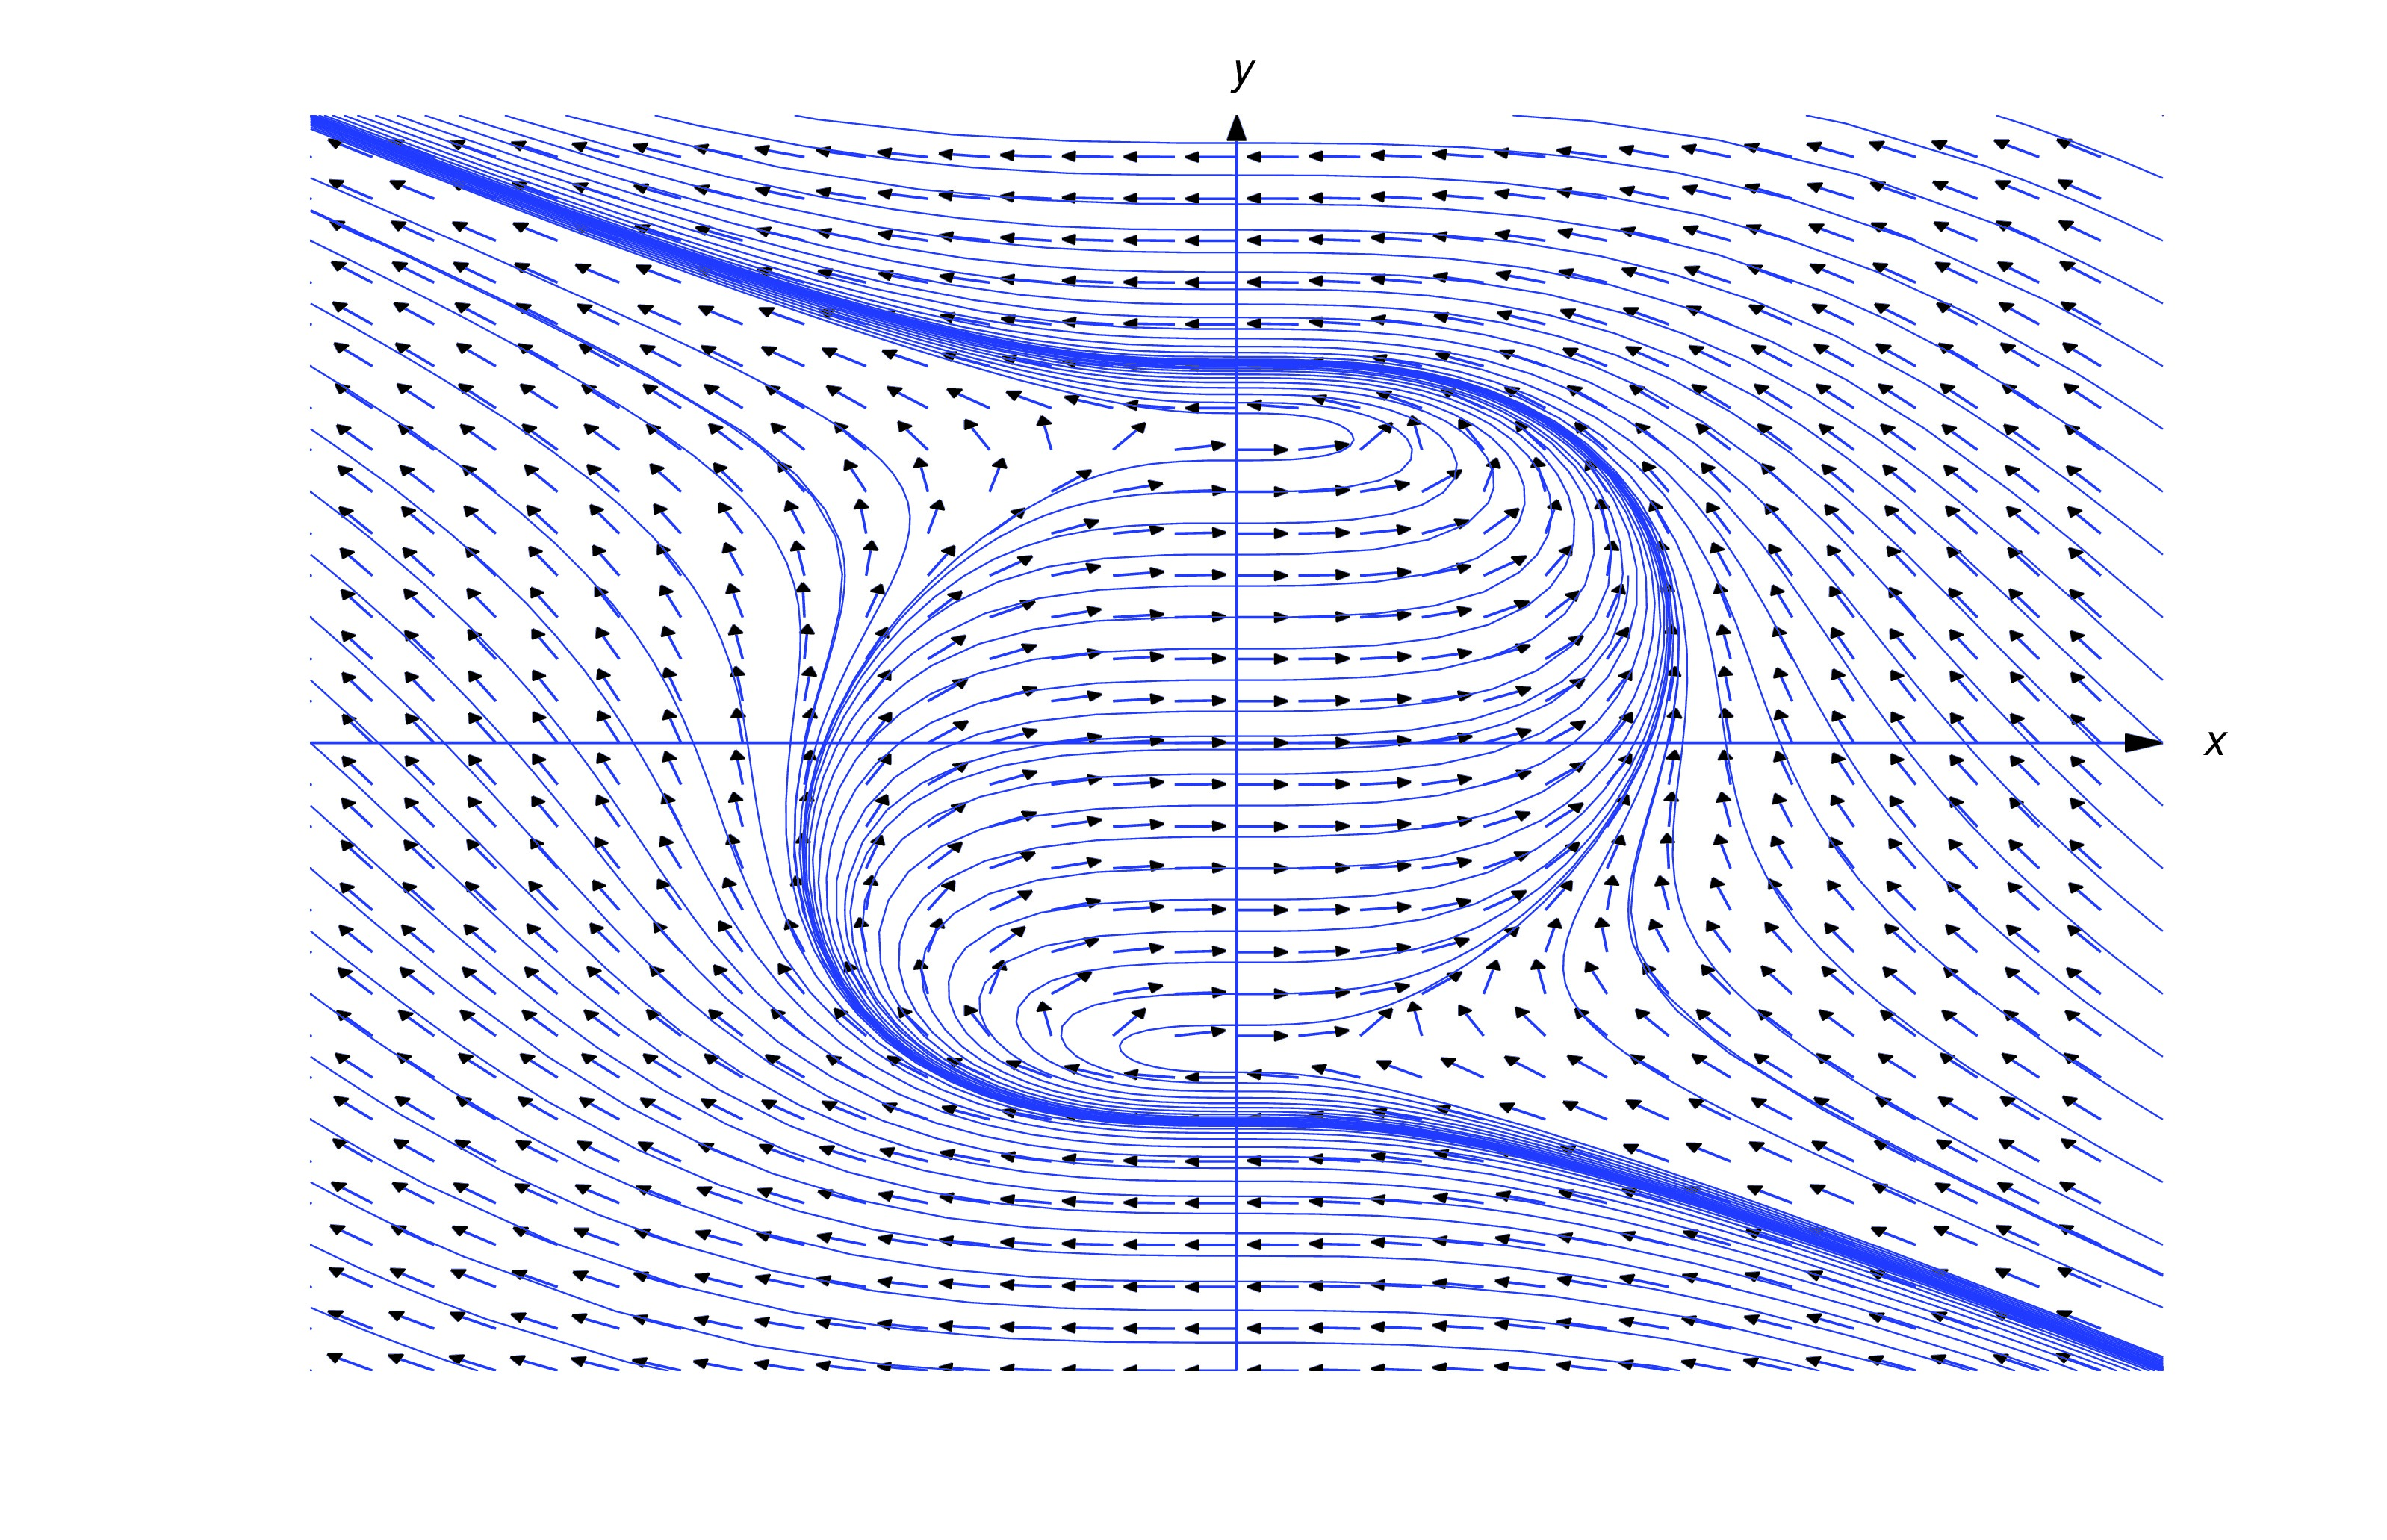
\includegraphics[scale=0.12]{figure/int_curve.jpeg}
    \caption{flow}
\end{figure}
Fix a smooth manifold $M$ and $V \in \frak{X}(M)$. For each $p \in M$, $V$ has a unique integral curve starting at $p$ and defined for all $t \in [0,\infty)$. Now let $p$ runs through all points of $M$, we get a map
\begin{align*}
    \cta: \R \times M &\to M \\
    (t,p) &\mapsto \cta(t,p). 
\end{align*}
Now we can take sections on $\R$ or $M$. 
\begin{itemize}
    \item Fix $p$, we get a map $\cta^{(p)}:\R \to M$ given by $\cta^{(p)}(t) = \cta(t,p)$, which is the point on the curve at time $t$ starting at $p$. This is essentially same as a parametrized curve. 
    \item Fix $t$, we get a map $\cta_t:M \to M$ given by $\cta_t(p) = \cta(t,p)$. This is to see how far can each integral curve travel in time $t$. 
    \begin{figure}[h]
        \centering
        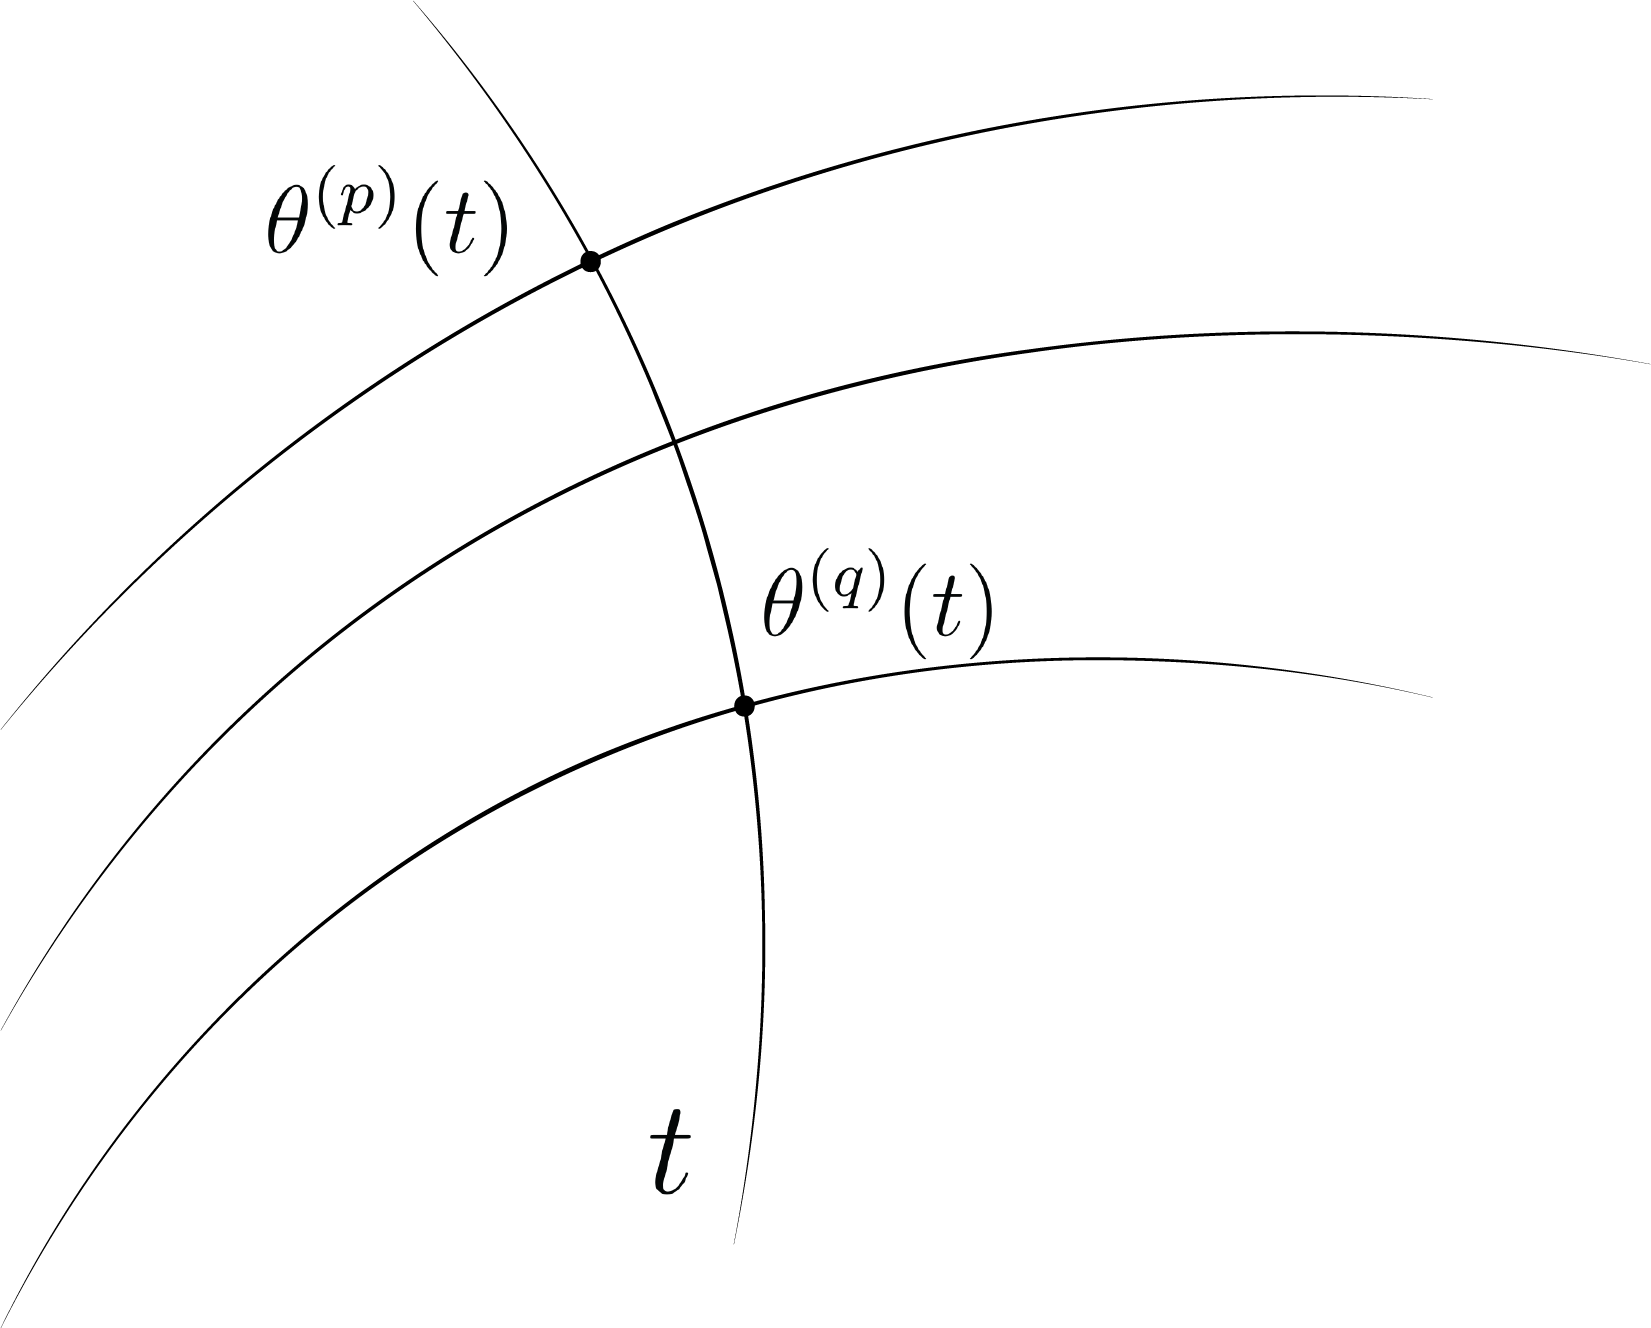
\includegraphics[scale=0.6]{figure/flow.png}
        \caption{Fix $t$, the position $\cta^{(p)}(t)$ and $\cta^{(q)}(t)$}
    \end{figure}
\end{itemize}

Suppose a curve $\cta^{(p)}$ is chosen and let $q$ be another point in this curve: $q = \cta^{(p)}(s)$ for some $s \in (0,\infty)$. By concatenating the time interval $[0, s]$, we can reparametrize $q$ w.r.t. $p$: 
$$\cta^{(q)}(t) = \cta^{(p)}(t+s), \quad t \in [0,\infty). $$
Now $\cta^{(q)}(0) = \cta^{(p)}(s) = q$ is the initial point of $\cta^{(q)}$. In fact, $\cta$ is an action of the group $(\R,+)$ on $M$. To see this, notice that 
\begin{itemize}
    \item $\cta_t \circ \cta_s(p) = \cta_t(\cta_s(p)) = \cta_t(q) = \cta^{(q)}(t) = \cta^{(p)}(t+s) = \cta_{t+s}(p)$.
    \item $\cta_0(p) = \cta^{(p)}(0) = p$. 
\end{itemize}
If we denote the the action by $t \cdot p = \cta^{(p)}(t)$, then 
$0 \cdot p = \cta^{(p)}(0) = p$, and 
$$t \cdot (s \cdot p) = t \cdot (\cta^{(p)}(s)) = t \cdot q = \cta^{(q)}(t) = \cta^{(p)}(t+s) = (t+s) \cdot p. $$
\begin{definition}[global flow]
A \textit{global flow} is a smooth map $\cta:\R \times M \to M$ such that 
\begin{itemize}
    \item $\cta(0,\cdot) = \id_M$,
    \item $\cta(t+s,p) = \cta(t,\cta(s,p))$ for all $s,t \in \R$ and $p \in M$. 
\end{itemize}
\end{definition}
Note that if $\cta_t = \cta(t,\cdot):M \to M$, then the map 
$$t \in (\R,+) \mapsto \cta_t \in \mathrm{Diff}(M)$$ is a homomorphism, since the second property implies that 
$$\cta_{t+s} = \cta_t \circ \cta_s, $$
and $\cta_t^{-1} = \cta_{-t}$ because $\cta_0 = \id_M$.

\begin{center}
    \line(1,0){400} \\[7pt]
    {\Large \textsc{Flow $\to $ Vector Field}} 
    \line(1,0){300} \\[3pt]
\end{center}
It is intuitive that if we take derivative at each point of each integral curve, we will obtain a vector field. 
\begin{definition}
    If $\cta: \R \times M \to M$ is a smooth global flow, for each $p \in M$ we define a tangent vector $V_p \in T_pM$ by 
    $$V_p = {\cta^{(p)}} '(0). $$
    The assignment $p \mapsto V_p$ is a vector field on $M$, which is called the \textit{infinitesimal generator} of $\cta$. 
\end{definition}
\begin{proposition}
    Let $\cta:\R \times M \to M$ be a global flow. Then 
    $$V_p = \dv{}{t}\bigg|_{t=0} \cta(t,p) \in T_pM $$ defines a smooth vector field on $M$. Moreover, each curve $\cta^{(p)}$ is an integral curve of $V$. 
\end{proposition}
\begin{proof}
    Rewrite the expression
    $$V_p = d\cta_{(0,p)}\br{\dv{}{t}\bigg|_{t=0}}, $$
    so $V$ is smooth (in local cooridnates $d\cta_{(0,p)}$ is a matrix whose entries depend smoothly on $p$), hence $V \in \frak{X}(M)$. For the moreover part, fix $p \in M$ and let $\ga(t) = \cta(t,p)$. Then 
    $$\ga'(t) = \dv{}{s}\bigg|_{s=0}\ga(t+s)
    = \dv{}{s}\bigg|_{s=0} \cta(t+s,p) 
    = \dv{}{s}\bigg|_{s=0} \cta(s, \cta(t,p)) 
    = V_{\cta(t,p)} = V_{\ga(t)}. $$
\end{proof}

\begin{center}
    \line(1,0){400} \\[7pt]
    {\Large \textsc{Vector Field $\to $ Flow}} 
    \line(1,0){300} \\[3pt]
\end{center}

Conversely, we would like to be able to say that every smooth vector field is the infinitesimal generator of a smooth global flow, which is not always the case. 
\begin{example}
    Let $M = \R^2 \setminus \{0\}$ and $V$ be the vector field $\pdv*{}{x}$ on $M$. The unique integral curve of $V$ starting at $(-1,0) \in M$ is $\ga(t) = (t-1, 0)$. In this case, $\ga$ cannot be extended continuously past $t=1$. Suppose this were true, let $\widetilde{\ga}$ be any continuous extension of $\ga$ past $t=1$, and notice that $\widetilde{\ga}$ is still a curve in $M = \R^2 \setminus \{0\}$.  
    Then $$\lim_{t \to 1^-}\ga(t) = \widetilde{\ga}(1) \in \R^2 \setminus \{0\}, $$ 
    but if we consider $\ga:M \to \R^2$, then 
    $$ \lim_{t \to 1^-}\ga(t) = \lim_{t \to 1^-} (t-1, 0) = (0,0) \neq \widetilde{\ga}(1), $$ a contradiction. \qed 
\end{example}

It seems that the domain is too large, so we have to restrict integral curves into a \textit{flow domain}.
\begin{definition}[flow domain]
    A \textit{flow domain} $\calD \subset \R \times M$ is an open set such that  for each $p \in M$, the section $\calD^{(p)} := \{t \in \R: (t,p) \in \calD\}$ is an open interval containing $0$. 
    A \textit{(partial) flow} is a smooth map $\cta:\calD \to M$ defined on a flow domain such that $\cta(0,\cdot) = \id_M$ and $\cta(t+s,p) = \cta(t, \cta(s,p))$ whenever both sides are defined. 
\end{definition}

\begin{example}
    Let $\D$ be the open disc in $\R^2$, let $V = \pdv*{}{x}$.
    
    integral curves don't exist for all time.
    Get a flow $\cta:D \to \D$ where $D \neq \R \times \D$.
\end{example}

\begin{definition}
    A \textit{maximal integral curve} is one that cannot be extended to an integral curve on any larger open interval, and a \textit{maximal flow} is a flow that admits no extension to a flow on a larger flow domain (i.e., a flow defined on a maximal flow domain)
\end{definition}

\begin{theorem}[fundamental theorem on Flows]\label{9.12}
    Let $V \in \frak{X}(M)$, there is a unique maximal flow $\cta:\calD \to M$ where $\displaystyle{V_p = \dv{}{t}\bigg|_{t=0} \cta(t,p)}$ for all $p \in M$. Moreover, 
    \begin{enumerate}
    \item for each $p \in M$, 
    $t \in \calD^{(p)} \mapsto \cta(t,p) \in M$ is the unique maximal integral curve starting at $p$.
    \item If $s \in \calD^{(p)}$, then $\calD^{(\cta(s,p))} = \calD^{(p)} \setminus \{s\}$.
    \end{enumerate}
\end{theorem}
\begin{proof}
    Use the existence theorem of an ODE to construct the slice $\calD^{(p)}$, and define a flow domain $\calD$.  
\end{proof}

\begin{definition}
    The flow in \textbf{Theorem \ref{9.12}} is called the \textit{flow generated by} $V$, or just the \textit{flow of} $V$. 
\end{definition}

\section{Complete Vector Fields}
A vector field is \textit{complete} if its flow is a global flow (i.e., defined on $\calD = \R \times M$, so that $\calD^{(p)} = \R$). 
\begin{lemma}[uniform time lemma]\label{9.15} %9.15
    Let $V \in \frak{X}(M)$ and $\cta:\calD \to M$ be the flow of $V$. If there exists $\eps>0$ such that $(-\eps, \eps) \subset \calD^{(p)}$ for all $p \in M$, then $V$ is complete. 
\end{lemma}
\begin{proof}
    Suppose to the contrary that for some $p \in M$, the domain $\calD^{(p)}$ is bounded above. Let $b = \sup \calD^{(p)}$, let $t_0>0$ be such that $b-\eps < t_0 < b$, and let $q = \cta^{p}(t_0)$. The hypothesis implies that $\cta^{(q)}(t)$ is defined at least for $t \in (-\eps, \eps)$. Concatenate $\cta^{(p)}$ and $\cta^{(q)}$ by a curve $\ga:(-\eps, \eps+t_0)$ defined as 
    $$ \ga(t) = \begin{cases}
        \cta^{(p)}(t), & \eps<t<b, \\
        \cta^{(q)}(t-t_0), & t_0-\eps < t < t_0+\eps. \end{cases}$$
    Since by the group law we have 
    $$\cta^{(q)}(t-t_0) = \cta_{t-t_0}(q) = \cta_{t-t_0}\circ \cta_{t_0}(p) = \cta_t(p) = \cta^{(p)}(t), $$
    these two definitions agree where they overlap. By the transition lemma, $\ga$ is an integral curve starting at $p$. Since $t_0+\eps \notin \calD^{(p)}$, this contradicts the maximality of the flow domain.  

    %Fix $p \in M$, then $D^{(p)} = (a,b)$ where $a \in \{-\infty\} \cup (-\infty, 0)$ and $b \in (0,\infty) \cup \{\infty\}$. Suppose for a contradiction that $b \neq \infty$, then $$(-\eps, \eps) \subset D^{(\cta(b-\eps/2, p))} = D^{(p)} \setminus \{b - \eps/2 \} \subset (-\infty, \eps/2), $$
\end{proof}
\begin{corollary} %9.17
    On a compact manifold, every vector field is complete. 
\end{corollary}
\begin{proof}
    See HW 8, Problem 1(a).    
\end{proof}

\begin{lemma}
    Suppose $M$ is a smooth manifold, $V \in \mathfrak{X}(M)$, and let $\theta: \mathcal{D} \rightarrow M$ be the flow of $V$. Then for any compact set $K \subset M$, there exists $\epsilon>0$ such that $(-\epsilon, \epsilon) \times K \subset \mathcal{D}$. 
\end{lemma}
\begin{proof}
    Since $\cta$ is a flow, $\calD$ is a flow domain. Thus for any $p \in M$, $$\calD^{(p)} = \{t \in \R: (t,p) \in \calD\} = (a_p, b_p) \ni 0.$$
    We also have $(a_p, b_p) \times \{p\} \subset \calD$, but $\calD$ is open in $\R \times M$, thus there exists an open set $U_p \ni p$ such that $(a_p, b_p) \times U_p \subset \calD$. For the cover $\{U_p\}_{p \in K}$ we can extract a finite subcover $\bCup{j=1}{n}U_{p_j} \supset K$, and each $U_{p_j}$ corresponds to a 
    $$\calD^{(p_j)} = \{t \in \R: (t,p_j) \in \calD \} = (a_{p_j}, b_{p_j}) \ni 0 $$ and 
    $(a_{p_j}, b_{p_j}) \times U_{p_j} \subset \calD$. Choose $0 < \eps < \min_{1\leq j \leq n} (|a_{p_j}|, |b_{p_j}|)$, we have $(-\eps, \eps) \subset (a_{p_j}, b_{p_j})$ for $j=1, \cdots, n$. Hence 
    $$(-\eps, \eps) \times U_{p_j} \subset \calD \quad \text{ for each } j=1, \cdots, n. $$
    Therefore, 
    $$(-\eps, \eps) \times K \subset (-\eps, \eps) \times \bCup{j=1}{n}U_{p_j} \subset \calD. $$
\end{proof}
\begin{lemma}[escape lemma]\label{9.19}
    If $\ga:J \to M$ is a maximal integral curve of $V$ whose domain $J$ has a finite least upper bound $b$, then for any $t_0 \in J$, $\ga([t_0,b))$ is not contained in any compact subset of $M$. 
\end{lemma}
\begin{proof}
    We may assume that $J = (a,b) \ni 0$. Suppose that there exists $t_0 \in J$ such that $\ga([t_0, b))$ is contained in a compact set $K$ of $M$. Set $p = \ga(a)$, then by the fundamental theorem of flow, there is a maxiaml flow $\cta:\calD \to M$. By uniquenss, $\cta^{(p)}:\calD^{(p)} \to M$ is exactly $\ga$ and $\calD^{(p)} = J$. Let $\{t_n\}_{n=1}^\infty \subset [t_0, b)$ converge to $b$, then $\{\ga(t_n)\}_{n=1}^\infty \subset K$. Then there is a subsequence $\{\ga(t_{n_k})\}_{k=1}^\infty$ with $\ga(t_{n_k})$ converging to some $q \in K$ as $k \to \infty$. By the last lemma, there exists $\eps>0$ such that $(-\eps, \eps) \subset [t_0, b)$ and 
    $(-\eps, \eps) \times K \subset \calD$, so $\cta$ is defined on $(-\eps, \eps) \times K$. Choose $n$ large so that $t_n > b - \eps$, and define $\b:(a, t_n + \eps) \to M$ by 
    $$\b(t) = \begin{cases}
        \ga(t), & a<t<b. \\
        \cta_{t-t_n} \circ \cta_{t_n}(p), & t_n-\eps < t < t_n + \eps.
    \end{cases}$$
    These two definitions agree where they overlap since
    $$\cta_{t-t_n} \circ \cta_{t_n}(p) = \cta_t(p) = \ga(t), $$
    hence $\b$ extends $\ga$ past $b$, a contradiction. 
\end{proof}




\section{Regular Points and Singular Points}
If $V \in \frak{X}(M)$, then $p \in M$ is a \textit{regular point} of $V$ if $V_p \neq 0$. Otherwise, if $V_p=0$, then $p$ is a \textit{singular point} of $V$. 
\begin{theorem}[canonical form near a regular point]\label{9.22}
    If $V \in \frak{X}(M)$, $p \in M$, and $V_p \neq 0$, then there exists a chart $(U,\phe=(x^1,\cdots,x^n))$ centered at $p$ where $V = \pdv*{}{x^i}$ on $U$. 
\end{theorem}
\begin{proof}
    
\end{proof}
\begin{remark}
    No canonical form near singular points: see Lee Figure 9.8.
\end{remark}
\section{Lie Derivatives}
\begin{definition}
    Suppose $V \in \frak{X}(M)$ has flow $\cta$. Then the \textit{Lie derivative} of $W \in \frak{X}(M)$ w.r.t. $V$ is the vector field where 
    $$\calL_V(W) = \dv{}{t}\bigg|_{t=0}d(\cta_{-t})_{\cta_t(p)}(W_{\cta_t(p)})
    = \lim_{t \to 0} \frac{d(\cta_{-t})_{\cta_t(p)}(W_{\cta_t(p)}) - W_p}{t}$$
\end{definition}
\begin{remark}
    $d(\cta_{-t})_{\cta_t(p)}(W_{\cta_t(p)}) \in T_{\cta_{-t}(\cta_t(p))} M$
\end{remark}
\begin{theorem}
    If $V,W \in \frak{X}(M)$, then $\calL_V(W) = [V,W]$. 
\end{theorem}
\begin{proof}
    Fix a chart $(U,\phe)$. In these coordinates 
    $$\cta(t,p) = (\cta^1(t,p), \cdots, \cta^n(t,p)), \quad 
    W = W^j \pdv{}{x^j}. $$
    \begin{align*}
    \calL_V(W) &= \dv{}{t}\bigg|_{t=0} {\pdv{\cta^i}{x^j}}(-t, \cta(t,x)) W^j(\cta(t,x)) \pdv{}{x^i} \\[10pt]
    &= -{\pdv[2]{\cta^i}{t}{x^j}} (-t, \cta(t,x))W^j(\cta(t,x))\pdv{}{x^i} + \pdv[2]{\cta^i}{x^k}{x^j}(-t, \cta(t,x)) {\pdv{\cta^k}{t}}(t,x) W^j(\cta(t,x)) \pdv{}{x^i} \\
    &\quad+ {\pdv{\cta^u}{x^j}} (-t, \cta(t,x)) {\pdv{W^j}{x^k}} (\cta(t,x)) {\pdv{\cta^k}{t}} (t,x) \pdv{}{x^i} \bigg|_{t=0} \\[10pt]
    &= {\pdv[2]{\cta}{t}{x^j}} (0,x) W^j(x) \pdv{}{x^i} + {\pdv[2]{\cta^i}{x^k}{x^j}} (0,x) {\pdv{\cta^k}{t}} (0,x) W^j(x) \pdv{}{x^i} \\
    &\quad+ {\pdv{\cta^i}{x^j}}(0,x) {\pdv{W^j}{x^k}}(x) {\pdv{\cta^k}{t}}(0,x). 
    \end{align*}
    Note 
    $${\pdv{\cta^k}{t}}(0,x) = V^k, \quad {\pdv[2]{\cta^i}{t}{x^j}}(0,x) =  \pdv{}{x^j} \br{{\pdv{\cta^i}{t}}(0,x)} = \pdv{V^i}{x^j}, $$
    and 
    $\cta(0,\cdot) = \id_M$, so 
    \begin{align*}
    &{\pdv{\cta^i}{x^j}}(0,x) = \begin{cases}
    1 & i = j, \\
    0 & i \neq j, \end{cases} \\
    &{\pdv[2]{\cta^i}{x^k}{x^j}} (0,x) = \pdv{}{x^k}\br{ {\pdv{\cta^i}{x^j}}(0,x) } = 0,
    \end{align*}
    then 
    \begin{align*}
    \calL_V(W) = -{\pdv{V^i}{x^j}}W^j\pdv{}{x^i} + 0 + \pdv{W^j}{x^k}V^k\pdv{}{x^j} = [V,W]. 
    \end{align*}
\end{proof}
\begin{corollary}\label{9.39}
    If $V,W,X,Y \in \frak{X}(M)$, then 
    \begin{enumerate}
    \item $\calL_V(W) = -\calL_W(V)$;
    \item $\calL_V([X,Y]) = [\calL_V X,Y] + [X,\calL_V Y]$;
    \item $\calL_{[V,W]}X = \calL_V \calL_W X - \calL_W \calL_V X$.
    \item If $g \in C^\infty(M)$, then 
    $$\calL_V(gW) = (Vg)W + g\calL_V(W).$$
    \item If $F:M \to N$ is a diffeomorphism, 
    $$F_*\calL_V(W) = \calL_{F_* V}(F_* W). $$
    \end{enumerate}
\end{corollary}
\begin{proof}
\begin{enumerate}
    \item $\calL_W(V) = [W,V] = -[V,W]$.
    \item $\calL_V([X,Y]) = [V,[X,Y]]$. Let $f \in C^\infty(M)$, then 
    \begin{align*}
    [V,[X,Y]]f &= V[X,Y]f - [X,Y]Vf \\
    &= V(XYf - YXf) - (XYVf-YXVf) \\
    &= VXYf - VYXf - XYVf + YXVf,
    \end{align*} and 
    \begin{align*}
    [\calL_V X,Y]f &= [[V,X],Y]f \\
    &= [V,X]Yf - Y[V,X]f \\
    &= VXYf - XVYf - YVXf + YXVf, \\
    [X,\calL_V Y]f &= [X,[V,Y]]f \\
    &= X[V,Y]f - [V,Y]Xf \\
    &= XVYf - XYVf - VYXf + YVXf.
    \end{align*}
    \item Similar as (2). 
    \item 
\end{enumerate}

\end{proof}
\section{Commuting Vector Fields}
\begin{definition}
\begin{itemize}
    \item We say that $V,W \in \frak{X}(M)$ are \textit{commute} if $[V,W] = 0$, i.e., $VWf = WVf$ for every smooth function $f$. 
    \item If $\cta:\calD \to M$ is a flow and $W \in \frak{X}(M)$, then $W$ is \textit{invariant} under $\cta$ if \begin{equation}
        d(\cta_t)_p W_p = W_{\cta_t(p)} \quad \text{for all }(t,p) \in \calD
    \end{equation}
    \item Two flows $\cta, \psi$ \textit{commute} if whenever $p \in M$ and $I,J \subset \R$ are open intervals containing $0$ such that one of $\psi_s \circ \cta_t(p)$ or $\cta_t \circ \psi_s(p)$ is defined for all $(s,t) \in I \times J$, then 
    $$\psi_s \circ \cta_t(p) = \cta_t \circ \psi_s(p) $$ for all $(s,t) \in I \times J$ (in particular both defined). 
\end{itemize}
\end{definition}

\begin{theorem} % 9.42 and 9.44
    If $V,W \in \frak{X}(M)$, then TFAE:
    \begin{enumerate}
    \item $V,W$ commute.
    \item $W$ is invariant under the flow of $V$. 
    \item $V$ is invariant under the flow of $W$.
    \item The flows of $V,W$ commute. 
    \end{enumerate}
\end{theorem}
\begin{proof}
    (a) $\iff$ (b). 

    (a) $\iff$ (c): Since $[V,W] = -[W,V]$, this follows from the equivalence of (a) and (b). 

    (b), (c) $\implies$ (d): By symmetry, it suffices to fix $p \in M$ and open intervals $I,J \subset \R$ containing $0$, where $\psi_s \circ \cta_t(p)$ exists for all $(s,t) \in I \times J$, then show that $\psi_s \circ \cta_t(p) = \cta_t \circ \psi_s(p)$ for all $(s,t) \in I \times J$. 
    Fix $s \in I$. Define $\ga:J \to M$ by $\ga(t) = \psi_s \circ \cta_t(p)$. Then $$\ga'(t) = d(\psi_s)_{\cta_t(p)} V_{\cta_t(p)} = V_{\psi_s(\cta_t(p))} = V_{\ga(t)}, $$
    so $\ga$ is an integral curve of $V$. Then $\ga(t) = \cta_t(\psi_s(p))$ for all $t \in J$ since $\ga(0) = \psi_s(p)$. Hence $\cta_t(\psi_s(p)) = \psi_s(\cta_t(p))$ for all $t \in J$. Since $s \in I$ was arbitrary, we are done.

    (d) $\implies$ (b): Fix $p \in M$, then $\psi_s \circ \cta(p) = \cta_t \circ \psi_s(p)$ for $s,t$ small enough. Then $$W_{\cta_t(p)} = \dv{}{s}\bigg|_{s=0}\psi_s(\cta_t(p)) = \dv{}{s}\bigg|_{s=0}\cta_t(\psi_s(p)) = d(\cta_t)_{p}W_p \quad (*) $$
    for $t$ small. To show this for any $t \in D^{(p)}$, use $(*)$ and the fact that 
    $$d(\cta_{t_1+t_2})_p = d(\cta_t)_{\cta_{t_2}(p)}d(\cta_{t_2})_p. $$
\end{proof}



\chapter{Vector Bundles}
    \section{Vector Bundles}
Goal: introduce the language of vector bundles. 
\begin{definition}
    Let $M$ be a topological space. A (real) vector bundle of rank $k$ over $M$ is a topological space $E$ and a surjective continuous map $\pi:E \to M$ such that
    \begin{itemize}
    \item for each $p \in M$, the fiber $E_p:=\pi^{-1}(p)$ is endowed with a $k$-dimensional real vector space structure.
    \item For each $p \in M$, there is a open neighborhood $U$ of $p$ and a homeomorphism
    $$ \Phi:\pi^{-1}(U) \to U \times \R^k $$
    (called the \textit{local trivialization} of $E$ over $U$) such that 
    \begin{itemize}
        \item $\pi_U \circ \Phi = \pi$ where $\pi_U:U \times \R^k \to U$ is the projection. 
        \item For each $q \in U$, the map $\Phi|_{E_q}: E_q \to \{q\} \times \R^k \simeq \R^k $ is a linear isomorphism.
    \end{itemize}
    \end{itemize}
    If $E,M$ are smooth manifolds, $\pi$ is smooth, and each $\Phi$ is a diffeomorphism, then $\pi:E \to M$ is a \textit{smooth vector bundle}.
\end{definition}

$E = $ total space of the vector bundle \\
$\pi =$ projection space of the vector bundle \\
$M = $ base space of the vector bundle 

\begin{example}
    $M \times \R^k \to M$ is the \textit{trivial bundle}. 
\end{example}
\begin{proof}
    Let $p \in M$, then $\pi^{-1}(p) = \{p\} \times \R^k \simeq \R^k$ is a $k$-dimensional vector space. Let $U$ be an open neighborhood of $p$, and define 
    \begin{align*}
        \Phi: \pi^{-1}(U) &\to U \times \R^k \\
        \Phi(p, x) &= (p, x). 
    \end{align*} Then $\Phi$ is clearly a homeomorphism. 
\end{proof}
\begin{example}
    Given a smooth manifold $M$, $TM \to M$ is a smooth vector bundle. 
\end{example}
\begin{proof}
    Suppose $\dim M = n$. Let $p \in M$, then $E_p := \pi^{-1}(p) = T_p M = \R^n$. Let $U$ be a neighborhood of $p$, then $\pi^{-1}(U)$ is the set of all tangent vectors at each point of $U$. Define
    \begin{align*}
        \Phi: \pi^{-1}(U) &\to U \times \R^n \\
        \Phi\br{v^i \dvBase{x^i}{p}} &= (p, v^1, \cdots, v^n),
    \end{align*}
    then $\Phi$ is a homeomorphism. Next,
    $$\pi_U \circ \Phi\br{v^i \dvBase{x^i}{p}} = \pi_U(p) = p, $$
    and $$\Phi|_{E_q}\br{v^i \dvBase{x^i}{q}} = (q, v^1, \cdots, v^n) $$ is clearly a linear isomorphism. 
\end{proof}
\begin{example}
    If $M \subset \R^n$ is an embedded submanifold, $NM \to M$ is a smooth vector bundle. 
\end{example}
\begin{example}
    Let $E = [0,1] \times \R / (0,t) \sim (1,-t)$, $\S^1 = [0,1] / 0 \sim -1$. Then $\pi:E \to \S^1$ defined by $\pi([x,t]) = [x]$ is a vector bundle. 
\end{example}

\section{Transition Functions}
\begin{lemma}\label{10.5}
    Let $\pi:E \to M$ be a smooth vector bundle of rank $k$. Suppose $$\Phi:\pi^{-1}(U) \to U \times \R^k, \quad \Psi: \pi^{-1}(V) \to V \times \R^k$$ are smooth local trivializations with 
    $U \cap V \neq \varnothing$. Then 
    $$\Phi \circ \Psi^{-1}(p, w) = (p, \tau(p)w)$$
    on $(U \cap V) \times \R^k$, where $\tau:U \cap V \to \mathrm{GL}(k,\R)$ is smooth. $\tau$ is called the \textit{transition function} between the  trivializations.
\end{lemma}
\begin{proof}
    By definition, $$\Phi \circ \Psi^{-1}(p,v) = (p, \tau(p)v)$$ for some map $\tau:U \cap V \to \mathrm{GL}(k,\R)$. To show that $\tau$ is smooth, it suffices to show that the $(i,j)$-entry $\tau(p)_j^i$ is smooth. Let $E_1, \cdots, E_k$ be the standard basis of $\R^k$. Let $\pi^i:\R^k \to \R$ be the projection onto the $i$th entry. Let $\widehat{\pi}:(U \cap V) \times \R^k \to \R^k$ be the projection. Then
    \begin{align*}
    \tau(p)_j^i &= \pi^i(\tau(p)E_j) 
    = \pi^i(\widehat{\pi}(\Phi \circ \Psi^{-1}(p, E_j)) 
    \end{align*}
    is smooth. 
\end{proof}
\begin{lemma}[vector bundle chart lemma]\label{10.6}
    Let $M$ be a smooth manifold. For each $p \in M$, suppose $E_p$ is a real vector space of dimension $k$. Let $E = \bigsqcup_{p \in M}E_p$ and let $\pi:E \to M$ be the map with $\pi_{E_p} = p$ for all $p \in M$. Suppose we are given:
    \begin{enumerate}
        \item an open cover $\{U_\a\}_{\a \in A}$ of $M$. 
        \item For each $\a \in A$, a bijection $\Phi_\a:\pi^{-1}(U_\a) \to U_\a \times \R^k$, where $\Phi_\a|_{E_p}:E_p \to \{p\} \times \R^k \simeq \R^k$ is a linear isomorphism for all $p \in U_\a$. 
        \item For each $\a, \b \in A$ with $U_\a \cap U_\b$ nonempty, there is a smooth map $\tau_{\a \b}:U_\a \cap U_\b \to \mathrm{GL}(k,\R)$ such that 
        $$\Phi_a \circ \Phi_\b^{-1}(p,v) = (p, \tau_{\a\b}(p)v)$$ on $(U_\a \cap U_\b) \times \R^k$. 
    \end{enumerate}
    Then $E$ has a unique topology and smooth structure making $\pi:E \to M$ a smooth vector bundle of rank $k$ where each $\Phi_\a$ is a local trivialization. 
\end{lemma}
\begin{proof}
    Topology: See Lee. \\
    Smooth Structure: Let 
    $$\calA = \bigcup_{\a \in A} \{(\widetilde{U}, \widetilde{\phe}): (U,\phe) \text{ a smooth chart of }M\text{ where }U \subset U_\a \}, $$
    where 
    $$\widetilde{U} = \pi^{-1}(U) = \bigcup_{p \in U}E_p, \quad \widetilde{\phe} = (\phe \times \id_{\R^k}) \circ \Phi_\a. $$ We claim that $\calA$ is a smooth atlas covers $M$, since $M = \bigcup_{\a \in A}U_\a$. If $(\widetilde{U}, \widetilde{\phe}), (\widetilde{W}, \widetilde{\psi}) \in \calA$, then 
    \begin{align*}
    \widetilde{\phe} \circ \widetilde{\psi}^{-1}(x,v)
    &= (\phe \times \id_{\R^k}) \circ \Phi_\a \circ \Phi_\b^{-1} \circ (\psi \times \id_{\R^k})^{-1}(x,v) \\
    &= (\phe \times \id_{\R^k}) \circ \Phi_\a \circ \Phi_\b^{-1}(\psi^{-1}(x), v) \\
    &= (\phe \times \id_{\R^k})(\psi^{-1}(x), \tau_{\a\b}(\psi^{-1}(x), v)) \\
    &= (\phe \circ \psi^{-1}(x), \tau_{\a\b}(\psi^{-1}(x), v)).
    \end{align*}
    is smooth, so $\calA$ is a smooth atlas. \\
    Vector Bundle: Check that $\Phi_\a$ are smooth local trivializations. 
\end{proof}
\begin{example}[(Whitney Sums)]
    Suppose $\pi_1: E_1 \to M, \pi_2: E_2 \to M$ are smooth vector bundles. Let $E_p = E_{1p} \oplus E_{2p}$ and $E = \bigsqcup_{p \in M}E_p$. Then the projection $\pi:E \to M$ is a smooth vector bundle (called the Whitney sum of $E_1$ and $E_2$). 
\end{example}
\begin{proof}
    Fix an open cover $M = \bigcup_{\a}U_\a$ such that there are smooth local trivializations $\Phi_{i\a}:\pi_i^{-1}(U_\a) \to U_\a \times \R^{k_i}$. Let $\tau_{i\a\b}:U_\a \cap U_\b \to \GL(k_i, \R)$ be the transition functions.
    Define $\Phi_\a:\pi^{-1}(U_\a) \to U_\a \times \R^{k_1+k_2}$ by 
    $$\Phi_\a((v_1,v_2)) = (\pi_1(v_1), (\pi_{\R^{k_1}}(\Phi_{i\a}(v_1)), \pi_{\R^{k_2}}(\Phi_{i\a}(v_2)) ) ).$$
    Note that $\pi_1(v_1) = \pi_2(v_2)$ since $(v_1,v_2) \in E_p = E_{1p} \oplus E_{2p}$. 
    Define $\tau_{\a\b}: U_\a \cap U_\b \to \GL(k_1+k_2, \R)$ by 
    $$\tau_{\a\b}(p) = \begin{pmatrix}
    \tau_{1\a\b}(p) & 0 \\
    0 & \tau_{2\a\b}(p) \end{pmatrix}. $$
    Check that this satisfies the lemma. 
\end{proof}
\begin{example}[(Dual)]
    Suppose $\pi:E \to M$ is a smooth vector bundle. Let $E_p^* = (E_p)^*$ be the dual of $E_p$. Let $E^* = \bigsqcup_{p \in M}E_p^*$, then the projection $\pi:E^* \to M$ is a smooth vector bundle (called the \textit{dual} to $E$). 
\end{example}
\begin{proof}
    Check on HW. 
\end{proof}

\section{Sections of Vector Bundles}\label{section of VB}
Let $\pi:E \to M$ be a vector bundle. A \textit{section} of $E$ is a continuous map $\sigma: M \to E$ such that $\pi \circ \sigma = \id_M$ (so that $\sigma$) is injective. 
\begin{example}
    Sections of $TM$ are vector fields on $M$. 
\end{example}
\begin{definition}
    If $f \in C^\infty(M)$ and $\sigma$ is a section of $E$, then define a new section $f \sigma$ by 
    $$(f\sigma)(p) = f(p)\sigma(p). $$
\end{definition}


\section{Maps Between Bundles}
\begin{definition}
    Suppose $\pi_1:E_1 \to M_1, \quad \pi_2:E_2 \to M_2$ are two vector bundles. A continuous map $F:E_1 \to E_2$ is a \textit{vector bundle homomorphism} if
    \begin{enumerate}
    \item there is a continuous map $f:M_1 \to M_2$ such that 
    \begin{center}
        \begin{tikzcd}
        E_1 \arrow[r, "F"] \arrow[d, "\pi_1"]& E_2 \arrow[d, "\pi_2"]   \\
        M_1 \arrow[r, "f"] & M_2 
        \end{tikzcd}
    \end{center}
    \item For each $p$, $F|_{E_{1p}}: E_{1p} \to E_{2f(p)}$ is linear.
    \end{enumerate}
    Moreover, 
    \begin{itemize}
    \item if $E,f$ are homeomorphisms, $F$ is a \textit{bundle isomorphism}.
    \item If everything is smooth, we add the word smooth to $F$.
    \end{itemize}
\end{definition}
\begin{remark}
    If $F$ is a bundle homomorphism, then $F$ is a bundle isomorphism if and only if $F$ is bijective and $F^{-1}$ is a bundle homomorphism. 
\end{remark}
\begin{example}
    If $F:M \to N$ is smooth, then $dF:TM \to TN$ is a smooth bundle homomorphism. 
\end{example}
    \section{Cotangent Bundles}
\subsection{Covector Fields}
For the rest of the chapter, fix a smooth manifold $M$.
Let $V$ be a finite-dimensional vector space, a \textit{covector} on $V$ is defined to be a real-valued linear functional on $V$. 
\begin{definition}
    For each $p \in M$, we define the \textit{cotangent space} at $p$ to be the dual space to $T_pM:$
    $$T_p^*M := (T_pM)^*. $$
    Elements of $T_p^*M$ are called \textit{tangent covectors} at $p$, or just covectors at $p$. 
\end{definition}
\begin{definition}
    Let $T^*M = \bigsqcup_{p \in M}T_p^*M$, then $T^*M$ is called the \textit{cotangent bundle} of $TM$.
\end{definition}
There is a natural projection $\pi:T^*M \to M$ given by $\omg \in T_p^*M \mapsto p \in M$. 

Fix a chart $(U,\phe)$ of $M$. If $p \in U$, let $dx^1|_p, \cdots, dx^n|_p \in T_p^*M$ be the dual basis to $\pdv*{}{x^1}|_p, \cdots, \pdv*{}{x^n}|_p \in T_pM$ so that 
$$ dx^i|_p\br{\pdv{}{x^j}\bigg|_p} = \begin{cases}
1 & i=j, \\
0 & i \neq j. \end{cases} $$
Next, let $\widetilde{U} = \pi^{-1}(U) \subset T^*M$ and define $\widetilde{\phe}:\widetilde{U} \to \R^n \times \R^n$ by 
$$\widetilde{\phe}\br{\xi_i dx^i|_p} = \br{\phe(p), \xi_1, \cdots, \xi_n}. $$
\begin{proposition}
    $(\widetilde{U}, \widetilde{\phe})$ is a smooth chart of $T^*M$. 
\end{proposition}
\begin{proof}
    Check. 
\end{proof}


A section $w:M \to T^*M$ is called a \textit{covector field}. Given a chart, we can write $w = w_i dx^i$ on $U$ where $w_1, \cdots, w_n:U \to \R$ are the component functions of $w$. 
\begin{proposition}\label{11.11}
    A covector field is smooth if and only if for every chart its component functions are smooth. 
\end{proposition}
\begin{proof}
    
\end{proof}
We let $\frak{X}^*(M)$ be the vector space of covector fields. 
\subsection{Differential of a Function}
Given $f \in C^\infty(M)$, if we identify $T_x\R = \R$ for all $x \in \R$, then $df_p \in T_p^*M$. Recall 
$$df_p(v) = v(f), $$ equivalently, 
$$df_p(v) = \dv{}{t}\bigg|_{t=0} (f \circ \ga)(t), $$ where $\ga:I \to M$ is a smooth curve with $\ga(0) = p, \ga'(0) = v$. 
\begin{remark}
    On a chart $(U,\phe)$, 
    \begin{itemize}
    \item $df = \pdv{f}{x^i} dx^i$, so $f$ is smooth. 
    \item $dx^i \in \frak{X}(U)$ is the differential of $x^i:U \to \R$, the $i$th component of $\phe$. 
    \end{itemize}
\end{remark}

\chapter{Tensors}
    \section{Multilinear Algebra}

\begin{definition}
Let $V_1, \cdots, V_k$ and $W$ be vector spaces. A map $F:V_1 \times \cdots \times V_k \to W$ is called \textbf{multilinear} if 
$$F(u_1, \cdots, au_i + bv_i, \cdots, u_k) = aF(u_1, \cdots, u_i, \cdots, u_k) + 
bF(u_1, \cdots, v_i, \cdots, u_k) \quad \text{for each }i. $$
\end{definition}
Denote $\calL(V_1, \cdots, V_k;W)$ for the set of all multilinear maps from $V_1 \times \cdots \times V_k$ to $W$. 
\begin{remark}
    We all know that $V_1 \times \cdots V_k$ is also a vector space, however, a multilinear map $F$ on this vector space is different from a linear map on this vector space. Take $k=2$, then 
    $$F(av_1, av_2) = aF(v_1, av_2) = a^2 F(v_1, v_2). $$
    As a product space, $a(v_1, v_2) = (av_1, av_2)$. 
\end{remark}
\begin{example}
    \begin{enumerate}
    \item The dot product in $\R^n$ is a bilinear function of two vectors. 
    $$\net{v,w} \in \R^n \times \R^n \mapsto v \cdot w \in \R$$ is in $\calL(\R^n, \R^n; \R)$.
    \item The cross product 
    $$(v,w) \in \R^3 \times \R^3 \mapsto v \times w \in \R^3 $$ is in $\calL(\R^3, \R^3; \R^3)$.
    \item The determinant is a real-valued multilinear function of $n$ vectors in $\R^n$. 
    \end{enumerate}
\end{example}
\begin{proof}
    Let $a \in \R$, then $\net{au+bv, w} = a\net{u, w} + b\net{v, w}$. Let $v_i \in \R^n$, then 
    $$\det [v_1 \cdots av_i+bv_j \cdots v_n ] = a\det[v_1 \cdots v_n] + b\det [v_1 \cdots v_n]. $$
\end{proof}
\begin{definition}
    Given $F \in \calL(V_1, \cdots, V_k; \R)$ and $G \in \calL(W_1, \cdots, W_l; \R)$, define the \textit{tensor (product)} of $F$ and $G$ by $F \otimes G \in \calL(V_1, \cdots, V_k, W_1, \cdots, W_l, \R)$ by 
    \begin{align*}
    F \otimes G(v_1, \cdots, v_k, w_1, \cdots, w_l) = F(v_1, \cdots, v_k)G(w_1, \cdots, w_l).
    \end{align*}
\end{definition}

\begin{example}
    Let $E_1, \cdots, E_n$ be the standard basis of $\R^n$ and $\eps^1, \cdots, \eps^n$ be the dual basis. Then 
    $$ v \cdot w = \br{\Sum{i=1}{n}\eps^i \otimes \eps^i}(v,w) $$ for all $v,w \in \R^n$. For each $i$, 
    $$\eps^i \otimes \eps^i(v_1, \cdots, v_n)\eps^i(w_1,\cdots,w_n) = v_i w_i. $$
\end{example}
\begin{example}
    ({\color{blue} Need to be justified}) 
    Let $(\Omg, \calF, \P)$ be a probability space, and let $X_1, \cdots, X_n$ be integrable independent variables, that is, $\E X_j < \infty$ for all $j$, where $\E$ is the expectation. Note that $\E$ is a linear map on $L^1(\Omg)$, and we write $\E \in \calL(L^1, \R)$. Then $\E(X_1)\E(X_2) = \E \otimes \E(X_1, X_2) = \E(X_1 X_2)$. 
\end{example}


\begin{proposition}\label{12.4}
    Let $V_1, \cdots, V_k$ be a vector space of dimension $n_1, \cdots, n_k$. For each $j = 1, \cdots, k$, let $E_1^{(j)}, \cdots E_{n_j}^{(j)}$ be a basis of $V_j$ and 
    $\eps_{(j)}^{1}, \cdots, \eps_{(j)}^{n_j}$ be the dual basis, then 
    $$\calB = \cBr{\eps_{(1)}^{i_1} \otimes \cdots \otimes \eps_{(k)}^{i_k}: 1\leq i_j \leq n_j \text{ for }j=1, \cdots, k}$$ is a basis for $\calL(V_1, \cdots, V_k; \R)$.
    $$\begin{array}{ccc}
    \text{vector space} & \text{basis} & \text{dual basis} \\
    V_1 & E_1^{(1)}, E_2^{(1)}, \cdots, E_{n_1}^{(1)} & \eps_{(1)}^{1}, \cdots, \eps_{(1)}^{n_1}\\
    V_2 & E_1^{(2)}, E_2^{(2)}, \cdots, E_{n_2}^{(2)} & \eps_{(2)}^{1}, \cdots, \eps_{(2)}^{n_2}\\
    \vdots & \\
    V_k & E_1^{(k)}, E_2^{(k)}, \cdots, E_{n_k}^{(k)} & \eps_{(k)}^{1}, \cdots, \eps_{(k)}^{n_k}
    \end{array}$$
\end{proposition}
\begin{proof}
    Fix a multi-linear function $F \in \calL(V_1, \cdots, V_k; \R)$. 
    Define coefficients 
    $$F_{i_1, \cdots, i_k} = F\br{E_{i_1}^{(1)}, \cdots, E_{i_k}^{(k)} }, $$ then (using Einstein summation)
    \begin{align*}
    F(v_1, \cdots, v_k) &= F
    \br{ v_1^{i_1}E_{i_1}^{(1)}, \cdots, v_k^{i_k}E_{i_k}^{(k)} } \\
    &= v_1^{i_1} \cdots v_k^{i_k}F
    \br{ E_{i_1}^{(1)}, \cdots, E_{i_k}^{(k)} } \\
    &= v_1^{i_1} \cdots v_k^{i_k} F_{i_1, \cdots, i_k} \\
    &= \br{F_{i_1, \cdots, i_k} \eps_{(1)}^{i_1} \otimes \cdots \otimes \eps_{(k)}^{i_k} } (v_1, \cdots, v_k). 
    \end{align*}
    If we do not use Einstein summation, the above sum can be written as 
    \begin{align*}
    &F\br{
    \sum_{i_1}v_1^{i_1}E_{i_1}^{(1)}, \sum_{i_2}v_2^{i_2}E_{i_2}^{(2)}, \cdots,
    \sum_{i_k}v_k^{i_k}E_{i_k}^{(k)}
    } \\
    &= \sum_{i_1}v_1^{i_1}F\br{
    E_{i_1}^{(1)}, \sum_{i_2}v_2^{i_2}E_{i_2}^{(2)}, \cdots, \sum_{i_k}v_k^{i_k}E_{i_k}^{(k)}
    } \\
    &= \sum_{i_1}v_1^{i_1} \sum_{i_2}v_2^{i_2} F\br{
    E_{i_1}^{(1)}, E_{i_2}^{(2)}, \cdots, \sum_{i_k}v_k^{i_k}E_{i_k}^{(k)}
    } = \cdots \\
    &= \sum_{i_1}v_1^{i_1} \sum_{i_2}v_2^{i_2} \cdots \sum_{i_k}v_k^{i_k} 
       F\br{ E_{i_1}^{(1)}, \cdots, E_{i_k}^{(k)} } \\
    &= \sum_{i_1,\cdots,i_k} v_1^{i_1} \cdots v_k^{i_k}
       F\br{ E_{i_1}^{(1)}, \cdots, E_{i_k}^{(k)} } \\
    &= \sum_{i_1,\cdots,i_k} v_1^{i_1} \cdots v_k^{i_k}F_{i_1,\cdots,i_k}.     
    \end{align*}
    Recall the definition of a dual basis, we have
    $$v_1^{i_1} = \eps_{(1)}^{i_1}\br{
    \Sum{j=1}{n_1} v_1^j E_{j}^{(1)}
    } = \eps_{(1)}^{i_1}(v_1). $$
    Then
    \begin{align*}
    \sum_{i_1,\cdots,i_k} v_1^{i_1} \cdots v_k^{i_k}F_{i_1,\cdots,i_k}
    &= \sum_{i_1,\cdots,i_k} \eps_{(1)}^{i_1}(v_1) \cdots \eps_{(k)}^{i_k}(v_k)
       F_{i_1,\cdots,i_k} \\
    &= \sum_{i_1,\cdots,i_k} F_{i_1,\cdots,i_k}
       \left[\eps_{(1)}^{i_1} \cdOtimes \eps_{(k)}^{i_k} (v_1,\cdots,v_k)\right].
    \end{align*}

    
    Now we show $\calB$ is linearly independent.
    Suppose $\a_{i_1, \cdots, i_k} \eps_{(1)}^{i_1} \otimes \cdots \otimes \eps_{(k)}^{i_k} = 0$, then
    \begin{align*}
    0 = \br{\a_{i_1, \cdots, i_k} \eps_{(1)}^{i_1} \otimes \cdots \otimes \eps_{(k)}^{i_k}}\br{E_{j_1}^{(1)}, \cdots, E_{j_k}^{(k)}}
    = \a_{j_1, \cdots, j_k}
    \end{align*}
    for all indices $j_1, \cdots, j_k$.
\end{proof}
    \section{Abstract Tensor Products}
\subsection{Free Vector Spaces}
Given a set $S$, 
\begin{itemize}
    \item A \textit{formal linear combination} of elements in $S$ is a function $f:S \to \R$, where $$\#\{x \in S: f(x) \neq 0\} < \infty.$$
    In this case we write $f = \Sum{i=1}{m}c_i x_i$, where $\{x_1, \cdots, x_m\} = \{x \in S: f(x) \neq 0\}$, and $c_i = f(x_i)$. 
    \item The \textit{free vector space} of $S$ denoted by $\calF(S)$ is the vector space of formal linear combinations. We view $S$ as a subset of $\calF(S)$ by identifying $x \in S$ with $\d_x \in \calF(S)$, where $\d_x(y) = \begin{cases} 1, & x = y \\ 0, & x \neq y \end{cases},$ so $f = \Sum{i=1}{m}c_i x_i = \Sum{i=1}{m}c_i \d_{x_i}$.
\end{itemize}
Rigorously, $\calF(S)$ is the vector space of functions $f \in \R^S$, but in practice we think of $S$ as a subset of $\calF(S)$ ($S$ is just a set). Typically we identify $x \in S$ with $\delta_x \in \R^S$. 

{\color{blue}There are many formal linear combinations. Is it possible to construct 
a sequence of formal linear combinations $\#\{x \in S: f_n(x) \neq 0\} = n$? }
\begin{example}
    Let $S = \{1, 2\}$, then $\#\{x \in S: f_n(x) \neq 0\} \leq 2$, and thus all functions from $S$ to $\R$ is a formal linear combination. Thus $\calF(S) = \R^S$. 
\end{example}
\begin{example}
    Let $S = \R$ and $f$ be a formal linear combination, then $\supp f = \{x_1, \cdots, x_m\}$, so we can write $f = \Sum{i=1}{m}c_i \d_{x_i}$. In this case $\Im f = \{c_1, \cdots, c_m\}$. Hence 
    $$\calF(\R) = \cBr{
    f \in \R^S: f = \Sum{i=1}{m}c_i \d_{x_i}, m \in \N, x_i \in \R \text{ distinct}
    },$$ which is a vector subspace of $\R^S$ (think of simple functions in real analysis, but assume values on a finite set).
\end{example}
\begin{example}
    Let $S = \R^d$, then 
    $$\calF(\R^d) = \cBr{
    f \in (\R^d)^S: f = \Sum{i=1}{m}c_i \d_{x_i}, m \in \N, x_i \in \R^d \text{ distinct}
    },$$
\end{example}
\begin{example}
    Let $V_1, V_2$ be finite-dimensional vector spaces, then 
    $$\calF(V_1 \times V_2) = \cBr{
    f \in (V_1 \times V_2)^S: f = \Sum{i=1}{m}c_i \d_{(v_1,v_2)}, m \in \N, v_i \in V_i
    },$$
\end{example}


\begin{proposition}\label{12.5}
    If $W$ is a vector space, then every map $A:S \to W$ has a unique extension to a linear map
    $\cl{A}:\calF(S) \to W$. 
\end{proposition}
\begin{proof}
    Check that 
    $$\cl{A}\br{\Sum{i=1}{m}c_i x_i} = \Sum{i=1}{m}c_i A(x_i) $$ defines $\cl{A}$. 
    Let $\Sum{i=1}{m}c_i x_i, \Sum{i=1}{m}d_i y_i \in \calF(S)$, then 
    \begin{align*}
    \cl{A}\br{\Sum{i=1}{m}c_i x_i + \Sum{i=1}{m}d_i y_i} 
    &= \cl{A}\br{\Sum{i=1}{m}(c_i x_i + d_i y_i)} \\
    &= \Sum{i=1}{m} \cl{A}(c_ix_i + d_iy_i) \\
    &= \Sum{i=1}{m} c_iA(x_i) + d_iA(y_i) \\
    &= \cl{A}\br{\Sum{i=1}{m}c_i x_i} + \cl{A}\br{\Sum{i=1}{m}d_i y_i}.
    \end{align*}
    Let $\lam \in \R$, then 
    $$\cl{A}\br{\lam \Sum{i=1}{m}c_i x_i} = \cl{A}\br{\Sum{i=1}{m} \lam c_i x_i}
    = \Sum{i=1}{m}\lam c_i A(x_i) = \lam \cl{A}\br{\Sum{i=1}{m}c_i x_i}. $$
\end{proof}

\subsection{Tensor Products}
Given $V_1, \cdots, V_k$ vector spaces, Let $\calR \subset \calF(V_1 \times \cdots \times V_k)$ be the linear subspace spanned by elements of the form 
    \begin{align*}
    (w_1, \cdots, w_{i-1}, aw_i, w_{i+1}, \cdots, w_k) - a(w_1, \cdots, w_k)
    \end{align*} and 
    \begin{align*}
    &(w_1, \cdots, w_{i-1}, w_i + w_i', w_{i+1}, \cdots, w_k) \\
    &- (w_1, \cdots, w_i, \cdots, w_k) - (w_1, \cdots, w_{i-1}, w_i', w_{i+1}, \cdots, w_k).  
    \end{align*}
Then
\begin{itemize} 
    \item The \textit{tensor product} of $V_1, \cdots, V_k$ is the vector space 
    $$V_1 \otimes \cdots \otimes V_k = \calF(V_1 \times \cdots \times V_k) / \calR. $$
    \item Let $\Pi:\calF(V_1 \times \cdots \times V_k) \to V_1 \otimes \cdots \otimes V_k$ be the projection and define the \textit{tensor product} of $w_1, \cdots, w_k$ as
    $$w_1 \otimes \cdots \otimes w_k = \Pi(w_1, \cdots, w_k)$$ where $w_i \in V_i$. This is the equivalence class of $(v_1, \cdots, v_k)$ in $V_1 \cdOtimes V_k$. 
\end{itemize}
\begin{remark}
    By definition, 
    \begin{align*}
    a \cdot (w_1 \otimes \cdots \otimes w_k) 
    &= (aw_1) \otimes w_2 \otimes \cdots \otimes w_k \\
    &= w_1 \otimes (aw_2) \otimes w_3 \otimes \cdots \otimes w_k
    &= w_1 \otimes \cdots \otimes w_{k-1} \otimes (aw_k)
    \end{align*} and 
    \begin{align*}
    &w_1 \otimes \cdots \otimes w_{i-1} \otimes (w_i + w_i') \otimes w_{i+1} \otimes \cdots \otimes w_k \\
    &= w_1 \otimes \cdots \otimes w_k + w_1 \otimes \cdots \otimes w_{i-1} \otimes w_i' \otimes w_{i+1} \otimes \cdots \otimes w_k
    \end{align*}
    for all $w_j \in V_j, w_j' \in V_j, a \in \R, i=1,\cdots, k$.
\end{remark}

We review a property of quotient vector space.
\begin{lemma}
    Let $W$ be a vector space and $V$ be a subspace of $W$, let $T:W \to X$ be a linear map. Then $T$ descends\footnote{Think of as ``$T$ induces a map $\widetilde{T}$''. } 
    to $\widetilde{T}:W / V \to X$ iff $V \subset \ker T$, where $\widetilde{T}(w+V) = Tw$. 
\end{lemma}
\begin{proof}
    Suppose $V \subset \ker T$. If $u+V = w+V$, then $u-w \in V \subset \ker T$, so $T(u-w) = Tu - Tw = 0$. Hence $\widetilde{T}(u+V) = \widetilde{T}(w+V)$, so $\widetilde{T}$ is well-defined, and it is clearly linear. 

    Conversely, suppose $T$ descends to a linear map $\widetilde{T}:W/V \to X$. Then $\widetilde{T}(u+V) = Tu = 0$ for all $u \in V$, hence $V \subset \ker T$.  
\end{proof}

\begin{proposition}[Characteristic Property]\label{12.7}
    If $A \in \calL(V_1, \cdots, V_k; W)$, then there is a unique linear map $\widetilde{A}:V_1 \otimes \cdots \otimes V_k \to W$ such that the following diagram commutes:
    \begin{center}
        \begin{tikzcd}
        V_1 \times \cdots \times V_k \arrow[r, "A"] \arrow[d, "\pi"]& W \\ 
        V_1 \otimes \cdots \otimes V_k
        \arrow[ur, "\widetilde{A}", labels=below right]
        \end{tikzcd}
    \end{center}
    where $\pi(v_1,\cdots,v_k) = v_1 \otimes \cdots \otimes v_k$. 
\end{proposition}
\begin{proof}
    First extend $A$ to $\cl{A}: \calF(V_1 \times \cdots \times V_k) \to W$, then 
    $$\cl{A}\br{\Sum{i=1}{m}c_i x_i} = \Sum{i=1}{m}c_i A(x_i). $$ 
    Since $A$ is multi-linear, 
    \begin{itemize}
        \item $\cl{A}((v_1,\cdots,av_i,\cdots,v_k)-a(v_1,\cdots,v_k)) = 0$,
        \item $\cl{A}((v_1,\cdots,v_i+v_i',\cdots,v_k)-(v_1,\cdots,v_i,\cdots,v_k)-(v_1,\cdots,v_i',\cdots,v_k))=0$,
    \end{itemize}
    so $\calR \subset \ker \cl{A}$, hence by the above lemma $\cl{A}$ descends to a linear map $\widetilde{A}: \calF(V_1 \cdTimes V_k)/\calR \to W$ satisfying $\widetilde{A}\br{\Sum{i=1}{m}c_i x_i + \calR} = \cl{A}\br{\Sum{i=1}{m}c_i x_i}$. 
    \begin{center}
        \begin{tikzcd}
        \calF(V_1 \times \cdots \times V_k) \arrow[r, "\cl{A}"] \arrow[d, "\Pi"]& W \\ 
        \calF(V_1 \times \cdots \times V_k) / \calR
        \arrow[ur, "\widetilde{A}", labels=below right]
        \end{tikzcd}
    \end{center}
    
    Let $\Pi: \calF(V_1 \cdTimes V_k) \to \calF(V_1 \cdTimes V_k) / \calR$ be the natural projection, then we can write 
    $$\widetilde{A} \circ \Pi = \cl{A}. $$
    The subtle difference between $\pi$ and $\Pi$ is that 
    $$\pi: V_1 \cdTimes V_k \to V_1 \cdOtimes V_k$$ and 
    $$\Pi: \calF(V_1 \cdTimes V_k) \to V_1 \cdOtimes V_k.$$ 
    Consider the following diagram,
    \begin{center}
        \begin{tikzcd}
        V_1 \times \cdots \times V_k \arrow[r, "\iota"] \arrow[d, "\pi"]& 
        \calF(V_1 \times \cdots \times V_k) \arrow[dl, "\Pi", labels=below right]\\ 
        V_1 \cdOtimes V_k 
        \end{tikzcd}
    \end{center}
    we have $\pi = \Pi \circ \iota$. Then $\widetilde{A} \circ \pi = \widetilde{A} \circ \pi \circ \iota = \cl{A} \circ \iota = A$. 
    
    Uniqueness follows from the fact that $\pi(V_1 \times \cdots \times V_k)$ spans $V_1 \otimes \cdots \otimes V_k. $
\end{proof}
\begin{proposition}\label{12.9}
    There are unique isomorphisms
    $$V_1 \otimes (V_2 \otimes V_3) \simeq V_1 \otimes V_2 \otimes V_3 \simeq (V_1 \otimes V_2) \otimes V_3, $$ where $w_1 \otimes (w_2 \otimes w_3), w_1 \otimes w_2 \otimes w_3, (w_1 \otimes w_2) \otimes w_3$ are identified for all $w_i \in V_i$. 
\end{proposition}
\begin{proposition}\label{12.10}
    If $V_1, \cdots, V_k$ are finite dimensional vector spaces, then there is a canonical isomorphism 
    $$V_1^* \otimes \cdots \otimes V_k^* \simeq \calL(V_1, \cdots, V_k; \R). $$
\end{proposition}
\begin{proof}
    Fix a basis 
    $$E_1^{(j)}, \cdots, E_{n_j}^{(j)} $$ of $V_j$,  and let 
    $$\eps_{(j)}^1, \cdots, \eps_{(j)}^{n_j}$$ denote the dual basis. Define 
    $$\Psi:\calL(V_1, \cdots, V_k; \R) \to V_1^* \otimes \cdots \otimes V_k^* $$ by 
    $$ \Psi(F) = F\br{E_1^{(j)}, \cdots, E_n^{(j)}}\eps_{(j)}^1 \otimes \cdots \otimes \eps_{(j)}^n. $$ Next, define $$\Phi: V_1^* \times \cdots \times V_k^* \to \calL(V_1, \cdots, V_k; \R)$$ by $$\Phi(w^1, \cdots, w^k)(v_1, \cdots, v_k) = w^1(v_1)w^2(v_2)\cdots w^k(v_k). $$ This is multi-linear, so there is a linear map $\widetilde{\Phi}:V_1^* \otimes \cdots \otimes V_k^* \to \calL(V_1, \cdots, V_k; \R)$ with 
    $$\widetilde{\Phi}(w^1 \otimes \cdots \otimes w^k)  
      = \widetilde{\Phi} \circ \pi (w_1, \cdots, w_k) 
      = \Phi(w^1, \cdots, w^k). $$ 
    Check that 
    $$\widetilde{\Phi} \circ \Psi = \id_{\calL(V_1,\cdots,V_k;\R)}$$ and 
    $$\Psi \circ \widetilde{\Phi} = \id_{V_1^* \otimes \cdots \otimes V_k^*}. $$
\end{proof}
\begin{corollary}\label{12.8}
    If $V_1, \cdots, V_k$ have finite dimension, then 
    \begin{enumerate}
    \item $V_1 \otimes \cdots \otimes V_k \simeq \calL(V_1^*,\cdots,V_k^*;\R)$.
    \item If $E_1^{(j)}, \cdots, E_k^{(j)}$ is a basis of $V_j$, then 
    $$\calB = \cBr{
    E_{i_1}^{(1)} \otimes \cdots \otimes E_{i_k}^{(k)}:
    1 \leq i_j \leq n_j \text{ for }j=1,\cdots,k
    }$$ is a basis for $V_1 \otimes \cdots \otimes V_k$. 
    \end{enumerate}
\end{corollary}
\begin{proof}
    (1) We can identify $V = V^{**}$ by $v \in V \mapsto \psi_V \in V^{**}$, where $\psi_v(f) = f(v).$ Hence 
    $$V_1 \otimes \cdots \otimes V_k = (V_1^*)^* \otimes \cdots \otimes (V_k^*)^* \simeq \calL(V_1^*,\cdots,V_k^*,\R). $$
    (2) follows from \textbf{Proposition 12.4} of Lee, where we computed a basis of $\calL(V_1,\cdots,V_k;\R)$. 
\end{proof}
\begin{example}
    Show that $M_n(\R) \simeq \R^n \otimes \R^n$. 
\end{example}
\begin{proof}
    $M_n(\R) \simeq \calL(\R^n, \R^n) \simeq (\R^n)^* \otimes (\R^n)^* \simeq \R^n \otimes \R^n.$
\end{proof}

\subsection{Covariant and Contravariant Tensors}
Let  $$T^k(V^*) = \underbrace{V^* \otimes \cdots \otimes V^*}_{k \text{ terms}},$$
which is called the \textit{space of covariant tensors} of rank $k$. 
$$T^k(V) = \underbrace{V \otimes \cdots \otimes V}_{k \text{ terms}}$$ 
is called the space of \textit{contravariant} tensors of rank $k$. 
$$T^{(k,l)}(V) = \underbrace{V \otimes \cdots \otimes V}_{k \text{ terms}} \otimes 
\underbrace{V^* \otimes \cdots \otimes V^*}_{l \text{ terms}} $$ is called the space of \textit{mixed} tensors of type $(k,l)$. 

\begin{corollary}
    Suppose $E_1, \cdots, E_n$ is a basis of $V$ and $\eps^1, \cdots, \eps^n$ is the dual basis. Then 
    \begin{align*}
    &\{\eps^{i_1} \otimes \cdots \otimes \eps^{i_k}: 1 \leq i_1, \cdots, i_k \leq n \}, \\  
    &\{E_{i_1} \otimes \cdots \otimes E_{i_k}:  1 \leq i_1, \cdots, i_k \leq n\}, \\
    &\{E_{i_1} \otimes \cdots \otimes E_{i_k} \otimes \eps^{j_1} \otimes \cdots \otimes \eps^{j_l}:  1 \leq i_1, \cdots, i_k \leq n\}
    \end{align*}
    are bases of $T^k(V^*), T^k(V), T^{(k,l)}(V)$. 
\end{corollary}

\section{Symmetric and Alternating Tensors}
\subsection{Symmetric Tensors}
Let $V$ be a finite-dimensional vector space. A convariant $k$-densor $\a$ on $V$ is said to be \textit{symmetric} if 
$$\a(v_1, \cdots, v_i, \cdots, v_j, \cdots, v_k) = \a(v_1, \cdots, v_j, \cdots, v_i, \cdots, v_k) $$ whenever $1\leq i < j \leq k$. 

Let $S_k$ be the symmetric group on $\{1, \cdots, k\}$. Then $S_k$ acts on $T^k(V^*) \simeq \calL(V, \cdots, V; \R)$ by 
$$(\sigma \cdot \a)(v_1, \cdots, v_k) = \a(v_{\sigma^{-1}(1)}, \cdots, v_{\sigma^{-1}(k)}), $$ where $\sigma \in S_k, \a \in T^k(V^*), v_1, \cdots, v_k \in V$. 
\begin{remark}
    Lee uses the notation $\sigma \cdot \a = \sigma_\a$,
    this is a group action. 
\end{remark}
\begin{exercise}
    For a covariant $k$-tensor $\a$, the following are equivalent:
    \begin{enumerate}
    \item $\a$ is symmetric. 
    \item For any $v_1, \cdots, v_k \in V$, $\a(v_1, \cdots, v_k)$ is unchanged when $v_1, \cdots, v_k$ are rearranged in any order. 
    \item The components $\a_{i_1\cdots i_k}$ of $\a$ w.r.t. any basis are unchanged by any permutation of the indices. 
    \end{enumerate}
\end{exercise}
\begin{proof}
    (1) $\implies$ (2): Suppose $\a$ is symmetric. Since any permutation is a product of transpositions, we can write $\sigma = \tau_1 \cdots \tau_N$, where $\tau_n$ is a transposition: it acts on $\a$ by interchanging a pair of arguments, say,
    $$\tau_n \cdot \a (v_1, \cdots, v_i, \cdots, v_j, \cdots, v_k) = \a(v_1, \cdots, v_j, \cdots, v_i, \cdots, v_k). $$ But by symmetry,
    $$\tau_n \cdot \a (v_1, \cdots, v_i, \cdots, v_j, \cdots, v_k) = (v_1, \cdots, v_i, \cdots, v_j, \cdots, v_k). $$ Hence, $\sigma \cdot \a = \a$. \\
    (2) $\implies$ (1): Since $\sigma \cdot \a = \a$ for any $\sigma \in \Sigma_k$, taking $\a$ to be transpositions shows that $\a$ is symmetric. 
\end{proof}
\begin{proposition}
    The action is by linear transformations
    $$\sigma \cdot (a \a + b \b) = a(\sigma \cdot \a) + b(\sigma \cdot \b)$$ for all $\sigma \in S_k, \a, \b \in T^k(V^*), a, b \in \R$. 
\end{proposition}

\begin{definition}
    $\a \in T^k(V^*)$ is called \textit{symmetric} if $\sigma \cdot \a = \a$ for all $\sigma \in S_k$. 
    Let $\Sigma^k(V^*) \subset T^k(V^*)$ be the vector space of symmetric tensors. 
    Let $Sym: T^k(V^*) \to \Sigma^k(V^*)$ be the map 
    $$ Sym(\a) = \frac{1}{k!}\sum_{\sigma \in S_k} \sigma \cdot \a. $$
\end{definition}
\begin{proposition}
    If $\a \in T^k(V^*)$, then 
    \begin{enumerate}
    \item $Sym(\a) \in \Sigma^k(V^*)$.
    \item $Sym(\a) = \a$ if and only if $\a \in \Sigma^k(V^*)$.
    \end{enumerate}
\end{proposition}
\begin{proof}
    (1) If $\eta \in S_k$, then $$\eta \cdot Sym(\a) = \frac{1}{k!}\sum_{\sigma \in S_k}(\eta \sigma) \cdot \a = \frac{1}{k!}\sum_{\sigma' \in S_k} \sigma' \cdot \a = Sym(\a). $$
    (2) See Lee.
\end{proof}

\subsection{Symmetric Products}
If $\a \in \Sigma^k(V^*)$ and $\b \in \Sigma^l(V^*)$, we define their \textit{symmetric product} by 
$$\a \b = Sym (\a \otimes \b). $$ More explicitly, 
$$\a \b(v_1, \cdots, v_k, v_{k+1}, \cdots, v_{k+l}) = 
\frac{1}{(k+l)!}\sum_{\sigma \in S_{k+l}} \a\br{
v_{\sigma(1)}, \cdots, v_{\sigma(k)}
} \b\br{
v_{\sigma(k+1)}, \cdots, v_{\sigma(k+l)}
}.
$$


\subsection{Alternating Tensors}
A tensor $\a \in T^k(V^*)$ is \textit{alternating} if $\sigma \cdot \a = (-1)^{\sgn \sigma} \a$ for all $\sigma \in S_k$. Equivalently, 
$$\a(v_1, \cdots, v_i, \cdots, v_j, \cdots, v_k) = (-1)\a(v_1, \cdots, v_j, \cdots, v_i, \cdots, v_k)$$ for all $v_1, \cdots, v_k \in V$ and $1 \leq i < j \leq k$. Sometimes alternating tensors are called \textit{skew} or \textit{anti-symmetric}.
\begin{example}
    Let $\a \in \calL(\R^n, \cdots, \R^n, \R)$ be 
    $$\a(v_1, \cdots, v_k) = \det ([v_1~\cdots~v_k]),$$ then $\a$ is alternating. 
\end{example}

\section{Tensor and Tensor Fields on Manifolds}
Given a smooth manifold $M$, let
$$T^kT^*M = \bigsqcup_{p \in M} T^k(T_p^*M)$$ be the bundle of covariant $k$-tensors on $M$, and 
$$T^kTM = \bigsqcup_{p \in M} T^k(T_pM)$$ be the bundle of contravariant $k$-tensors on $M$, and
$$T^{(k,l)} TM = \bigsqcup_{p \in M} T^{(k,l)}(T_pM)$$ be the bundle of mixed tensors of type $(k,l)$. 
These bundles are called \textit{tensor bundles} of $M$ and sections of these bundles are called \textit{tensor fields}. Here is an analogy:
\begin{center}
    \begin{tabular}{c|c}
    bundle & section \\
    \hline 
    tangent bundle $TM$ & vector field $T_pM$ \\
    tensor bundle $T^{(k,l)}TM$ & tensor field $T^{(k,l)}(T_pM)$
    \end{tabular}
\end{center}
\begin{exercise}
    These are smooth vector bundles over $M$.
\end{exercise}
\begin{proof}
    Check using \textbf{Lemma 10.6} of Lee. 
\end{proof}
Locally, fix a chart $(U,\phe)$ of $M$. If $p \in U$, then 
$$\cBr{\pdv{}{x^{i_1}} \otimes \cdots \otimes \pdv{}{x^{i_k}} \otimes dx^{j_1} \otimes \cdots \otimes dx^{j_l}|_p: 1 \leq i_1, \cdots, i_k, j_1, \cdots, j_l \leq n = \dim M }$$ is a basis of $T^{(k,l)}T_pM$. Let $\widetilde{U} = \pi^{-1}(U) \subset T^{(k,l)}TM$, define 
\begin{align*}
    &\widetilde{\phe}:\widetilde{U} \to \R^n \times T^{(k,l)}(\R^n) \\
    &\widetilde{\phe}\br{
    \xi_{j_1\cdots j_l}^{i_1\cdots i_k} 
    \pdv{}{x^{i_1}} \otimes \cdots \otimes \pdv{}{x^{i_k}} \otimes dx^{j_1} \otimes \cdots \otimes dx^{j_l}|_p
    } \\ &= \br{
    \phe(p), \xi_{j_1\cdots j_l}^{i_1\cdots i_k} E_{i_1} \otimes \cdots \otimes E_{i_k} \otimes \eps^{j_1} \otimes \cdots \otimes \eps^{j_l}
    },
\end{align*}
where $E_1, \cdots, E_n, \eps^1, \cdots, \eps^n$ are standard basis and dual basis of $\R^n$.
\begin{proposition}
    If $L:T^{(k,l)}(\R^n) \to \R^{n^{k+l}}$ is a linear isomorphism, then $(\widetilde{U}, (\id_{\R^n} \times L) \circ \widetilde{\phe})$ is a smooth chart.
\end{proposition}
\begin{proof}
    
\end{proof}

\subsection{Basic Properties}
Regularity. 

Suppose $A:M \to T^{(k,l)}TM$ is a section and $(U,\phe)$ is a smooth chart. On $U$, 
$$A = A_{j_1\cdots j_l}^{i_1 \cdots i_k}  \pdv{}{x^{i_1}} \otimes \cdots \otimes \pdv{}{x^{i_k}} \otimes dx^{j_1} \otimes \cdots \otimes dx^{j_l}, $$
where $A_{j_1 \cdots j_l}^{i_1 \cdots i_k}:U \to \R$ are component functions.
\begin{proposition}\label{12.19}
    Let $A:M \to T^{(k,l)}TM$ be a section. Then TFAE:
    \begin{enumerate}
    \item $A$ is smooth.
    \item For every chart, the component functions are smooth. 
    \item Whenever $X_1, \cdots, X_l \in \frak{X}(M)$ and $Y_1, \cdots, Y_k \in \frak{X}^*(M)$, the function $A(Y_1,\cdots,Y_k,X_1,\cdots,X_l$ defined by 
    $$ A(Y_1,\cdots,Y_k,X_1,\cdots,X_l)(p) = A_p\br{
    Y_1|_p, \cdots, Y_k|_p, X_1|_p, \cdots, X_l|_p
    }$$ is smooth. 
    \end{enumerate}
\end{proposition}

\subsection{Mixed Tensor Products}
The \textit{tensor product} of $\a \in T^{(k,l)}T_pM$ and $\b \in T^{(u,v)}E_pM$ is the element $\a \otimes \b \in T^{(k+u, l+v)}T_pM$ satisfying 
$$(\a \otimes \b)(Y_1,\cdots,Y_{k+u}, X_1,\cdots,X_{l+v} = \a(Y_1,\cdots,Y_k,X_1,\cdots,X_l)\b(Y_{k+1},\cdots,Y_{k+u},X_{l+1},\cdots,X_{l+v})$$ for all $Y_1,\cdots,Y_{k+u} \in T_p^*M$ and $X_1,\cdots,X_{l+v} \in T_pM$. 

\begin{definition}[tensor product of tensor fields]
    The \textit{tensor product} of two tensor fields $A,B$ is the tensor field $A \otimes B$ satisfying $(A \otimes B)_p = A_p \otimes B_p$. 
\end{definition}

\begin{example}
    If $M = \R^n$, then 
    $$\br{
    \pdv{}{x^1} \otimes dx^2 } \otimes \pdv{}{x^2} = 
    \pdv{}{x^1} \otimes \pdv{}{x^2} \otimes dx^2 $$
\end{example}

\section{Pullbacks of Covariant Tensor Fields}
\begin{definition}
    Suppose $F: M \to N$ is smooth.
    \begin{itemize}
    \item Given $p \in M$ and $\a \in T^k(T_{F(p)}^*N)$, the \textit{(pointwise) pullback} of $\a$ by $F$ is the element $dF_p^*(\a) \in T^k(T_p^*M)$ satisfying $$dF_p^*(\a)(v_1,\cdots,v_k) = \a(dF_p v_1, \cdots, dF_p v_k)$$ for all $v_1,\cdots,v_k \in T_pM$. 
    \item Given a covariant $k$-tensor field $A$ on $N$, the \textit{pullback} of $\a$ by $F$ is the covariant $k$-tensor field $F^*A$ where 
    $$ (F^*A)_p = dF_p^* A_{F(p)}. $$
    This tensor acts on $(v_1, \cdots, v_k) \in T_pM \times \cdots T_pM$ by 
    $$(F^*A)_p(v_1, \cdots, v_k) = A_{F(p)}\br{
    dF_p(v_1), \cdots, dF_p(v_k)}. 
    $$
    \end{itemize}
\end{definition}
\begin{proposition}\label{12.25}
    Suppose $F:M \to N$ and $G:P \to M$ are smooth, $A$ and $B$ are covariant tensor fields on $N$, and $f:N \to \R$. 
    \begin{enumerate}
    \item $F^*(fB) = (f \circ F)F^*B$.
    \item $F^*(A \otimes B) = F^*A \otimes F^*B$.
    \item $F^*(A + B) = F^*A + F^*B$.
    \item If $B$ is smooth, then $F^*B$ is smooth. 
    \item $(F \circ G)^*B = G^* (F^*B)$. 
    \end{enumerate}
\end{proposition}
\begin{proof}
    (1) Recall that $fB(p) = f(p)B_p$ (See Section \ref{section of VB}). Then 
    \begin{align*}
    \left[F^*(fB) \right]_p(v_1,\cdots,v_k)
    &= (fB)_{F(p)}\br{dF_p(v_1),\cdots,dF_p(v_k)} \\
    &= f(F(p))B_{F(p)}\br{dF_p(v_1),\cdots,dF_p(v_k)} \\
    &= (f \circ F)(p) (F^*B)_p (v_1,\cdots,v_k) \\
    &= \left[(f \circ F)F^*B\right]_p (v_1,\cdots,v_k).
    \end{align*}
    \\ 
    (2) Let $(v_1,\cdots,v_k), (w_1, \cdots, w_k) \in 
    \underbrace{T_pM \times \cdots \times T_pM}_{k}$, then 
    \begin{align*}
    &(F^*A \otimes F^*B)_p (v_1,\cdots,v_k,w_1,\cdots,w_k) \\
    &= (F^*A)_p(v_1,\cdots,v_k) (F^*B)_p(w_1,\cdots,w_k) \\
    &= A_{F(p)}\br{dF_p(v_1), \cdots, dF_p(v_k)}
       B_{F(p)}\br{dF_p(w_1), \cdots, dF_p(w_k)} \\
    &= A_{F(p)} \otimes B_{F(p)}\br{
       dF_p(v_1), \cdots, dF_p(v_k), dF_p(w_1), \cdots, dF_p(w_k)
    } \\
    &= (A \otimes B)_{F(p)}\br{
       dF_p(v_1), \cdots, dF_p(v_k), dF_p(w_1), \cdots, dF_p(w_k)
    } \\
    &= F^*(A \otimes B)_p(v_1,\cdots,v_k,w_1,\cdots,w_k). 
    \end{align*}
    (5) Let $p \in P$ and $(v_1,\cdots,v_k) \in \underbrace{T_pP \times \cdots \times T_pP}_{k}$, then 
    \begin{align*}
    \br{(F \circ G)^*B}_p(v_1,\cdots,v_k) 
    &= B_{F \circ G(p)}\br{
    d(F \circ G)_p (v_1), \cdots, d(F \circ G)_p (v_k)
    } \\
    &= B_{F \circ G(p)}\br{
    dF_{G(p)} \circ dG_p(v_1), \cdots, dF_{G(p)} \circ dG_p(v_k)
    }
    \end{align*}
\end{proof}
\begin{example}
    Suppose $F:M \to N$ is smooth and $f:N \to \R$ is smooth. Then $df \in \frak{X}^*(M)$ is a covariant $1$-tensor field. For $X \in T_pM$, 
    $$(F^*df)_p(X) = df_{F(p)}(dF_p X)
    = d(f \circ F)_p(X), $$
    so $$F^*df = d(f \circ F). $$
\end{example}
\begin{example}
    Locally a convariant $k$-tensor field $A$ on $N$ can be written as 
    $$A = A_{j_1 \cdots j_l} dx^{j_1} \otimes \cdots \otimes dx^{j_l}, $$ so locally 
    \begin{align*}
    F^*A &= (A_{_1 \cdots j_l} \circ F)F^* dx^{j_1} \otimes \cdots \otimes dx^{j_l}  \\
    &= (A_{_1 \cdots j_l} \circ F)d(x^{j_1} \circ F) \otimes \cdots \otimes d(x^{j_l} \circ F) \\
    &= (A_{_1 \cdots j_l} \circ F)dF^{j_1} \otimes \cdots \otimes dF^{j_l},
    \end{align*}
    where $F^i$ is the $i$th component of $F$. 
\end{example}

\section{Lie Derivative of Tensor Fields}
\begin{definition}
    Suppose $V \in \frak{X}(M)$ and $\cta:\calD \to M$ is the flow of $V$. Given a smooth covariant $k$-tensor field $A$, the \textit{Lie derivative} of $A$ with respect to $V$ is the smooth covariant $k$-tensor field where
    $$(\calL_V A)_p = \dv{}{t}\bigg|_{t=0} (\cta_t^* A)_p = \lim_{t \to 0} \frac{d(\cta_t)_p^* A_{\cta_t(p)} - A_p}{t}. $$
    Note that $(\cta_t^* A)_p \in T^k(T_p^*M)$ and $T^k(T_p^*M)$ is just a vector space, so we can use the limit definition of the derivative. 
\end{definition}
\begin{proposition}
    Suppose $V \in \frak{X}(M), f \in C^\infty(M)$ and $A,B$ are smooth covariant tensor fields on $M$. Then:
    \begin{enumerate}
    \item $\calL_V(f) = Vf$.
    \item $\calL_V(fA) = \calL_V(f)A + f\calL_V(A)$.
    \item $\calL_V(A \otimes B) = \calL_V(A) \otimes B + A \otimes \calL_V(B)$.
    \item If $X_1,\cdots,X_k \in \frak{X}(M)$ and $A$ is a covariant $k$-tensor field, then 
    \begin{align*}
    &\calL_V(A(X_1,\cdots,X_k) ) \\
    &= (\calL_V A)(X_1,\cdots,X_k) + A(\calL_V(X_1), X_2,\cdots,X_k) + \cdots + A(X_1,\cdots,X_{k-1},\calL_V(X_k)).    
    \end{align*}
    \end{enumerate}
    Note that in (1), we regard elements of $C^\infty(M)$ as smooth covariant $0$-tensors. If we do this, $f \otimes A = fA$, then (2) is a consequence of (3)
\end{proposition}
\begin{proof}
    
\end{proof}
\begin{corollary}\label{12.3.4}
    If $f \in C^\infty(M)$ and $V \in \frak{X}(M)$, then $$\calL_V(df) = d(V(f)) = d(\calL_V(f)). $$
\end{corollary}
\begin{proof}
    Use (4): If $X \in \frak{X}(M)$, then 
    \begin{align*}
    \calL_V(df)(X) &= 
    \calL_V(df(X)) - df(\calL_V(X)) \\
    &= V(X(f)) - df([V,X]) \\
    &= V(Xf) - [V,X](f) \\
    &= VXf - VXf + XVf \\
    &= X(Vf) = d(V(f))X.
    \end{align*}
    Since $X \in \frak{X}(M)$ was arbitrary, $\calL_V(df) = d(V(f))$. 
\end{proof}
\begin{example}
    Suppose $A$ is a smooth covariant $k$-tensor field and $V \in \frak{X}(M)$. Fix a chart $(U,\phe)$, then on $U$ we can write
    $$V = V^i\pdv{}{x^i}, $$
    $$A = A_{i_1\cdots i_k}dx^{i_1} \otimes \cdots \otimes dx^{i_k}. $$ 
    Note $$\calL_V(dx^i) = d(V(x^i)) = dV^i
    = \pdv{V^i}{x^j}dx^j. $$ By proposition (3)
    \begin{align*}
    \calL_V(A) &= 
    V(A_{i_1\cdots i_k} dx^{i_1} \otimes \cdots \otimes dx^{i_k} \\ 
    &+ A_{i_1\cdots i_k}\calL_V(dx^{i_1}) \otimes \cdots \otimes dx^{i_k} \\ 
    &+ \cdots +  
    A_{i_1\cdots i_k}dx^{i_1} \otimes \cdots \otimes \calL_V{dx^{i_k}} \\
    &= V(A_{i_1\cdots i_k}dx^{i_1} \otimes \cdots \otimes dx^{i_k} \\
    &+ A_{i_1\cdots i_k}\pdv{V^{i_1}}{x^j} dx^{j} \otimes dx^{i_2} \otimes \cdots \otimes dx^{i_k} \\ &+ \cdots + 
    A_{i_1\cdots i_k}\pdv{V^{i_k}}{x^j} dx^{i_1} \otimes \cdots \otimes dx^{i_{k-1}} \otimes dx^j.
    \end{align*}
\end{example}

\section{Recapitulation}
\begin{tabular}{c|c}
    tensor product of &  \\
    multi-linear functions & \\
    vectors & \\
    tensor fields & \\
\end{tabular}
\chapter{Differential Forms and Integration}
    \section{Differential Forms}
\subsection{Alternating Tensors: Review}
Recall that $\a \in T^k(V^*)$ is \textit{alternating} if $\sigma \cdot \a = (\sgn \sigma)\a$ for all $\sigma \in S_k$. Equivalently, 
$$\a(v_1, \cdots, v_i, \cdots, v_j, \cdots, v_k) = (-1)\a(v_1, \cdots, v_j, \cdots, v_i, \cdots, v_k)$$ for all $v_1,\cdots, v_k \in V$ and $1 \leq i < j \leq k$. Let $\Lambda^k(V^*) \subset T^k(V^*)$ be the vector space of alternating tensors. 
\begin{lemma}\label{14.1}
    If $\a \in T^k(V^*)$, then TFAE
    \begin{enumerate}
    \item $\a \in \Lambda^k(V^*)$.
    \item $\a(v_1,\cdots, v_k) = 0$ whenever $v_1, \cdots, v_k$ is linearly dependent. 
    \item $\a(v_1, \cdots, v_k) = 0$ whenever $v_i = v_j$ for some $i \neq j$. 
    \end{enumerate}
\end{lemma}
\begin{proof}
    Suppose $v_1, \cdots, v_k$ is linearly dependent. Without loss of generality, let $v_1 = a_2v_2 + \cdots + a_kv_k$ with $a_2,\cdots,a_k$ not all zero, then 
    \begin{align}\label{alt_tensor}
    \a(v_1,\cdots,v_k)
    &= \a(a_2v_2 + \cdots + a_kv_k, v_2,\cdots,v_k) \\
    &= a_2 \a(v_2,v_2,v_3,\cdots,v_k) + \cdots + a_k \a(v_k,v_2,v_3,\cdots,v_k).  
    \end{align}
    (2) $\implies$ (3): If $v_i = v_j$ for some $i \neq j$, the $v_1,\cdots,v_k$ is linearly dependent, hence by (2), $\a(v_1,\cdots,v_k)=0$. \\
    (1) $\implies$ (3): If $v_i = v_j$ for some $i \neq j$, then 
    $$\a(v_1, \cdots, v_i, \cdots, v_i, \cdots, v_k) = (-1)\a(v_1, \cdots, v_i, \cdots, v_i, \cdots, v_k)$$ implies $\a(v_1, \cdots, v_i, \cdots, v_i, \cdots, v_k) = 0$. \\
    (3) $\implies$ (1) and (2): By the observation (\ref{alt_tensor}) made in the beginning of the proof we get (2). Next,
    \begin{align*}
    0 &= \a(v_1,\cdots,v_i+v_j,\cdots,v_i+v_j,\cdots,v_k) \\
    &= \a(v_1,\cdots,v_i,\cdots,v_i+v_j,\cdots,v_k) + 
       \a(v_1,\cdots,v_j,\cdots,v_i+v_j,\cdots,v_k) \\
    &= \a(v_1,\cdots,v_i,\cdots,v_i,\cdots,v_k) + 
       \a(v_1,\cdots,v_i,\cdots,v_j,\cdots,v_k) \\
    &\quad+ \a(v_1,\cdots,v_j,\cdots,v_i,\cdots,v_k) +
       \a(v_1,\cdots,v_j,\cdots,v_j,\cdots,v_k) \\
    &= \a(v_1,\cdots,v_i,\cdots,v_j,\cdots,v_k) + 
       \a(v_1,\cdots,v_j,\cdots,v_i,\cdots,v_k),
    \end{align*}
    hence 
    $$\a(v_1,\cdots,v_i,\cdots,v_j,\cdots,v_k) = (-1)
      \a(v_1,\cdots,v_j,\cdots,v_i,\cdots,v_k). $$
\end{proof}
\begin{definition}
    Let $\Alt: T^k(V^*) \to \Lambda^k(V^*)$ be the map given by 
    $$ \Alt(\a) = \frac{1}{k!}\sum_{\sigma \in S_k}(\sgn \sigma) \sigma \cdot \a.$$ This means
    $$\Alt(\a)(v_1,\cdots,v_k) = \frac{1}{k!}\sum_{\sigma \in S_k}(\sgn \sigma) \a(v_{\sigma(1)}, \cdots, v_{\sigma(k)}). $$
\end{definition}
We begin by a technical result which will be used to show $\Alt(\a)$ is an alternating tensor. 
\begin{proposition}
    Let $\sigma, \tau \in S_k$ and $f$ be a $k$ linear function on $V$, then 
    $$\tau(\sigma f) = (\tau \sigma)f. $$
\end{proposition}
\begin{proof}
    \begin{align*}
    \tau(\sigma f)(v_1,\cdots,v_k)
    &= (\sigma f)(v_{\tau(1)},\cdots,v_{\tau(k)}) \quad \text{let }w_\Box=v_{\tau(\Box)}\\
    &= (\sigma f)(w_1,\cdots,w_k) 
    \end{align*}
\end{proof}
\begin{proposition}
    If $\a \in T^k(V^*)$, then 
    \begin{enumerate}
    \item $\Alt(\a) \in \Lambda^k(V^*)$.
    \item $\Alt(\a) = \a \iff \a \in \Lambda^k(V^*)$
    \end{enumerate}
\end{proposition}
\begin{proof}
    For each $\sigma \in S_k$, 
    $$\a(v_{\sigma(1)},\cdots,v_{\sigma(i)},\cdots,v_{\sigma(j)},\cdots,v_{\sigma(k)}) = (-1) $$
\end{proof}
\begin{example}
    Let $E_1, \cdots, E_n$ and $\eps^1,\cdots, \eps^n$ be the standard basis and dual basis of $\R^n$. Then 
    \begin{align*}
    Alt(\eps^1 \otimes \cdots \otimes \eps^n)(v_1,\cdots,v_n) 
    &= \frac{1}{n!}\sum_{\sigma \in S_n}(\sgn \sigma) \eps^1 \otimes \cdots \otimes \eps^n (v_{\sigma(1)}, \cdots, v_{\sigma(n) }) \\
    &=  \frac{1}{n!}\sum_{\sigma \in S_n}(\sgn \sigma)
    v_{\sigma(1)}^1, \cdots, v_{\sigma(n)}^n \\
    &= \frac{1}{n!}\det [v_1 \cdots v_n].
    \end{align*}
\end{example}
\subsection{Elementary Alternating Tensors}
Goal: Find a nice basis of $\Lambda^k(V^*)$. 
Fix $V$ a vector space and a basis $E_1, \cdots, E_n$. Let $\eps^1, \cdots, \eps^n$ be the dual basis. 

Given $I = (i_1,\cdots,i_k) \in \{1,\cdots,n\}^k$, let $\eps^I \in \Lambda^k(V^*)$ be the element where 
$$\eps^I(v_1,\cdots,v_k) = \det \begin{pmatrix}
\eps^{i_1}(v_1) & \cdots & \eps^{i_1}(v_k) \\
\vdots & & \vdots \\
\eps^{i_k}(v_1) & \cdots & \eps^{i_k}(v_k) \end{pmatrix}
= \det \begin{pmatrix}
v_1^{i_1} & \cdots & v_k^{i_1} \\
\vdots & & \vdots \\
v_1^{i_k} & \cdots & v_k^{i_k} \end{pmatrix}.$$

Note that $\eps^I \in \Lambda^k(V^*)$ because of the column swapping property of the determinant. Also for $\sigma \in S_k$ let 
$$I_\sigma = (i_{\sigma(1)},\cdots,i_{\sigma(k)})$$ and for $J = (j_1,\cdots, j_k)$ let 
$$\delta_J^I = \det  \begin{pmatrix}
\delta_{j_1}^{i_1} & \cdots & \delta_{j_k}^{i_1} \\
\vdots & & \vdots \\
\delta_{j_1}^{i_k} & \cdots & \delta_{j_k}^{i_k}
\end{pmatrix}.$$
\begin{example}
    Let $v,w,x \in \R^3$ and let $e^1,e^2,e^3$ be the standard dual basis of $\R^3$. Then 
    $$e^{13}(v,w) = \det \begin{pmatrix}
        v^1 & w^1 \\
        v^3 & w^3
    \end{pmatrix} = v^1 w^3 - w^1 v^3. $$
    $$e^{123}(v,w,x) = \det \begin{pmatrix}
        v^1 & w^1 & x^1 \\
        v^2 & w^2 & x^2 \\
        v^3 & w^3 & x^3 
    \end{pmatrix} = \det (v,w,x). $$
\end{example}
\begin{lemma}\label{14.7}
    (a) If $I$ has repeated entries, then $\eps^I = 0$. \\
    (b) If $J = I_\sigma$ for some $\sigma \in S_k$, then $\eps^I = (\sgn \sigma) \eps^J$. \\
    (c) $\eps^I(E_{j_1},\cdots,E_{j_k}) = \delta_J^I$.
\end{lemma}
\begin{proof}
    (a) In this case, the matrix has a repeated row, hence $\eps^I = 0$. \\
    (b) In this case, the matrices are equal after $n$ row swaps where $(-1)^n = \sgn \sigma$. Hence $\eps^I = (\sgn \sigma) \eps^J$. \\
    (c) By definition $\eps^i(E_j) = \delta_j^i$.
\end{proof}
\begin{remark}
Fact: $$\delta_J^I = \begin{cases}
0, & I \text{ or } J \text{ has a repeated entry, or }J\text{ is not a permutation of }I \\
\sgn \sigma, & I \text{ and } J \text{ has no repeated entries and }J=I_\sigma
\end{cases}$$
\end{remark}
\begin{proof}
    If $I$ or $J$ have a repeated index, then there is a repeated column or row. Hence $\delta_J^I = 0$. Otherwise:
    \begin{itemize}
    \item If $J$ is not a permutation of $I$, then there is a zero column (there is some $i \in I-J$). Hence $\delta_J^I = 0$.
    \item If $J = I_\sigma$ for some $\sigma$, then $$\delta_J^I = \eps^I(E_{j_1},\cdots,E_{j_k} = (\sgn \sigma) \eps^J (E_{j_1}, \cdots, E_{j_k}) = (\sgn \sigma)\det (\id_k) = \sgn \sigma.$$
    \end{itemize}
\end{proof}
\begin{proposition}\label{14.8}
    $$B = \{\eps^I: I = (i_1,\cdots,i_k), 1 \leq i_1<i_2<\cdots<i_k \leq n \}$$ is a basis for $\Lambda^k(V^*)$. Hence, $\dim \Lambda^k(V^*) = \binom{n}{k}$.
\end{proposition}
\begin{proof}
    Notation: We write 
    $$\sum_{I} '\a_I \eps^I = \sum_{i \leq i_1<\cdots<i_k \leq n} \a_I \eps^I.$$ If $k>n$< then any collection of $k$ vectors in $V$ are linearly dependent. Hence 
    $$\Lambda^k(V^*) = \{0\},$$ so $B = \varnothing$ is a basis. Suppose $k \leq n$, fix $\a \in \Lambda^k(V^*)$. For each multi-index $I$ let $\a_I = \a(E_{i_1},\cdots,E_{i_k})$, then for any $J = (j_1,\cdots,j_k)$ we have 
    \begin{align*}
    (\sum_I'\a_I \eps^I)(E_{j_1},\cdots,E_{j_k})
    &= \sum_I'\a_I \delta_J^I = \a_J \\
    &= \a(E_{j_1},\cdots,E_{j_k}),
    \end{align*}
    so $\sum_I'\a_I \eps^I = \a. $
    Suppose $\sum_I'\a_I\eps^I = 0$. Fix $J$ an increasing multi-index, then 
    \begin{align*}
    0 &= (\sum_I'\a_I\eps^I)(E_{j_1},\cdots,E_{j_k}) = \a_J. 
    \end{align*}
\end{proof}
\begin{example}
    $\Lambda^n(V^*)$ is $1$-dimensional and spanned by $\eps^{(1,\cdots,n)}$. Also, if $T:V\to V$ is linear, then the map 
    $$w \in \Lambda^n(V^*) \mapsto w(T\cdot,\cdots,T\cdot) \in \Lambda^n(V^*)$$ is linear. Hence there exists $\lam(T) \in \R$ such that $$w(Tv_1,\cdots,Tv_n) = \lambda(T)w(v_1,\cdots,v_n)$$ for all $w \in \Lambda^n(V^*)$ and $v_1,\cdots,v_n \in V$. 
\end{example}
\begin{proposition}\label{14.9}
    $\lam(T) = \det T$.
\end{proposition}
\begin{proof}
    It suffices to consider $w = \eps^{(1,\cdots,n)}$. Since an element of $\Lam^n(V^*)$ is determined by its value on $E_1,\cdots, E_n$, it suffices to show that $$\eps^{(1,\cdots,n)}(TE_1,\cdots,TE_n) = \det(T)\eps^{(1,\cdots,n)}(E_1,\cdots,E_n).$$
    Note 
    $$\det(T) = \eps^{(1,\cdots,n)}(E_1,\cdots,E_n) = \det(T)\det(\id_n) = \det(T).$$
    Let $(T_i^J)$ be the matrix representative of $T$ relative to $E_1,\cdots,E_n$. That is, 
    $$Tv = v^iT_i^jE_j$$ when $v = v^iE_i$. 
    Then $$\eps^j(TE_i) = \eps^j(T_i^jE_j)
    = T_i^j, $$ so 
    $$w(TE_1,\cdots,TE_n) = \det(\eps^j(TE_i)) = \det(T_i^j) = \det (T). $$
\end{proof}

\subsection{Wedge Product}
The \textit{wedge product} of $w \in \Lam^k(V^*)$ and $\eta \in \Lam^l(V^*)$ is 
$$w \wedge \eta = \frac{(k+l)!}{k!l!}Alt(w \otimes \eta) \in \Lam^{k+l}(V^*). $$
\begin{lemma}\label{14.10}
    If $I = (i_1,\cdots,i_k)$ and $J = (j_1,\cdots,j_l)$, then 
    $$\eps^I \wedge \eps^J = \eps^{IJ},$$
    where $IJ = (i_1,\cdots,i_k,j_1,\cdots,j_l)$. 
\end{lemma}
\begin{proof}
    Long calculation. 
\end{proof}
\begin{proposition}\label{14.11}
(a) The map $$(w,\eta) \in \Lam^k(V^*) \times \Lam^l(V^*) \to w \wedge \eta \in \Lam^{k+l}(V^*)$$ is bilinear:
$$(aw+a'w') \wedge (b\eta+b'\eta') = (ab)w \wedge \eta + (ab')w \wedge \eta' + (a'b)w' \wedge \eta + (a'b')w' \wedge \eta'.$$
(b) $w \wedge (\eta \wedge \xi) = (w \wedge \eta) \wedge \xi$. \\
(c) For all $w \in \Lam^k(V^*)$ and $\eta \in \Lam^l(V^*)$, then $w \wedge \eta = (-1)^{kl}\eta \wedge w$. \\
(d) If $I = (i_1,\cdots,i_k)$, then 
$$\eps^{i_1} \wedge \cdots \wedge \eps^{i_k} = \eps^I.$$
(e) If $v_1,\cdots,v_k \in V$ and $w^1,\cdots,w^k \in V^*$, then 
$$(w^1 \wedge \cdots w^k)(v_1,\cdots,v_k) = \det (w^j(v_i)). $$
\end{proposition}
\begin{proof}
    (a) By definition $(\omg,\eta) \to w \otimes \eta$ is bilinear and $\xi \to Alt(\xi)$ is linear. So there composition is bilinear. \\
    (b) By multilinearity, we can assume that $w = \eps^I, \eta = \eps^J$ and $\xi = \eps^K$. Then 
    $$\eps^I \wedge (\eps^J \wedge \eps^K) = \eps^I \wedge \eps^{JK} = \eps^{IJK} = \eps^{IJ} \wedge \eps^K = (\eps^I \wedge \eps^J) \wedge \eps^K. $$
    (c) By multi-linearity, we can assume $w = \eps^I$ and $\eta = \eps^J$. Let $\tau$ be the permutation that maps $IJ$ to $JI$. Note this can be done in $kl$ swaps, so $\sgn \tau = (-1)^{kl}$. Then 
    \begin{align*}
    w \wedge \eta = \eps^{IJ} = (\sgn \tau) \eps^{JI}
    = (-1)^{kl}\eta \wedge w. 
    \end{align*}
    (d) follows from $\eps^I \wedge \eps^J = \eps^{IJ}$. \\
    (e) By multi-linearity we can assume $w^j = \eps^{a_j}$ and $v_i = E_{b_i}$. Then 
    $$\eps^{a_1} \wedge \cdots \wedge \eps^{a_k}(E_{b_1},\cdots,E_{b_k}) 
    = \det 
    (\eps^{a_j} E_{b_i} )
    $$ 
    by 14.7(c) of Lee. 
\end{proof}
\begin{corollary}
    If $v_1,\cdots,v_k \in V$ and $w^1,\cdots,w^k \in V^*$, then 
    \begin{align*}
    (w^1 \wedge \cdots \wedge w^k)(v_1,\cdots,v_k)
    &= \Sum{i=1}{k}(-1)^{i-1}w^i(v_1)(w^1 \wedge \cdots \wedge \hat{w}^i \wedge \cdots \wedge w^k)(v_2,\cdots,v_k)
    \end{align*}
    where the hat means that $w^i$ is omitted. 
\end{corollary}
\begin{proof}
    \begin{align*}
    (w^1 \wedge \cdots \wedge w^k)(v_1,\cdots,v_k)
    &= \det(w^j(v_i)) \\
    &= \Sum{i=1}{k}(-1)^{i-1}w^i(v_1) \det (V_1^i)
    \end{align*}
    where $V_1^i$ is the submatrix of $(w^j(v_i))$ obtained by deleting the $i$th column and $1$st row. Then 
    $$\det(V_1^i) = (w_1 \wedge \cdots \wedge \hat{w}^i \wedge \cdots \wedge w^k)(v_2,\cdots,v_k).$$
\end{proof}
\subsection{Interior Multiplication}
Given $v \in V$, define $i_v:\Lam^k(V^*) \to \Lam^{k-1}(V^*)$ by 
$$(i_V w)(v_1,\cdots,v_{k-1}) = w(v,v_1,\cdots,v_{k-1}).$$ Lee also writes ...

\begin{lemma}\label{14.13}
    If $v \in V,$ then 
    \begin{enumerate}
    \item[(a)] $i_V \circ i_V = 0$.
    \item[(b)] If $w \in \Lam^k(V^*)$ and $\eta \in \Lam^l(V^*)$, then 
    $$i_V(w \wedge \eta) = i_V(w) \wedge \eta + (-1)^k w \wedge i_V(\eta). $$
    \end{enumerate}
\end{lemma}
\begin{proof}
    (a) $i_V i_V w(v_1,\cdots,v_{k-2}) = w(v,v,v_1,\cdots,v_{k-2})=0$. \\
    (b) By multi-linearity, we can assume 
    $$w = w^1 \wedge \cdots \wedge w^k$$ and 
    $$\eta = w^{k+1} \wedge \cdots \wedge w^{k+l}$$
    for some $w^1,\cdots,w^{k+l} \in V^*$. By the corollary, 
    \begin{align*}
    i_V(w \wedge \eta) &= \Sum{i=1}{k+l}(-1)^{i-1}w^i(v) w^1 \wedge \cdots \wedge \hat{w}^i \wedge \cdots \wedge w^{k+l}.
    \end{align*}
    Likewise,
    $$
    i_V(w) = \Sum{i=1}{l}(-1)^{i-1}w^i(v) w^1 \wedge \cdots \wedge \hat{w}^i \wedge \cdots \wedge w^{k}$$ and 
    $$
    i_V(\eta) = \Sum{i=l+1}{k+l}(-1)^{i-k-1}
    w^i(v) w^{k+1} \wedge \cdots \wedge \hat{w}^i \wedge \cdots \wedge w^{k+l},$$
    so 
    $$i_V(w \wedge \eta) = i_V(w) \wedge \eta + (-1)^k w \wedge i_V(w). $$
\end{proof}

\section{Differential Forms on Manifolds}
Let $\Lam^kT^*M = \bigsqcup_{q \in M}\Lam^k(T_p^*M)$. $\Lam^kT^*M$ is a smooth vector bundle over $M$ by Lemma 10.6 of Lee. 

\begin{itemize}
    \item A section $M \to \Lam^k T^*M$ is called a \textit{differential $k$-form} or just a \textit{$k$-form}. 
    \item $\Omg^k(M)$ denotes the vector space of smooth $k$-forms.
    \item The \textit{wedge} $w \wedge \eta$ of two forms is defined by 
    $$(w \wedge \eta)_p = w_p \wedge \eta_p.$$
    \item Let $\Omg^0(M) = C^\infty(M)$. If $ f \in \Omg^0(M)$, then $f \wedge w = fw$. 
\end{itemize}
\begin{remark}
    $\Omg^1(M) = \frak{X}^*(M)$. \\
    If $f \in C^\infty(M) = \Omg^0(M)$, then 
    $$df \in \Omg^1(M) = \frak{X}^*(M). $$
\end{remark}
Locally, given a smooth chart $(U,\phe)$ and a $k$-form $\omg$, then 
$$\omg = \sum_{I}' \omg_I dx^I $$ on $U$, where 
$$dx^I = dx^{i_1} \wedge \cdots \wedge dx^{i_k} $$
and 
$$\omg_I = \omg\br{\pdv{}{x^{i_1}}, \cdots, \pdv{}{x^{i_k}}}.$$ The functions $\omg_I:U \to \R$ are called component functions. 
\begin{proposition}
    A form is smooth if and only if its component functions are smooth in every chart.     
\end{proposition}
\subsection{Pullbacks}
If $F:M \to N$ is smooth and $w \in \Omg^k(N)$, then $F^*w \in \Omg^k(M)$ satisfies 
$$(F^*\omg)_p(v_1,\cdots,v_k) = \omg_{F(p)}(dF_pv_1,\cdots,dF_pv_k).$$
\begin{lemma}\label{14.16}
    Suppose $F:M \to N$ smooth.
    \begin{enumerate}
    \item[(a)] $F^*:\Omg^k(N) \to \Omg^k(M)$.
    \item[(b)] $F^*(\omg \wedge \eta) = F^*(\omg) \wedge F^*(\eta)$.
    \item[(c)] In any chart, 
    $$F^*\br{\sum_{I}' \omg_I dy^{i_1} \wedge \cdots \wedge dy^{i_k} }
    = \sum_I'(\omg_I \circ F) d(y^{i_1} \circ F) \wedge \cdots \wedge d(y^{i_k} \circ F).$$
    \end{enumerate}
\end{lemma}
\begin{example}\label{14.19}
    Let $\omg = dx \wedge dy$ on $\R^2$. Consider polar coordinates $(r,\cta)$ on $V=\R^2 \setminus \{(x,0): x \geq 0\}$ with $0<r$ and $0<\cta<2\pi$, $x = r\cos \cta, y = r\sin \cta$.
    Let $F:V \to \R^2$ be $F(r,\cta) = (r\cos \cta, r\sin \cta)$. 
    \begin{align*}
    F^*(dx \wedge dy) 
    &= d(\underbrace{r\cos \cta}_{x \circ F}) \wedge d(\underbrace{r \sin \cta}_{y \circ F}) \\
    &= (\cos \cta dr - r\sin \cta d\cta) \wedge (\sin \cta dr + r\cos \cta d\cta) \\
    &= (r(\cos \cta)^2 + r(\sin \cta)^2) dr \wedge d\cta \\
    &= rdr \wedge d\cta.
    \end{align*}
\end{example}
\begin{proposition}\label{14.20}
    Suppose $F:M \to N$ is smooth and $\dim M = n = \dim N$. If $(U,\phe=(x^i)), (V,\psi=(y^i))$ are smooth charts with $F(U) \subset V$, then 
    $$F^*(u dy^1 \wedge \cdots \wedge dy^n) = (u \circ F) (\det DF) dx^1 \wedge \cdots \wedge dx^n, $$ where $DF$ is the derivative matrix in these coordinates. 
\end{proposition}
\begin{proof}
    Note that 
    \begin{align*}
    &F^*(udy^1 \wedge \cdots \wedge dy^n)\br{
    \pdv{}{x^1}, \cdots, \pdv{}{x^n}
    } \\
    &= (u \circ F)dF^1 \wedge \cdots \wedge dF^n\br{
    \pdv{}{x^1}, \cdots, \pdv{}{x^n}
    } \\
    &= (u \circ F) \det \br{
    dF^j(\pdv{}{x^i})
    } \\
    &= (u \circ F) \det \br{
    \pdv{}{x^i}
    } \\
    &= (u \circ F)(\det DF)(dx^1 \wedge \cdots \wedge dx^n) \br{
    \pdv{}{x^1}, \cdots, \pdv{}{x^n}
    }.
    \end{align*}
\end{proof}

    \section{Exterior Derivatives}
Let $M$ be a smooth manifold, $\Omg^k(M)$ be the vector space of $k$-forms.
Goal: Define a ``derivative'' $d:\Omg^k(M) \to \Omg^{k+1}(M)$. 
\subsection{Euclidean Case}
If $U \subset \R^n$ is open, define $d:\Omg^k(U) \to \Omg^{k+1}(U)$ by 
$$d\br{\sum_I' \omg_I dx^I} = \sum_{I}'d\omg_I \wedge dx^I. $$
\begin{example}
    Let $U = \R^3, k=1$. If $\omg = Pdx + Qdy + Rdz \in \Omg^1(\R^3)$, then 
    $$d\omg = dP \wedge dx + dQ \wedge dy + dR \wedge dz,$$
    \begin{align*}
    dP \wedge dx &= \br{\pdv{P}{x}dx + \pdv{P}{y}dy + \pdv{P}{z}dz
    } \wedge dx \\
    &= -\pdv{P}{y}dx \wedge dy - \pdv{P}{z}dx \wedge dz.
    \end{align*}
    Expand other terms,
    $$d\omg = \br{\pdv{Q}{x}-\pdv{P}{y}}dx \wedge dy
    + \br{\pdv{R}{x}-\pdv{P}{z}}dx \wedge dz
    + \br{\pdv{R}{y}-\pdv{Q}{z}}dy \wedge dz. $$
    If we define isomorphisms 
    \begin{align*}
        \musFlat{}:\frak{X}(\R^3) \to \Omg^1(\R^3) \\
        \musFlat(X)(\cdot) = \net{X, \cdot}
    \end{align*}
    \begin{align*}
    \b:\frak{X}(\R^3) &\to \Omg^2(\R^3)  \\
    \b(X) &= i_X(dx \wedge dy \wedge dz) \\
    \b(X)(y_1,y_2) &= (dx \wedge dy \wedge dz)(X,y_1,y_2)
    \end{align*}
    One can show 
    \begin{center}
    \begin{tikzcd}
    &\frak{X}(\R^3) \arrow[r, "curl"] \arrow[d, "\musFlat"] &\frak{X}(\R^3) \arrow[d, "\b"] \\
    &\Omg^1(\R^3) \arrow[r, "d"] & \Omg^2(\R^3)
    \end{tikzcd}
    \end{center}
    
\end{example}
\begin{proposition}\label{14.23}
    \begin{enumerate}
    \item[(a)] $d$ is linear over $\R$.
    \item[(b)] If $\omg \in \Omg^k(U)$ and $\eta \in \Omg^l(U)$, then $d(\omg \wedge \eta) = d\omg \wedge \eta + (-1)^k\omg \wedge d\eta$.
    \item[(c)] $d \circ d = 0$.
    \item[(d)] If $F:U \to V$ is smooth and $\omg \in \Omg^k(U)$, then $F^*(d\omg) = dF^*(\omg)$. 
    \end{enumerate}
\end{proposition}
\begin{proof}
\begin{enumerate}
    \item[(a)] By definition. 
    \item[(b)] By (a) we can assume that $\omg = udx^I$ and $\eta = vdx^J$, then 
    \begin{align*}
    d(\omg \wedge \eta) &= d(uv dx^{IJ}) \\
    &= d(uv) \wedge dx^{IJ} \\
    &= (vdu + udv) \wedge dx^{IJ} \\
    &= du \wedge dx^I \wedge (v dx^J) + dv \wedge (u dx^I) \wedge dx^J \\
    &= d\omg \wedge \eta + (-1)^k \omg \wedge d\eta.
    \end{align*}
    \item[(c)] By (a) we can assume $\omg = udx^I$, then 
    \begin{align*}
    d(d\omg) &= d(du \wedge dx^I) \\
    &= d \br{\pdv{u}{x_j} dx^j \wedge dx^I } \\
    &= d \br{\pdv{u}{x^j}} dx^j \wedge dx^I \\
    &= \pdv[2]{u}{x^k}{x^j} dx^k \wedge dx^j \wedge dx^I \\
    &= \sum_{j < k} \br{
    \pdv[2]{u}{x^k}{x^j} - \pdv[2]{u}{x^j}{x^k} 
    } dx^k \wedge dx^j \wedge dx^I \\
    &= 0.
    \end{align*}
    \item[(d)] By (a) we can assume $\omg = u dx^I$, then 
    \begin{align*}
    F^*(d\omg) &= F^*(du \wedge dx^I) \\
    &= d(u \circ F) \wedge d(x^{i_1} \circ F) \wedge \cdots \wedge d(x^{i_k} \circ F) 
    \end{align*}
    %\begin{align*}
    %d(F^*\omg) &= 
    %d(\u \circ F d(x^{i_1}\circ F) \cdWedge d(x^{i_k}\circ F) \\
    %&= d(u \circ F) \wedge d(x^{i_1}\circ F) \cdWedge d(x^{i_k}\circ F) \\
    %&+ (u \circ F)d^2(x^{i_1}\circ F) \wedge d(x^{i_2}\circ F) \cdWedge d(x^{i_k}\circ F) + k-1\text{ more terms} \\
    %&= d(u \circ F) \wedge d(x^{i_1}\circ F) \cdWedge d(x^{i_k}\circ F).
    %\end{align*}
\end{enumerate}
\end{proof}
\subsection{Manifold Case}
\begin{theorem}\label{14.24}
    There are unique operators 
    $$d:\Omg^k(M) \to \Omg^{k+1}(M)$$ for $K = 0,1,2,\cdots$ called \textit{exterior differentiation} such that 
    \begin{enumerate}
    \item $d$ is linear over $\R$.
    \item If $\omg \in \Omg^k(M)$ and $\eta \in \Omg^l(M)$, then $$d(\omg \wedge \eta) = d\omg \wedge \eta + (-1)^k \omg \wedge d\eta. $$
    \item $d \circ d = 0$. 
    \item For $f \in \Omg^0(M) = C^\infty(M)$, $df$ is the previously defined differential.
    \end{enumerate}
\end{theorem}
\begin{proof}
    First note that if $\omg \in \Omg^k(M)$ and $(U,\phe), (V,\psi)$ are smooth charts, then on $U \cap V$
    \begin{align*}
    \phe^* d(\underbrace{\phe^{{-1}*} \omg}_{\text{in }\Omg^k(\phe(U))})
    &= \psi^*\psi^{-1*}\phe^* d(\phe^{-1*}\omg) \\
    &= \psi^*(\phe \circ \psi^{-1})^* d(\phe^{-1*}\omg) \\
    &= \psi^* d\br{
    (\phe \circ \psi^{-1})^* \phe^{-1*} \omg
    } \quad \text{by 14.24(d)}\\
    &= \psi^*d\br{
    (\psi^{-1})^* \phe^* \phe^{-1*} \omg
    } \\
    &= \psi^* d\br{\psi^{-1*} \omg }.
    \end{align*}
    Then define $d\omg \in \Omg^{k+1}(M)$ to the element where $d\omg = \phe^* d(\phe^{-1*}\omg)$ on every chart $(U,\phe)$. By 14.23, $d$ satisfies (1) - (4). This proves existence. See Lee for uniqueness. 
\end{proof}
\begin{proposition}\label{14.26}
    If $F:M \to N$ is smooth, then the pullback commutes with $d$:
    $$F^*d\omg = dF^* \omg \quad \text{for all }\omg \in \Omg^k(N). $$
\end{proposition}
\begin{proof}
    Fix charts $(U,\phe),(V,\psi)$ with $F(U) \subset V$. Then on $U$,
    \begin{align*}
    F^*(d\omg) &= F^* \psi^* d(\psi^{-1*}\omg) \\
    &= \phe^*(\psi \circ F \circ \phe^{-1})^* d(\psi^{-1*}\omg) \\
    &= \psi^* d( (\psi \circ F \circ \phe^{-1})^* \psi^{-1*}\omg) \\
    &= \phe^* d(\phe^{-1*}F^* \omg) \\
    &= d(F^*\omg). 
    \end{align*}
\end{proof}
\subsection{a Non-Local (Invariant) Formula for $d$}
\begin{proposition}\label{14.32}
    Let $\omg \in \Omg^k(M)$ and $X_1,\cdots,X_{k+1} \in \frak{X}(M)$. Then 
    \begin{align*}
    d\omg(X_1,\cdots,X_{k+1}
    &= \sum_{1\leq i \leq k+1} (-1)^{i-1}X_i\br{\omg(X_1,\cdots,\hat{X_i},\cdots,X_{k+1}} \\
    &+ \sum_{1 \leq i < j \leq k+1} (-1)^{i+j} \omg \br{
    [X_i,X_j], X_1, \cdots, \hat{X_i}, \cdots, \hat{X_j}, \cdots, X_n
    }.
    \end{align*}
    Note: If $k = 1$ (so $\omg$ is a contangent vector) then 
    $$ d\omg(X,Y) = X(\omg(Y)) - Y(\omg(X)) - \omg\br{[X,Y]}$$ for all $X,Y \in \frak{X}(M)$.
\end{proposition}
\begin{proof}
    Let $D_\omg(X_1,\cdots,X_{k+1})$ be the right hand side. Observe that 
    \begin{enumerate}
    \item we can work locally.
    \item The expressions are 
    \begin{itemize}
        \item linear in $\omg$ over $\R$. 
        \item linear in $X_1,\cdots,X_{k+1}$ over $C^\infty(M)$. (Check this when $k=1$)
    \end{itemize}
    \end{enumerate}
    so it suffices to fix a chart and assume $\omg = udx^I$ and $ X_1,\cdots,X_{k+1} = \pdv{}{x^{j_1}}, \cdots, \pdv{}{x^{j_{k+1}}}$. Then 
    
    \begin{align*}
    d\omg(X_1,\cdots,X_{k+1})
    &= \br{
    \sum_m \pdv{u}{x^m} dx^m \wedge dx^I
    } (X_1,\cdots,X_{k+1}) \\
    &= \br{
    \sum_m \pdv{u}{x^m} \delta_J^{mI}
    },
    \end{align*}
    where $J = (j_1,\cdots,j_{k+1})$. Note that 
    $$\left[\pdv{}{x^{j_p}}, \pdv{}{x^{j_q}} \right]=0,$$
    so 
    \begin{align*}
    D_\omg(X_1,\cdots,X_{k+1})
    &= \sum_p (-1)^{p-1}X_{p}\br{
    \omg(X_1,\cdots,\hat{X_p},\cdots,X_{k+1}
    } \\
    &= \sum_p(-1)^{p-1}\pdv{}{x^{j_p}}\br{
    udx^I \br{
    \pdv{}{x^{j_1}}, \cdots, \hat{\pdv{}{x^{j_p}}},\cdots, \pdv{}{x^{j_{k+1}}} }
    } \\
    &= \sum_p (-1)^{p-1}\pdv{u}{x^{j_p}} \delta_{\hat{J}_p}^I,
    \end{align*}
    where $\hat{J}_p = (j_1,\cdots,\hat{j_p},\cdots,j_{k+1})$.
    Note at most one term in (**) is nonzero and for this term $I$ is a permutation of $\hat{J}_p$. Then $j_pI$ is a permutation of $J$ and the $m=j_p$ term is the only non-vanishing term in (*). Finally, by row/column expansion of determinant 
    \begin{align*}
    (-1)^{p-1}\d_{\hat{J}_p}^I = \d_J^{j_pI}. 
    \end{align*}
\end{proof}

\subsection{Lie Derivatives}
We previously defined Lie derivatives for tensor fields, hence we can consider Lie derivatives of forms (i.e. alternating tensor fields)
\begin{proposition}
    If $V \in \frak{X}(M), \omg \in \Omg^K(M)$ and $\eta 
    \in \Omg^l(M)$, then 
    $$\calL_V(\omg \wedge \eta) = \calL_V(\omg) \wedge \eta + \omg \wedge \calL_V(\eta). $$
\end{proposition}
\begin{proof}
    HW. 
\end{proof}
\begin{theorem}[Cartan's magic formula]\label{14.35}
    If $V \in \frak{X}(M)$ and $\omg \in \Omg^k(M)$, then 
    $$\calL_V(\omg) = i_V(d\omg) + d(i_V(\omg)). $$
\end{theorem}
\begin{proof}
    We induct on $k$. 

    $k=0$. Recall $\omg^0(M) = C^\infty(M)$. Fix $f \in C^\infty(M)$, then $i_V(f) = 0$ (by definition). Also $$i_V(df) = df(V) = V(f),$$ so $\calL_V(f) = V(f) = i_V(df) + d(i_V(f)).$

    Suppose $k>0$. It suffices to work locally. Then since both sides are linear over $\R$ in $\omg$, we can assume that $\omg = fdx^I$. Let $u = x^{i_1}, \b = fdx^{i_2} \cdWedge dx^{i_k}$, then $\omg = du \wedge \b$. 

    Reminders: 
    \begin{align*}
        &i_V(\a \wedge \xi) = i_V(\a) \wedge \xi + (-1)^k \a \wedge i_V(\xi), \quad \a \in \Omg^k(M). \\
        &d(\a \wedge \xi) = d\a \wedge \xi + (-1)^k \a \wedge d\xi, \quad \a \in \Omg^k(M). \\
        &d \circ d = 0. \\
        &\calL_V(f) = V(f), \quad f \in C^\infty(M). \\
        &\calL_V(df) = d\calL_V(f), \quad f \in C^\infty(M).
    \end{align*}
    Then, 
    \begin{align*}
    \calL_V(\omg) &= \calL_V(du \wedge \b) \\
    &= \calL_V(du) \wedge \b + du \wedge \calL_V(\b) \\
    &= d\calL_V(u) \wedge \b + du \wedge (i_V(d\b) + d(i_V \b)),
    \end{align*}
    and 
    \begin{align*}
    i_V(d\omg) &= i_V(d(du \wedge \b)) \\
    &= i_V(0 - du \wedge d\b) \\
    &= -i_V(du) \wedge d\b + du \wedge i_V(d\b) \\
    &= -V(u)d\b  + du \wedge i_V(d\b)
    \end{align*} and 
    \begin{align*}
    d(i_V(\omg)) &= d(i_V(du \wedge \b)) \\
    &= d(i_V(du) \wedge \b - du \wedge i_V(\b)) \\
    &= d(V(u)\b - du \wedge i_V(\b)) \\
    &= d(V(u))\b + V(u)d\b - 0 + du \wedge d(i_V(\b))
    \end{align*}
    so 
    \begin{align*}
    \calL_V(\omg) = i_V(d\omg) + d(i_V \omg). 
    \end{align*}
    Note $d\calL_V(u) \wedge \b = d(V(u) \wedge \b)$.
\end{proof}
\begin{corollary}
    If $V \in \frak{X}(M)$ and $\omg \in \Omg^k(M)$, then 
    $$\calL_V(d\omg) = d\calL_V(\omg).$$
\end{corollary}
\begin{proof}
    By Cartan,
    \begin{align*}
    \calL_V(d\omg) &= i_V(dd\omg) = di_V(d\omg)
    = d(i_V d\omg)
    \end{align*}
    and 
    $$d\calL_V(\omg) = d\left[i_V(d\omg) + d(i_V \omg) \right] = d(i_V(d\omg)). $$
\end{proof}
    \section{Orientations}
\textsc{Goal:} Define orientable manifolds

\subsection{Orientations of Vector Spaces}
Let $V$ be a vector space with $\dim V = n$. 
Two ordered bases $E_1,\cdots,E_n$ and $E_1',\cdots,E_n'$ are \textit{consistently oriented} if the transition matrix (the matrix $(B_i^j)$ satisfying $E_i = B_i^j E_j'$) has positive determinant. 
\begin{remark}
    This defines an equivlance relation and there are two equivalence classes.
\end{remark}
\begin{definition}
    An \textit{orientation} for $V$ is a choice of one of this equivalence classes. An ordered basis in this class is called \textit{positively oriented}, otherwise it is called \textit{negatively oriented}.
\end{definition}
\begin{example}
    Let $V=\R^2$ with the orientation making the standard basis positive. 
\end{example}
If $\dim V = 0$, then an orientation is a choice of $+1$ or $-1$. 
\subsection{Orientations of Manifolds}
\begin{definition}
    An \textit{orientation} on a smooth $n$-manifold $M$ is a choice of orientation on each tangent space which is continuous in the following sense:
    every $p \in M$ has an open neighborhood $U$ where there exist $X_1,\cdots,X_n \in \frak{X}(M)$ such that 
    $$(X_1|_q,\cdots,X_n|_q)$$ is a positively oriented basis of $T_qM$ for all $q \in U$. 
\end{definition}
\begin{remark}
If $M$ has an orientation, $U \subset M$ is open and connected, and there exist $X_1,\cdots,X_n \in \frak{X}(U)$, where 
$(X_1|_q,\cdots,X_n|_q)$ is a basis for all $q \in U$, then $(X_1|_q,\cdots,X_n|_q)$ is either always positively oriented or always negatively oriented.     
\end{remark}
\begin{definition}
    $M$ is \textit{orientable} if it has an orientation.  
\end{definition}
\begin{example}
    The M\"obius band is not orientable. 
\end{example}
\subsection{Oriented Atlases}
\begin{definition}
    A smooth atlas $\calA$ of $M$ is \textit{oriented} if for all $(U,\phe),(V,\psi) \in \calA$, 
    $$\det(D(\psi \circ \phe^{-1})) > 0 \text{ on }\phe(U \cap V). $$
    A smooth atlas $\calA$ of $M$ is \textit{compatible} with an orientation on $M$ if for every $(U,\phe=(x^i)) \in \calA$ and $p \in U$ the basis $\displaystyle{\br{\dvBase{x^1}{p}, \cdots, \dvBase{x^n}{p}}}$ of $T_pM$ is positively oriented. 
\end{definition}
\begin{proposition}\label{15.6}
    Suppose $M$ is a smooth manifold.
    \begin{enumerate}
    \item If $\calA$ is an oriented smooth atlas, then there is an orientation on $M$ compatible with $\calA$.
    \item If $M$ has an orientation, then there exists a compatible oriented smooth atlas. 
    \end{enumerate}
\end{proposition}
\begin{proof}
    For each $p \in M$, give $T_pM$ the orientation where $\displaystyle{\br{\dvBase{x^1}{p}, \cdots, \dvBase{x^n}  {p}}}$ is positively oriented for every chart containing $p$. This is well-defined since $\calA$ is oriented. 

    Let 
    \begin{align*}
    \calA = \{
    &(U,\phe): (U,\phe) \text{ smooth chart}, U \text{ is connected, and }
    \br{\dvBase{x^1}{p}, \cdots, \dvBase{x^n}{p}} \\
    &\text{ is positively oriented for all }p \in U
    \},
    \end{align*}
    then $\det (D(\psi \circ \phe^{-1})) > 0$ for all $(U,\phe),(V,\psi) \in \calA$. We need to show that $M = \bigcup_{(U,\phe) \in \calA}U$. 
    Fix $p \in M$ and fix a smooth chart $(V,\psi)$ with $p \in V$. By shrinking, we can assume that $V$ is connected. Since $V$ is connected, 
    $\displaystyle{\br{\dvBase{x^1}{q}, \cdots, \dvBase{x^n}{q}}}$ is either always positively oriented or always negatively oriented for $q \in V$. In the first case, $(V,\psi) \in \calA$. In the second case, let 
    $$(U,\phe) = (V,\phe = (-x^1,x^2,x^3,\cdots,x^n)). $$
    Then $(U,\phe) \in \calA$. 
\end{proof}
\subsection{$n$-Forms}
Recall if $\dim V = n$, $\omg \in T^n(V^*)$ and $L:V \to V$ is linear, then 
$$\omg(Lv_1,\cdots,Lv_n) = (\det L)\omg(v_1,\cdots,v_n)$$ for all $v_1,\cdots,v_n \in V$. So any nonzero $\omg \in T^n(V^*)$ determines an orientation on $V$ where $(E_1, \cdots, E_n)$ is positively oriented if and only if $\omg(E_1,\cdots,E_n)>0$.
\begin{definition}
    An orientation on a smooth $n$-manifold $M$ is \textit{compatible} with a non-vanishing $n$-form $\omg \in \Omg^n(M)$ if for every $p \in M$ the orientation on $T_pM$ is determined by $\omg_p$. 
\end{definition}
\begin{proposition}\label{15.5}
    \begin{enumerate}
    \item If $\omg \in \Omg^n(M)$ is non-vanishing, then $M$ has an orientation compatible with $\omg$. 
    \item If $M$ has an orientation, then there is a non-vanishing compatible $n$-form.
    \end{enumerate}
\end{proposition}
\begin{proof}
    \begin{enumerate}
    \item 
    \item Fix a compatible smooth atlas $\calA = \{(U_i,\phe_i): i \in I\}$, then fix a partition of unity $\{\chi_i\}_{i \in I}$ subordinate to $\{U_i\}_{i \in I}$. Define 
    $$ \omg = \sum_{i \in I}\chi_i \phe_i^*\br{
       dx^1 \cdWedge dx^n }. $$
    Note, on $U_i \cap U_j$ we have 
    \begin{align*}
    \phe_i^*(dx^1 \cdWedge dx^n) 
    &= \phe_j^*(\phe_j^{-1})^*\phe_i^*(dx^1 \cdWedge dx^n) \\
    &= \phe_j^*(\phe_i \circ \phe_j^{-1})^*(dx^1 \cdWedge dx^n) \\
    &= \det (D(\phi_i \circ \phe_j^{-1}) )
       \phe_j^*(dx^1 \cdWedge dx^n).
    \end{align*}
    So since $\det(D(\phe_i \circ \phe_j^{-1})) > 0$, $\omg$ is non-vanishing. 
    \end{enumerate}
\end{proof}
\fbox{\textsc{Topology}}
\begin{theorem}\label{15.41}
    Every connected non-orientable manifold $M$ admits a 2-sheeted covering map $\pi:\hat{M} \to M$ where $\hat{M}$ is connected and orientable. 
\end{theorem}
\begin{corollary}
    Any simply connected manifold is orientable. 
\end{corollary}










    \section{Integration of Differential Forms}

    \section{Stokes's Theorem}
    
\appendix
\chapter{Set Theory}
\section{Cartesian Products}
\begin{definition}
    Let $\{X_\a\}_{\a \in A}$ be an indexed family of sets, their \textbf{Cartesian product}
    $\prod_{\a\in A}X_\a$ is the set of all maps $f: A \to \bigcup_{\a \in A}X_\a$ such that 
    $f(\a) \in X_\a$ for all $\a \in A$. 
\end{definition}
\begin{definition}
    If $X = \prod_{\a \in A}X_\a$ and $\a \in A$, we define the $\a$th \textbf{projection} or \textbf{coordinate map} $\pi_\a:X \to X_\a$ by $\pi_\a(f)=f(\a)$. 
\end{definition}
%\section{Riemann-Stieltjes Integrals}
\url{http://www.stat.rice.edu/~dobelman/notes_papers/math/Riemann.Stiltjes.pdf}

%\printbibliography[heading=bibintoc, title=\ebibname]



\end{document}